\documentclass[
	% -- opções da classe memoir --
	12pt,				% tamanho da fonte
	openright,			% capítulos começam em pág ímpar (página vazia se preciso)
% 	twoside,			% para impressão em recto e verso.
    oneside,
	a4paper,			% tamanho do papel. 
	% -- opções da classe abntex2 --
	chapter=TITLE,
% 	section=Title,
% 	subsection=Title,
% 	subsubsection=Title,
	% -- opções do pacote babel --
	english,			% idioma adicional para hifenização
% 	french,				% idioma adicional para hifenização
% 	spanish,			% idioma adicional para hifenização
	brazil				% o último idioma é o principal do documento
]{./abnTeX2}

% ---
% Pacotes básicos 
% ---
\usepackage{lmodern}		% Usa a fonte Latin Modern			
\usepackage[T1]{fontenc}	% Selecao de codigos de fonte.
\usepackage[utf8]{inputenc}	% Codificacao do documento 
\usepackage{indentfirst}	% Indenta o primeiro parágrafo de cada seção.
\usepackage{color}			% Controle das cores
\usepackage{graphicx}		% Inclusão de gráficos
\usepackage{microtype} 		% para melhorias de justificação
\usepackage{setspace}       % para espacamento simples no resumo
\usepackage{amsmath}
\usepackage{siunitx}
\usepackage{multirow}
\usepackage{multicol}
\usepackage[table,xcdraw]{xcolor}
\usepackage{longtable}
\usepackage{tabularx}
\usepackage{ragged2e}
\usepackage{lscape}
\usepackage{caption}
\usepackage{subcaption}
\usepackage{tikz}
\usepackage{mathdots}
\usepackage{yhmath}
\usepackage{cancel}
\usepackage{array}
\usepackage{amssymb}
\usepackage{gensymb}
\usepackage{extarrows}
\usepackage{booktabs}

\usetikzlibrary{fadings, patterns, shadows.blur, shapes, arrows, positioning}
% ---

\sisetup{
    input-ignore={.},
    group-separator = {.},
    input-decimal-markers={,}, 
    output-decimal-marker = {,},
    group-minimum-digits=6,
    per-mode = symbol
    }

\DeclareSIUnit\millimetre{\milli\metre}
\DeclareSIUnit\calibers{cal}
\DeclareSIUnit\revolution{rev}
\DeclareSIUnit\milliradian{mil}
\DeclareSIUnit[number-unit-product = {}]{\polegada}{"}
    
% ---
% Pacotes adicionais, usados apenas no exemplo
% ---
\usepackage{lipsum} % para geração de dummy text
% ---

% ---
% Pacotes de citações
% ---
\usepackage[brazilian,hyperpageref]{backref} % Mostra a página onde cada citação foi feita
\usepackage[num,abnt-etal-list=0,bibjustif]{./abntex2cite} % Citações numéricas (ordem de apresentação)
%\usepackage[alf,abnt-etal-list=0,bibjustif]{./abntex2cite} % Citações autor-data (ordem alfabética)

% --- 
% CONFIGURAÇÕES DE PACOTES
% --- 

% % ---
% % Configurações do pacote backref, SE FOR USAR DESCOMENTE TODO ESSE TRECHO
% % Usado sem a opção hyperpageref de backref
\renewcommand{\backrefpagesname}{Citado na(s) página(s):~}
% % Texto padrão antes do número das páginas
\renewcommand{\backref}{}
% % Define os textos da citação
\renewcommand*{\backrefalt}[4]{
	\ifcase #1 %
% 		Nenhuma citação no texto.%
	\or
% 		Citado na página #2.%
	\else
% 		Citado #1 vezes nas páginas #2.%
	\fi}%
% % ---

% ---
% Informações de dados para CAPA e FOLHA DE ROSTO
% ---
\usepackage{abntex2ime}
% ---

\instituicao{Instituto Militar de Engenharia}
\programapgdepartamento{Engenharia Mecânica}
\nivelestudo{Mestrado} % Graduação, Mestrado ou Doutorado
% ---
\titulo{Análise aerodinâmica e estudo do alcance de um projétil de artilharia}
\palavraschave{aerodinâmica,força de arrasto,extensão de alcance,trajetória balística,fluidodinâmica computacional}
\keywords{aerodynamics,drag force,range extension,ballistic trajectory,computational fluid dynamics}
% ---
\autores{Wallace}{Ramos Rosendo da Silva}% {nome}{sobrenome} 1+
\orientadores{André}{Luiz Tenório Rezende}{D.Sc.}%{nomes}{sobrenomes}{títulos} 1+
% ---
\local{Rio de Janeiro}
\data{2023}
\datadefesa{25 de abril de 2023}
\bancadeexaminadores{
    Prof. \textbf{André Luiz Tenório Rezende} - D.Sc. do IME - Presidente,
    Prof. \textbf{Victor Santoro Santiago} - D.Sc. do IME,
    Prof. \textbf{Bruna Rafaella Loiola} - D.Sc. do IME,
    \textbf{Danton José Fortes Villas Bôas} - D.Sc. do Instituto de Aeronáutica e Espaço - IAE,
    \textbf{Maurício Ferrapontoff Lemos} - D.Sc. do Instituto de Pesquisas da Marinha - IPqM
}

% ---
% Configurações de aparência do PDF final

% % alterando o aspecto da cor azul
% \definecolor{blue}{RGB}{41,5,195}

% % informações do PDF
\makeatletter
\hypersetup{
    %pagebackref=true,
    % pdftitle={\@title}, 
    % pdfauthor={\@author},
    % pdfsubject={\imprimirpreambulo},
    % pdfcreator={LaTeX with abnTeX2},
    colorlinks=true, % false: boxed links; true: colored links
    linkcolor=black, % color of internal links
    citecolor=black,	% color of links to bibliography
    filecolor=black, % color of file links
    urlcolor=black,
    bookmarksdepth=4
}
\makeatother
% % --- 
% % --- 

% ---
% Posiciona figuras e tabelas no topo da página quando adicionadas sozinhas
% em um página em branco. Ver https://github.com/abntex/abntex2/issues/170
\makeatletter
\setlength{\@fptop}{5pt} % Set distance from top of page to first float
\makeatother
% ---

% ---
% Possibilita criação de Quadros e Lista de quadros.
% Ver https://github.com/abntex/abntex2/issues/176
%
\newcommand{\quadroname}{Quadro}
\newcommand{\listofquadrosname}{Lista de quadros}

\newfloat[chapter]{quadro}{loq}{\quadroname}
\newlistof{listofquadros}{loq}{\listofquadrosname}
\newlistentry{quadro}{loq}{0}

% configurações para atender às regras da ABNT
\setfloatadjustment{quadro}{\centering}
\counterwithout{quadro}{chapter}
\renewcommand{\cftquadroname}{\quadroname\space} 
\renewcommand*{\cftquadroaftersnum}{\hfill--\hfill}

\setfloatlocations{quadro}{hbtp} % Ver https://github.com/abntex/abntex2/issues/176
% ---

% --- 
% Espaçamentos entre linhas e parágrafos 
% --- 

% O tamanho do parágrafo é dado por:
\setlength{\parindent}{1.3cm}

% Controle do espaçamento entre um parágrafo e outro:
\setlength{\parskip}{0.2cm}  % tente também \onelineskip

% ---
% compila o indice
% ---
\makeindex
% ---

% ----
% Início do documento
% ----
\begin{document}

% Seleciona o idioma do documento (conforme pacotes do babel)
%\selectlanguage{english}
\selectlanguage{brazil}

% Retira espaço extra obsoleto entre as frases.
\frenchspacing 

% ----------------------------------------------------------
% ELEMENTOS PRÉ-TEXTUAIS
% ----------------------------------------------------------
% \pretextual

% ---
% Capa
% ---
\imprimircapa
% ---

% ---
% Folha de rosto
% (o * indica que haverá a ficha bibliográfica)
% ---
\imprimirfolhaderosto*
% ---

% ---
% Inserir a ficha bibliografica
% ---

% \begin{fichacatalografica}
%     \inputpdf{fig_ficha_catalografica.pdf}
% \end{fichacatalografica}

\imprimirfichacatalografica
% ---

% ---
% Inserir folha de aprovação
% ---

% \begin{folhadeaprovacao}
% \inputpdf{folhadeaprovacao_final.pdf}
% \end{folhadeaprovacao}
%
\imprimirfolhadeaprovacao
% ---

% ---
% Dedicatória
% ---
\begin{dedicatoria}
   \vspace*{\fill}
   \centering
   \noindent
   \textit{ Este trabalho é dedicado às crianças adultas que,\\
   quando pequenas, sonharam em se tornar cientistas.} \vspace*{\fill}
\end{dedicatoria}
% ---

% ---
% Agradecimentos
% ---
\begin{agradecimentos}
Os agradecimentos principais são direcionados à Isabella, minha mulher, que foi a primeira pessoa a acreditar neste projeto e aceitou dividir a vida comigo. Sem o seu suporte e paciência para aguentar todas as noites de preocupação jamais teria chegado a lugar algum.

Quero prestar meu agradecimento ao senhor Jorge Rosendo, por não estar mais entre nós, porém jamais esquecê-lo pela sua conduta como pai e amigo. Tenho certeza que estaria muito orgulhoso de ter um filho que estudou numa instituição das Forças Armadas brasileira.

À minha família de origem, pois fui criado por cinco mulheres incríveis que sempre serei grato por tudo que fizeram a mim: Rosimeri, minha mãe; Jessica, minha irmã; Eunice, minha avó paterna; Vera Lúcia, tia paterna e Rosängela, minha madrinha que infelizmente não está mais entre nós. Aos parentes não citados, agradeço-lhes numa mensagem sucinta para que saibam que reconheço seu apoio em todas as minhas empreitadas, mesmo as que sentiram desconfiança devido ao grau de incerteza envolvido.

Aos amigos de infância, deixo-lhes claro novamente o profundo sentimento de amor fraternal após todos esses anos de convívio. Antônio, Alexandre, João e Lucas, contem comigo para tudo. Vocês sempre me demonstraram que a vida não se exige muito para ser bem vivida, nós que a complicamos.

Aos amigos do CEFET-RJ, Marcus, Raul, Renan, Rodrigo e Tobias, jamais esquecerei dos bons momentos vividos na adolescência. Sem o bom convívio convosco durante o curso técnico em Mecânica Industrial, eu jamais teria escolhido a Engenharia Mecânica como uma possibilidade de graduação.

Aos amigos do 44, nunca fui tão bom como disseram, nem tão ruim quanto às vezes acho que sou. Sem vocês eu jamais teria conhecido a minha esposa e vivido momentos felizes numa fase tão difícil quanto foi a perda de meu pai.

Aos amigos do Tamandaré, fica o meu apreço pela vossa amizade e espero encontrá-los mais vezes para ter certeza que serei o único que terá um fio de cabelo na cabeça na próxima década.

Aos amigos da UERJ, em especial Carol, Gabriel Cerqueira, Gabriel Amaral, Guilherme, João Tinoco, Luciano, Yoná, pois vocês apareceram na minha vida de universitário justamente quando mais quis desistir do curso. Tenho muito orgulho de tê-los conhecido e convivido durante todos esses anos, ainda mais no momento crítico que passamos dentro da universidade.

Aos amigos oriundos do GFRJ, vocês têm parte da culpa por eu ter escolhido fazer esse mestrado. Ao Arthur, Bruno, Júlio César, Patrick e Thiago, gratidão eterna pelos momentos vividos nos trabalhos da Olimpíada Brasileira de Astronomia e por me ensinarem a amar o setor espacial como tanto me sinto parte dele, além de me darem a única chance que tive de sair do país para fazer algo interessante. 

Aos professores André Rezende e Cel. Barros que foram determinantes no suporte ao desenvolvimento deste trabalho, deixo-lhes meu sincero agradecimento. A todo o restante do corpo docente Programa de Pós-Graduação em Engenharia Mecânica do Instituto Militar de Engenharia (IME), agradeço o suporte e condições técnicas ofertadas para que toda a pesquisa pudesse ser desenvolvida nos laboratórios da instituição.

\end{agradecimentos}
% ---

% ---
% Epígrafe
% ---
\begin{epigrafe}
    \vspace*{\fill}
	\begin{flushright}
		\textit{"
		Quem deve enfrentar monstros deve permanecer\\
		atento para não se tornar também um monstro. \\
		Se olhares demasiado tempo dentro de um abismo, \\
		o abismo acabará por olhar dentro de ti." \\
		(NIETZSCHE, F. W. \textbf{Além do bem e do mal}. Márcio Pugliesi (Trad.) São Paulo: Editora Hemus, 2001)}
	\end{flushright}
\end{epigrafe}
% ---

% ---
% RESUMOS
% ---

% resumo em português
\setlength{\absparsep}{18pt} % ajusta o espaçamento dos parágrafos do resumo
\begin{resumo}
\SingleSpacing

A extensão de alcance em projéteis é um tema de grande interesse para pesquisas sobre aerodinâmica. Para aumentar o deslocamento do corpo, procura-se reduzir o arrasto aerodinâmico através da injeção de gases em altas temperaturas na base do projetil por meio de uma câmara geradora de gás, sendo tal tecnologia conhecida como \textit{Base Bleed}. Esse sistema busca reduzir o arrasto através do aumento de pressão na região à jusante da base do projetil, injetando gases em altas temperaturas e em velocidades subsônicas. O objetivo deste trabalho é observar a diminuição do coeficiente de arrasto pela influência do \textit{Base Bleed} através da manipulação de parâmetros como o diâmetro de saída do bocal, a temperatura dos gases injetados e a vazão mássica desses gases propelidos. Tais fenômenos serão analisados por simulações de dinâmica dos fluidos computacional (CFD) usado Método dos Volumes Finitos (MVF). No presente trabalho o coeficiente de arrasto não sofrerá efeito do ângulo de ataque, $C_{D_{0}}$, para construção de uma malha bidimensional e axissimétrica.
Para descrever a turbulência duas modelagens com ênfase em problemas aerodinâmicos foram utilizadas: Spalart-Allmaras e Shear-Stress Transport $\kappa-\omega$. A escolha destes modelos também se deve ao custo computacional. Além do coeficiente de arrasto, os resultados de interesse são o campo de velocidades, de pressão e as linhas de corrente para a velocidade. Com os valores obtidos será implementado o modelo de trajetória ponto-massa modificado (MPMTM), regulamento pela OTAN, para predição de trajetória e verificação da extensão de alcance gerada pelo \textit{Base Bleed} em código próprio desenvolvido em MATLAB e validado previamente com referências de softwares comerciais como o PRODAS, de larga aplicação na indústria aeroespacial.

\textbf{Palavras-chave}: \imprimirpalavraschave
\end{resumo}

% resumo em inglês
\begin{resumo}[Abstract]
 \begin{otherlanguage*}{english}
%  \linespread{1.3}
\SingleSpacing
Range extension in projectiles is a topic of great interest for aerodynamics research. To increase the displacement of the body, it is sought to reduce the aerodynamic drag by injecting gases at high temperatures at the base of the projectile through a gas generating chamber, and such technology is known as \textit{Base Bleed}. This system seeks to reduce drag by increasing the pressure in the region downstream of the base of the projectile, injecting gases at high temperatures and subsonic velocities. The objective of this work is to observe the reduction of the drag coefficient by the influence of the \textit{Base Bleed} through the manipulation of parameters such as the nozzle exit diameter, the injected gas temperature and the mass flow rate of these propelled gases. Such phenomena will be analyzed by computational fluid dynamics (CFD) simulations used Finite Volume Method (FVM). In the present work the drag coefficient will not be affected by the angle of attack, $C_{D_{0}}$, to construct a two-dimensional and axisymmetric mesh.
To describe the turbulence two modeling approaches with emphasis on aerodynamic problems were used: Spalart-Allmaras and Shear-Stress Transport $\kappa-\omega$. The choice of these models is also due to the computational cost. Besides the drag coefficient, the results of interest are the velocity field, pressure field and the current lines for the velocity. With the obtained values the modified point-mass trajectory model (MPMTM), NATO regulation, will be implemented for trajectory prediction and verification of the range extension generated by the \textit{Base Bleed} in own code developed in MATLAB and previously validated with commercial software references such as PRODAS, widely applicable in aerospace industry.

   \vspace{\onelineskip}
 
   \noindent 
   \textbf{Keywords}: \imprimirkeywords
 \end{otherlanguage*}
\end{resumo}

% ---
% inserir lista de ilustrações
% ---
\pdfbookmark[0]{\listfigurename}{lof}
\listoffigures*
\cleardoublepage
% ---

% ---
% inserir lista de quadros
% ---
%\pdfbookmark[0]{\listofquadrosname}{loq}
%\listofquadros*
%\cleardoublepage
% ---

% ---
% inserir lista de tabelas
% ---
\pdfbookmark[0]{\listtablename}{lot}
\listoftables*
\cleardoublepage
% ---

% ---
% inserir lista de abreviaturas e siglas
% ---
\begin{siglas}
    \item[\(a_\infty\)] Velocidade do som ao escoamento livre
    \item[\(a_P\)] Coeficiente do sistema linear para solução de $\phi$
    \item[\(a_{nb}\)] Coeficiente do sistema linear para solução de $\phi_{nb}$
    \item[\(az\)] Azimute do disparo do projetil
    \item[\(A\)] Área do elemento para a superfície de controle
    \item[\(\textbf{A}_{f}\)] Vetor de área da face
    \item[\(A_{ref}\)] Área de referência do projetil
    \item[\(A_{base}\)] Área da base do projetil
    \item[AOA] Ângulo de ataque (\textit{Angle of attack})
    \item[\(b\)] Coeficiente linear para solução do método \textit{Multigrid}
    \item[BB] \textit{Base Bleed}
    \item[\(c\)] Coeficiente linear para solução do método \textit{Multigrid}
    \item[\(C_{D_0}\)] Coeficiente de arrasto com ângulo de ataque nulo
    \item[\(C_{D_{\alpha^2}}\)] Coeficiente de arrasto quadrático
    \item[\(C_{D}\)] Coeficiente de arrasto total
    \item[\(C_{D_{BB}}\)] Coeficiente de arrasto pelo efeito \textit{Base Bleed}
    \item[\(C_{l_p}\)] Coeficiente do momento de amortecimento da rotação (padrão NACA)
    \item[\(C_{L_\alpha}\)] Coeficiente de sustentação linear
    \item[\(C_{L_{\alpha^3}}\)] Coeficiente de sustentação cúbico
    \item[\(C_{mag-f}\)] Coeficiente da força de Magnus
    \item[\(CD_{k\omega}\)] Parte positiva do termo de difusão cruzada
    \item[CDS] Esquema de Diferenças Centrais (\textit{Central Differencing Scheme})
    \item[\(c_T\)] Condutividade térmica do fluido
    \item[CFD] Dinâmica dos Fluidos Computacional (\textit{Computational Fluid Dynamics})
    \item[\(C_{ma}\)] Coeficiente do momento de derrubada linear
    \item[\(C_{ma^3}\)] Coeficiente do momento de derrubada cúbico
    \item[\(c_p\)] Calor específico a pressão constante
    \item[\(CP\)] Coeficiente de pressão
    \item[\(C_{spin}\)] Coeficiente do momento de amortecimento da rotação
    \item[\(c_v\)] Calor específico a volume constante
    \item[\(C_{X_0}\)] Coeficiente de arrasto com ângulo de ataque nulo (padrão NACA)
    \item[\(C_{X_{\alpha^2}}\)] Coeficiente de arrasto quadrático (padrão NACA)
    \item[\(C_{y_{pa}}\)] Coeficiente da força Magnus (padrão NACA)
    \item[\(C_{Z_0}\)] Coeficiente de sustentação linear (padrão NACA)
    \item[\(C_{Z_{\alpha^3}}\)] Coeficiente sustentação cúbico (padrão NACA)
    \item[\(d\)] Erro associado à solução do método \textit{Multigrid}
    \item[\(d(\perp)\)] Distäncia perpendicular à parede para o modelo SST $\kappa-\omega$
    \item[\(D\)] Diâmetro de referência do projetil
    \item[DES] Modelagem Híbrida de Turbulência (\textit{Dettached-Eddy Simulation})
    \item[DNS] Simulação Númerica Direta (\textit{Direct Numerical Simulation})
    \item[\(e\)] Energia específica interna do sistema
    \item[\(\Tilde{e}\)] Energia interna específica média de Favre
    \item[\(e''\)] Flutuação da energia interna específica do fluido segundo a decomposição de Favre
    \item[ER] Alcance estendido (\textit{Extended Range})
    \item[\(f\)] Fator de sub-relaxação
    \item[\(f(\textbf{x},t)\)] função instantânea para a decomposição de Reynolds
    \item[\(F_{\tau}(\textbf{x})\)] função média para a decomposição de Reynolds
    \item[\(F_{BB}\)] Força causada pelo efeito \textit{Base Bleed}
    \item[\(F_{C}\)] Efeito de Coriolis
    \item[\(F_{D}\)] Força de arrasto aerodinâmico
    \item[\(F_{G}\)] Força gravitacional
    \item[\(F_{L}\)] Força de sustentação aerodinâmica
    \item[\(F_{M}\)] Força do efeito Magnus
    \item[\textbf{g}] Vetor aceleração da gravidade
    \item[\(g_0\)] Aceleração da gravidade em função da latitude
    \item[\(h\)] Entalpia específica do sistema
    \item[\(\Tilde{h}\)] Entalpia específica média de Favre
    \item[\(h''\)] Flutuação da entalpia específica do fluido segundo a decomposição de Favre
    \item[\(h_{RK4}\)] Passo do integrador do método de integração numérica Runge-Kutta de $4^\text{a}$ ordem
    \item[\(H\)] Entalpia total do sistema
    \item[\(i_{BB}\)] Fator de ajuste do arrasto em função do ângulo de elevação
    \item[\(Inj\)] Parâmetro de injeção
    \item[\(Inj_0\)] Parâmetro ótimo de injeção
    \item[\(lat\)] Latitude do disparo do projetil
    \item[L] Comprimento de referência do projetil
    \item[LES] Simulação de Grandes Escalas (\textit{Large-Eddy Simulations})
    \item[\(m\)] Massa do projetil
    \item[\(M\)] Número de Mach
    \item[\(M_{\infty}\)] Número de Mach no meio livre
    \item[MVF] Método dos Volumes Finitos (FVM, \textit{Finite Volume Method})
    \item[\textbf{n}] Vetor normal à superfície
    \item[\(N_{faces}\)] Número de faces envolvendo o volume de controle
    \item[\(N_{ref}\)] Nível de refino de malha para o método \textit{Multigrid}
    \item[\(\Dot{m_{BB}}\)] Vazão mássica de injeção de gases pelo \textit{Base Bleed}
    \item[OTAN] Organização do Tratado do Atlântico Norte
    \item[\(p\)] Pressão para as equações de Navier-Stokes
    \item[\(p'\)] Flutuação estatística da pressão segundo a decomposição de Favre
    \item[\(p_\infty\)] Pressão do meio livre
    \item[\(P\)] Pressão média de Favre
    \item[\(P_{\kappa}\)] Produção de energia cinética turbulenta
    \item[PLIF] Fluorescência planar em laser induzido (\textit{Planar Laser Induced Fluorescence})
    \item[PRR] Região primária de recirculação (\textit{Primary Recirculation Region})
    \item[\(Pr_{L}\)] Número de Prandtl laminar
    \item[\(Pr_{t}\)] Número de Prandtl turbulento
    \item[\(q_j\)] Vetor fluxo de calor
    \item[\(q_{L_j}\)] Vetor fluxo de calor laminar
    \item[\(q_{T_j}\)] Vetor fluxo de calor turbulento
    \item[\(q'_j\)] Flutuação do Vetor fluxo de calor do fluido segundo a decomposição de Favre
    \item[\(Q_D\)] Fator de arrasto para o modelo de trajetória MPMTM
    \item[\(Q_D\)] Fator de Magnus para o modelo de trajetória MPMTM
    \item[QE] Ângulo de elevação (\textit{Quadrant elevation angle})
    \item[QUICK] Interpolação Regressiva Quadrática para Cinemática Convectiva (\textit{Quadractic Upstream Interpolation for Convective Kinematics})
    \item[\(\overrightarrow{r}\)] Vetor deslocamento do centro da célula à montante até o volume de controle  
    \item[\(R\)] Constante dos gases perfeitos
    \item[\(R^\phi\)] Resíduo normalizado
    \item[RANS] Equações médias de Reynolds (\textit{Reynolds Averaged Navier-Stokes})
    \item[Re] Número de Reynolds
    \item[ROE-FDS] Esquema de Fluxo Direto de Roe (\textit{Roe's Flux Direct Scheme})
    \item[\(s_{ij}\)] Tensor instantâneo da taxa de deformação
    \item[\(S_{ij}\)] Tensor médio da taxa de deformação
    \item[\(S\)] Constante da Lei de Sutherland, Vorticidade do modelo Spalart-Allmaras
    \item[\(S_{\phi}\)] Termo-fonte associado a $\phi$ (\textit{Source-term})
    \item[S-A] Modelo de turbulência Spalart-Allmaras
    \item[SRM] Motor de propulsão sólida (\textit{Solid Rocket Motor})
    \item[SST k-$\omega\)] Modelo de turbulência Transporte das Tensões Cisalhantes k-$\omega$ (\textit{Shear-Stress Transport k-omega model})
    \item[\(S_t\)] Magnitude da taxa de deformação
    \item[STANAG] Acordo de padronização (\textit{Standardization agreement}
    \item[\(t_c\)] Taxa de torção do canhão de disparo
    \item[\(t_{ij}\)] Tensor instantâneo das tensões viscosas
    \item[\(T\)] Temperatura
    \item[\(\Tilde{T}\)] Temperatura pela média de Favre
    \item[\(T''\)] Flutuação da temperatura do fluido segundo a decomposição de Favre
    \item[\(u_i\)] Velocidade instantânea do fluido
    \item[\(u'_i\)] Flutuação da velocidade instantânea do fluido segundo a decomposição de Reynolds
    \item[\(u''_i\)] Flutuação da velocidade instantânea do fluido segundo a decomposição de Favre
    \item[\(U_i\)] Velocidade média do fluido segundo a decomposição de Reynolds
    \item[\(\Tilde{u}_i\)] Velocidade média do fluido segundo a decomposição de Favre
    \item[\(U_\infty\)] Velocidade do fluido no meio livre
    \item[\(U_{solo}\)] Velocidade do projetil em relação ao solo para cálculo de trajetória
    \item[\(U_{x_{solo}}\)] Velocidade do projetil no eixo x em relação ao solo para cálculo de trajetória
    \item[\(U_{y_{solo}}\)] Velocidade do projetil no eixo y em relação ao solo para cálculo de trajetória
    \item[\(U_{z_{solo}}\)] Velocidade do projetil no eixo z em relação ao solo para cálculo de trajetória
    \item[\(UDS\)] Esquema de Diferença \textit{Upwind} (\textit{Upwind Differencing Scheme})
    \item[\(UDS-1\)] Esquema de Diferença \textit{Upwind} de $1^a$ ordem (\textit{First-Order Upwind Differencing Scheme})
    \item[\(UDS-2\)] Esquema de Diferença \textit{Upwind} de $2^a$ ordem (\textit{Second-Order Upwind Differencing Scheme})
    \item[\(V\)] Velocidade do projetil em relação ao ar para cálculo de trajetória
    \item[\(V_x\)] Velocidade do projetil no eixo x em relação ao ar para cálculo de trajetória
    \item[\(V_y\)] Velocidade do projetil no eixo y em relação ao ar para cálculo de trajetória
    \item[\(V_z\)] Velocidade do projetil no eixo z em relação ao ar para cálculo de trajetória
    \item[\(V_{parede}\)] Velocidade do escoamento sobre a parede da munição
    \item[VC] Volume de controle
    \item[VBPL] Método baseado na vorticidade (\textit{Vorticity-Based Production Limit})
    \item[\(W\)] Velocidade do projetil em relação ao ar para cálculo de trajetória
    \item[\(W_x\)] Velocidade do ar para cálculo de trajetória no eixo x
    \item[\(W_y\)] Velocidade do ar para cálculo de trajetória no eixo y
    \item[\(W_z\)] Velocidade do ar para cálculo de trajetória no eixo z
    \item[WALE] Escala Local Adaptada à Parede (\textit{Wall Adapting Local Eddy})
    \item[x] Coordenada horizontal no plano XY
    \item[\(X\)] Deslocamento horizontal do projetil no modelo de trajetória MPMTM
    \item[y] Coordenada vertical no plano XY
    \item[\(Y\)] Deslocamento vertical do projetil no modelo de trajetória MPMTM
    \item[\(Z\)] Deslocamento lateral do projetil no modelo de trajetória MPMTM
\end{siglas}

% ---
% inserir lista de símbolos
% ---

\begin{simbolos}
  \item[\(\forall\)] Volume de controle arbitrário
  \item[\(\nabla\)] Operador gradiente tensorial
  \item[\(\alpha_e\)] Vetor guinada de reposição
  \item[\(\alpha_{e_0}\)] Vetor guinada de reposição inicial
  \item[\(\beta\)] Compressibilidade
  \item[\(\beta_S\)] Constante da Lei de Sutherland
  \item[\(\gamma\)] Razão de expansão adiabática do ar
  \item[\(\Gamma\)] Constantes aplicados à função de mistura do modelo SST $\kappa-\omega$
  \item[\(\Gamma_{\phi}\)] Coeficiente difusivo associado a $\phi$
  \item[\(\delta_{ij}\)] Delta de Kronecker
  \item[\(\varepsilon\)] Taxa de dissipação de energia cinética por unidade de massa
  \item[\(\zeta\)] Coeficiente de dilatação da viscosidade
  \item[\(\eta\)] Gradiente de temperatura
  \item[\(\theta\)] Constante aplicada na discretização espacial QUICK
  \item[\(\kappa\)] Energia cinética turbulenta
  \item[\(\Lambda\)] Aceleração pelo efeito de Coriolis
  \item[\(\mu\)] Viscosidade dinâmica
  \item[\(\mu_t\)] Viscosidade dinâmica turbulenta
  \item[\(\nu\)] Viscosidade cinética
  \item[\(\Tilde{\nu}\)] Viscosidade cinética amortecida para o modelo Spalart-Allmaras
  \item[\(\nu_t\)] Viscosidade cinética turbulenta
  \item[\(\rho \)] Densidade
  \item[\(\rho_\infty\)] Densidade do meio livre
  \item[\(\varrho\)] Rotação do corpo (\textit{spin})
  \item[\(\sigma_k\)] Constante aplicada ao modelo SST $\kappa-\omega$
  \item[\(\sigma_w\)] Constante aplicada ao modelo SST $\kappa-\omega$
  \item[\(\tau\)] Período de tempo para as decomposições de Reynolds e Favre
  \item[\(\tau_{xy}\)] Tensões principais para o modelo SST $\kappa-\omega$
  \item[\(\tau_{ij}\)] Tensor tensão de Reynolds específico
  \item[\(\varphi\)] Velocidade angular sobre seu próprio eixo polar
  \item[\(\phi\)] Propriedade de interesse do fluido
  \item[\(\phi_{bb}\)] Diâmetro do bocal de saída do \textit{Base Bleed}
  \item[\(\phi_{c0}\)] Propriedade de interesse do fluido no centro do volume de controle
  \item[\(\phi_{ex}\)] Solução exata do método \textit{Multigrid}
  \item[\(\phi_f\)] Propriedade de interesse do fluido na face do volume de controle
  \item[\(\phi_{up}\)] Propriedade de interesse do fluido sob esquema \textit{upwind} de primeira ordem
  \item[\(\chi\)] Função auxiliar aplicada ao modelo de turbulência Spalart-Allmaras
  \item[\(\chi_w\)] Função auxiliar aplicada ao modelo de turbulência $\kappa-\omega$ padrão
  \item[\(\psi\)] Função incremental aplicada ao método de integração numérica Runge-Kutta de $4^\text{a}$ ordem
  \item[\(\Psi\)] Fator de correção do método \textit{Multigrid}
  \item[\(\omega\)] Taxa específica de dissipação da energia
  \item[\(\Omega\)] Vorticidade do fluido
\end{simbolos}

% ---
% inserir o sumario
% ---

\makeatletter
\let\oldcontentsline\contentsline
\def\contentsline#1#2{%
    \oldcontentsline{#1}{\MakeTextUppercase{#2}}%
}
\makeatother

\pdfbookmark[0]{\contentsname}{toc}
\tableofcontents*
\cleardoublepage
% ---

% ----------------------------------------------------------
% ELEMENTOS TEXTUAIS
% ----------------------------------------------------------
\textual

\chapter{Introdução}
\graphicspath{{chapter-01/img-cap01/}}

A extensão de alcance em projéteis é um tema de grande interesse para pesquisas sobre aerodinâmica. Isto se deve ao fato de que estes corpos são lançados a altas velocidades, com o objetivo de se chegar o mais longe possível, portanto é necessário entender as forças atuantes a cada disparo. Para aumentar o deslocamento do corpo, procura-se reduzir o arrasto aerodinâmico, tendo em vista que é a principal força atuante em escoamentos viscosos. A \autoref{fig1:redarrasto} traz um resumo acerca das possibilidades em reduzir esse efeito no deslocamento, como \citeauthor{Dali2018a} demonstrou em seus estudos.

\begin{figure}[!ht]
	\centering
	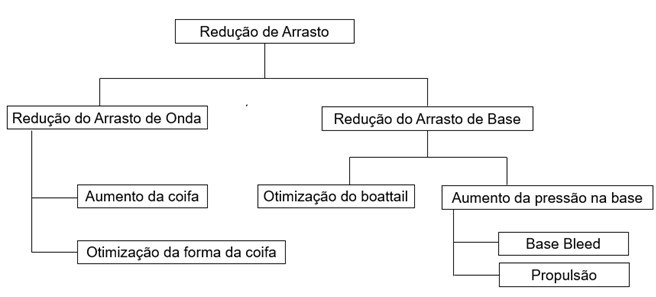
\includegraphics[width=1.0\textwidth]{foto01-reducao-arrasto.png}
	\caption[Técnicas de redução de arrasto, traduzido e adaptado.]{Técnicas de redução de arrasto \cite{Dali2018a}.}
	\label{fig1:redarrasto}
\end{figure}

Para os projetis, o arrasto se divide em três grandes grupos: o arrasto de pressão (excluindo a base), o arrasto viscoso e o arrasto de base. \citeauthor{Sahu1985} argumenta que em regime transônico, o arrasto de base pode compreender 50\% da magnitude da força de resistência do ar. Como a própria Figura \ref{fig1:redarrasto} indica, pode-se modificar a forma do \textit{boattail} ou fazer uso de uma tecnologia que aumente a pressão na base do projetil. \citeauthor{Sedney1966} apresentou em seu trabalho que modificar o \textit{boattail} pode ser uma saída complexa, pois há a possibilidade de incrementar a expansão de Prandtl-Meyer, dificultando a medição do arrasto total presente.

Com esta informação, o foco deste trabalho é estudar a influência do escoamento existente na base do armamento com alcance estendido (ER), já que há muitos desafios para o desenvolvimento destes produtos. A granada a ser estudada possui calibre 155mm (vide \autoref{fig2:cad-155mm}), devido à sua larga aplicação militar. O perfil axissimétrico possui características de design similares ao estudo feito por \citeauthor{Mahmoud2009}.

\begin{figure}[!ht]
	\centering
	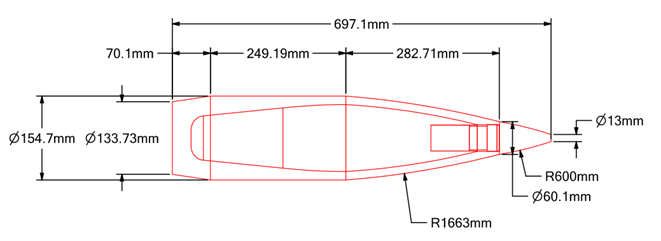
\includegraphics[width=1.0\textwidth]{foto02-cad-155mm.png}
	\caption[Granada hipotética de calibre 155mm M107 HE.]{Granada hipotética de calibre 155mm M107 HE.}
	\label{fig2:cad-155mm}
\end{figure}

Apesar de sua geometria relativamente simples, há necessidade de analisar como a injeção de massa de gases em altas temperaturas contribuem para a mudança do escoamento na base do projétil de tal forma que reduzam o arrasto ali presente. A tecnologia que aplica esses gases a partir da combustão de propelentes químicos se chama \textit{Base Bleed} (BB). A \autoref{fig3:esquemabb} apresenta como o escoamento percorre na região de maior interesse para o projeto.

\begin{figure}[!ht]
	\centering
	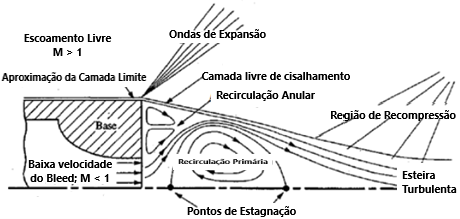
\includegraphics[width=0.8\textwidth]{foto03-esquema-bb.png}
	\caption[Escoamento supersônico na base de um projetil com \textit{Base Bleed}.]{Escoamento supersônico na base de um projetil com \textit{Base Bleed} \cite{Mathur&Dutton1996}.}
	\label{fig3:esquemabb}
\end{figure}

Para analisar qualitativamente o desempenho da tecnologia BB, o parâmetro adimensional de injeção, $Inj$, foi definido como a razão entre taxa de vazão mássica dos gases e o produto do fluxo de massa do ar livre pela área da base do projetil. Atender valores ideais deste número adimensional é um grande desafio em desenvolver um projetil com \textit{Base Bleed}. \citeauthor{Andersson1976} demonstra a importância deste controle, pois o fluxo de massa deve ser um valor muito pequeno, conforme a \autoref{fig4:andersson1976} abaixo.

\begin{figure}[!ht]
	\centering
	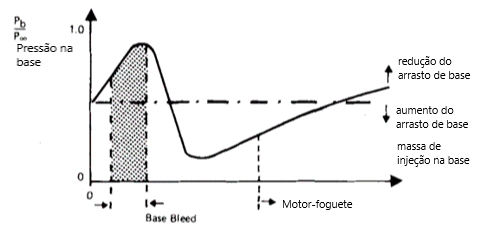
\includegraphics[width=0.8\textwidth]{foto04-grafico-andersson1976.png}
	\caption[Pressão na base por fluxo de massa.]{Pressão na base por fluxo de massa \cite{Andersson1976}.}
	\label{fig4:andersson1976}
\end{figure}

Segundo \citeauthor{Jelic2016Aug}, a existência do fenômeno de redução do arrasto de base através de um gerador de gás é datada desde a Segunda Guerra Mundial, quando se fazia uso de mísseis balísticos com traçadores que retardavam a redução de velocidade de voo, prolongando o alcance. Contudo, somente após a década de 1960 é que começou a se desenvolver pesquisas mais profundas, sendo o hidrogênio ($\textsf{H}_{2}$) o principal material usado nos geradores por ter baixo peso molecular e operar em altas temperaturas.

Os grandes questionamentos acerca deste combustível é que, apesar de muito eficiente, se permitia muito pouca estocagem dentro das munições e diminuía a vida útil delas. Outro fator relevante é que o gerador deveria conter muitos componentes, dificultando a manutenção. A solução encontrada foi trabalhar com propulsão sólida, já que se faz uso de muito menos equipamentos e o propelente poderia ser produzido através de compósitos com características adequadas às necessidades do projeto.

Segundo \citeauthor{Mahmoud2009}, para poder predizer as forças e momentos presentes na trajetória do projétil, existem quatro técnicas: os métodos empíricos; os testes em túneis de vento; simulação de fluidodinâmica computacional; e teste \textit{spark range}. As simulações recorrem métodos numéricos de fluidodinâmica computacional (CFD). Em razão das altas velocidades de disparo e das condições ambientais, considera-se o escoamento como compressível e turbulento, o que influencia nas equações de governo (Navier-Stokes) e de estado, assumindo que o ar do meio externo seja tratado como um gás perfeito. Em se tratando de turbulência, pretende-se verificar quais técnicas de abordagem sobre as equações de governo oferecem resultados satisfatórios a menor custo computacional. Em primeira análise, o objetivo é predizer os coeficientes aerodinâmicos sem a influência do \textit{Base Bleed} sob o ângulo de ataque (AOA) igual a zero.

Ao final deste trabalho é esperado concluir se a injeção de propelentes em combustão na base do projetil é um método eficiente para redução de arrasto. Para tal conclusão, será necessário validar os resultados das simulações CFD com o modelo de trajetória, como apresentado por \citeauthor{Rosendo2020}, atestando a influência da vazão e da temperatura dos gases injetados a montante do projetil. Em razão do projetil ser perfeitamente axissimétrico, a predição de trajetória é feita a partir do modelo ponto-massa modificado (MPMTM), desenvolvido por \citeauthor{Lieske1966} e padronizado pela OTAN através de um acordo de padronização chamado STANAG 4355 \cite{stanag4355}. 

Para assegurar a eficácia do software desenvolvido, uma comparação com o PRODAS®, software comercial para cálculos de dinâmica de voo para mísseis e foguetes, foi realizada considerando vários ângulos de elevação (QE) do tiro. Após a ratificação do código foram implementado os resultados do CFD para coeficiente de arrasto, seja a munição com ou sem \textit{Base Bleed}. 

\section{Revisão Bibliográfica}

O estudo sobre projéteis com alcance estendido (ER) que utilizam \textit{Base Bleed} começaram por meio de estudos experimentais que pretendiam verificar formas de reduzir o arrasto de base. \citeauthor{Sedney1966} e \citeauthor{Andersson1976} revelaram em seus trabalhos os testes realizados, sejam por testes de tiro ou em túneis de vento, com o objetivo de verificar a influência das forças de translação ou de rotação, além de verificar o efeito que o movimento rotacional causava no processo de combustão.

\begin{figure}[!ht]
	\centering
    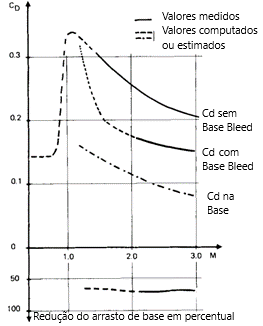
\includegraphics[width=0.6\textwidth]{foto05-grafico2-andersson1976.png}
	\caption[Coeficiente de Arrasto em função do número de Mach para um projétil calibre 120mm obtido por testes de tiro, com ou sem \textit{Base Bleed}.]{Coeficiente de Arrasto em função do número de Mach para um projétil calibre 120mm obtido por testes de tiro, com ou sem \textit{Base Bleed} \cite{Andersson1976}}
	\label{fig5:andersson1976}
\end{figure}

\citeauthor{Lieske1966} explica que o modelo MPMTM é o método principal de preparação de tabelas de tiro, desde que se saiba as propriedades de massa do projetil; os coeficientes aerodinâmicos e os valores experimentais dos testes de alcance. Para aprimoramento do trabalho, o projetil 155mm M107 foi analisado, principalmente para ajustar o coeficiente da força Magnus para as simulações. A relevância deste trabalho recai até os dias atuais, tendo em vista que os países-membros da Organização do Tratado do Atlântico Norte (OTAN) fazem uso deste recurso para desenvolver projetis de longo alcance, sejam eles estabilizados por rotação ou por aletas \cite{stanag4355}.

\citeauthor{Sahu1985} apresenta uma proposta de analisar o escoamento na base do projetil a partir de simulações computacionais com métodos numéricos para resolução das equações de Navier-Stokes. As munições 155mm foram analisadas a partir do regime transônico, pois segundo os autores, o arrasto de base representa 50\% de todo o arrasto presente na dinâmica de voo. Neste trabalho, também é possível verificar a adição de massa de gás na base do projetil, o que demonstrou os efeitos do \textit{Base Bleed} de acordo com vários parâmetros de injeção. Por fim os resultados são comparados valores experimentais e recursos semi-empíricos, seja para as granadas que possuem a tecnologia inserida ou não. A relevância deste trabalho é muito grande, pois serve como modelo de referência para todos os trabalhos com CFD que estudam arrasto de base em projéteis com alcance estendido por BB.

\citeauthor{Mathur&Dutton1996} manusearam velocímetros de laser Doppler para mensurar perfis de velocidade e turbulência na região próxima à esteira depois do corpo cilíndrico em escoamento com número de Mach (M) igual a 2,5. Neste mesmo trabalho, estimaram valores ideais de injeção do fluxo de massa na base, ou seja, o ponto que oferece a maior pressão na base, onde a região primária de recirculação é mínima, assim como a esteira turbulenta. Esse adimensional também serve até hoje como referência para calcular o efeito \textit{Base Bleed} na trajetória. 

\citeauthor{Kauri1997} já lida com simulações computacionais desenvolvidas por códigos autorais em que se aplica o modelo de turbulência $\kappa-\varepsilon$ para um escoamento supersônico (M = 1,2) a uma granada 155mm com ângulo de ataque igual a 5º. Este modelo foi escolhido porque havia o interesse em evitar problemas com as regiões dos pontos de estagnação. Neste trabalho, conclui-se que a aplicação do método baseado na vorticidade (VBPL) até oferece bons resultados para a hipótese de Boussinesq, a não ser que haja muita turbulência. 

\citeauthor{Sahu1997} resolveu numericamente as equações de Navier-Stokes de forma implícita usando dois modelos de turbulência: modelo algébrico para viscosidade turbulenta (Baldwin-Lomax) e o esquema de duas equações $\kappa-\varepsilon$. O escoamento foi aplicado apenas na região da base e após o corpo do projetil a com M = 2,46 e ângulo de ataque nulo. Para verificar os resultados, dados experimentais em testes sob mesmas condições foram obtidos e usados. A conclusão que se chegou nesta pesquisa é que os melhores resultados foram apresentados com o modelo $\kappa-\varepsilon$ para a região próxima à esteira turbulenta e prediz a pressão na base com maior precisão.

\citeauthor{Lee2006Sep} examinou diferentes perfis de orifícios para um corpo de revolução em escoamento livre a M = 2,47. As seguintes considerações foram feitas para resolver as equações de Navier-Stokes com o modelo de turbulência $\kappa-\omega$: perfil axissimétrico, escoamento compressível, com a média das massas, esquema totalmente implícito de volumes finitos e esquema \textit{upwind} de $2^{a}$ ordem para discretização espacial. A motivação inicial deste trabalho partiu do interesse em entender a redução do arrasto no regime supersônico, e verificar se estava de acordo com os resultados dos experimentos encontrados \cite{Bourdon2003Feb}.

Para averiguar a qualidade da simulação em CFD, o escoamento na saída do \textit{Base Bleed} foi calculado a partir das relações isentrópicas. O perfil da munição estudado concentrou somente a região da base, como mostra a Figura 6. Adotando um software comercial, foi possível gerar uma malha computacional que garantiu as condições de contorno e melhor convergência. As regiões com maior gradiente de pressão concentraram maior quantidade de elementos. Ao todo, 50.000 elementos foram suficientes para adquirir soluções com este domínio.

\begin{figure}[!ht]
	\centering
	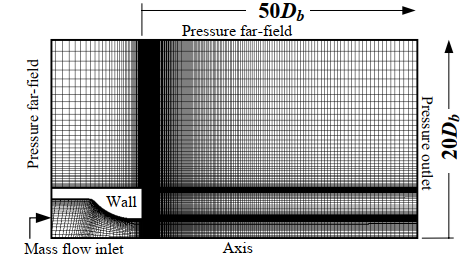
\includegraphics[width=0.6\textwidth]{foto06-malha-lee&kim.png}
	\caption[Malha computacional]{Malha computacional \cite{Lee2006Sep}}
	\label{fig6:lee2006}
\end{figure}
	
O escoamento na base pode ser visto na Figura \ref{fig7:bourdon2003} a partir dos resultados experimentais \cite{Bourdon2003Feb}. As imagens foram conseguidas utilizando a técnica de fluorescência planar em laser induzido (PLIF), que são mais profundamente detalhadas na referência. Já na \autoref{fig8:lee2006}, \citeauthor{Lee2006Sep} reproduziu computacionalmente as recirculações mais presentes próximas à base e ao eixo de simetria. Conforme I aumenta, a região primário de recirculação (PRR) é praticamente nula, embora haja a formação de uma nova recirculação próximo à camada de formação da esteira turbulenta. A conclusão confirma que há um valor adimensional que varia a cada projetil e suas condições de voo que maximiza a pressão na base. Uma configuração de design com maior área do orifício de saída dos gases ofereceu melhor controle na redução do arrasto, enquanto os casos em que a área de saída dos gases era muito pequena o incremento de injeção de massa resultou no efeito adverso na diminuição do arrasto de base. 

A influência do trabalho de \citeauthor{Lee2006Sep} é vista nas referências para as simulações em CFD sobre o arrasto de base, cujo modelo de turbulência $\kappa-\omega$ é abordado em muitos estudos devido às limitações do sistema $\kappa-\varepsilon$ em analisar a região próxima à parede. A abordagem sobre a independência de malha é percebida através dos resultados sobre o perfil de velocidades em função do raio do projetil. As condições de contorno serviram como parâmetros norteadores para aplicação na proposta da dissertação.

\begin{figure}[!ht]
	\centering
	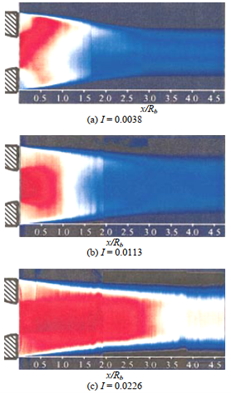
\includegraphics[width=0.5\textwidth]{foto07-bourdon2003.png}
	\caption[Visualização experimental]{Visualização experimental \cite{Bourdon2003Feb}}
	\label{fig7:bourdon2003}
\end{figure}

\begin{figure}[!ht]
	\centering
	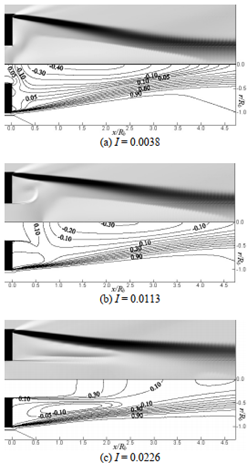
\includegraphics[width=0.5\textwidth]{foto08-base-lee&kim.png}
	\caption[Imagens computacionais baseadas no gradiente de densidade e contornos de velocidade adimensional em função do fluxo de ar no meio externo.]{Imagens computacionais baseadas no gradiente de densidade e contornos de velocidade adimensional em função do fluxo de ar no meio externo. \cite{Lee2006Sep}}
	\label{fig8:lee2006}
\end{figure}

\citeauthor{Mahmoud2009} analisou três perfis diferentes para investigar as propriedades do escoamento no entorno da munição em diferentes números de Mach com ângulo de ataque zero. Os três casos foram: com \textit{boattail}, com cavidade na base e com \textit{Base Bleed}. Além do mais, combinações entre eles foram investigadas. A maior redução de arrasto de base foi verificada quando se alinhava as três técnicas juntas. Para este caso, foi constatado uma redução de 60\% do coeficiente de arrasto em regime subsônico e algo de 20 a 30 por cento para os regimes transônico e supersônico. 
	
Ainda se tratando do trabalho de \citeauthor{Mahmoud2009}, percebe-se um detalhamento acerca dos fatores que afetam o arrasto na base do projetil, além do esclarecimento sobre o tratamento da malha em seu domínio, que pode ser visto na \autoref{fig9:mahmoud2009}. Por fim, o modelo RANS (\textit{Reynolds-Averaged Navier-Stokes}) atribuído a esta pesquisa é o Spalart-Allmaras, cujas principais aplicações envolvem pesquisas sobre aerodinâmica.  

\begin{figure}[!ht]
	\centering
	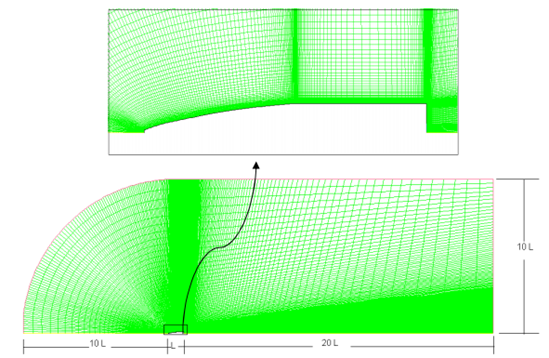
\includegraphics[width=1.0\textwidth]{foto09-malha-mahmoud2009.png}
	\caption[Modelo computacional para um projétil 155mm.]{Modelo computacional para um projétil 155mm. \cite{Mahmoud2009}}
	\label{fig9:mahmoud2009}
\end{figure}

\citeauthor{torangatti2basawaraj} concentrou as análises nas comparações entre as simulações computacionais por volumes finitos (CFD) e as abordagens semiempíricas para obtenção do arrasto, tais como MCDRAG, NSWCAP e Aero-Prediction. O modelo de turbulência RANS utilizado neste trabalho foi o $\kappa-\varepsilon$. Ao contrário da maioria dos estudos sobre CFD para problemas relacionados a este, foi usado o esquema explícito de resolução do caso. A malha computacional desenvolvida utilizando softwares comerciais apresentou uma forma de criar uma região com elementos estruturados.
	
\citeauthor{Sor2012Nov} faz um estudo similar ao anterior \cite{torangatti2basawaraj}, embora haja um aprofundamento maior acerca dos efeitos de compressibilidade e das teorias as forças aerodinâmicas. Em relação ao CFD, comparou-se os coeficientes de sustentação e de arrasto com possíveis ângulos de ataque, exceto os efeitos relacionados à rotação do projetil no disparo.

Para aprimorar o modelo com 4 graus de liberdade (4-DOF) que é desenvolvido para descrever a trajetória do projetil, estudos mais recentes foram realizados para mitigar as limitações existentes da STANAG 4355 \cite{Baranowski2013-1,Baranowski2013-2,Baranowski2013-3}. Para isso, foi necessário comparar o modelo 4-DOF com o clássico modelo de corpo rígido de 6 graus de liberdade (6-DOF) a partir de 5 ângulos de elevação para ajustar os fatores de forma, tal como descreve a STANAG 4144. O grande benefício do MPMTM é prover resultados ao menor custo computacional possível, o que significa menor tempo para resolver um problema durante uma guerra, onde este fator é crítico \cite{Baranowski2013-2}.

\citeauthor{Jelic2016Aug} teve como principal objetivo investigar vários métodos de incremento de alcance e propor soluções ótimas para estender alcance de sistemas de artilharia existentes. Dentre todas as metodologias para estender o alcance, o foco do trabalho foi pesquisar sobre \textit{Base Bleed} e motores com propulsão sólida (SRM). A pesquisa envolveu cálculos teóricos, simulações numéricas e validação através de experimentos, com resultados que confirmaram a viabilidade do conceito. 
	
\citeauthor{Xue2016Oct} desenvolveu simulações numéricas para investigar o arrasto de base e os efeitos causados pela injeção do gases pós-combustão em regime supersônico. Modelos químicos detalhados de combustão de $H_{2}-CO$ foram incorporados dentro do código computacional produzido em FORTRAN com as equações de Navier-Stokes com a aplicação do modelo RANS SST $\kappa-\omega$ \cite{Menter1994TwoequationET}. Por fim, os resultados foram validados a partir de dados experimentais e providenciaram uma melhor compreensão dos benefícios de utilizar a tecnologia \textit{Base Bleed}. O ponto alto deste estudo é permitir aplicar os efeitos da combustão dentro da pesquisa sobre a aerodinâmica do projetil. 
	
\citeauthor{belaidouni2016} estudou um armamento de calibre 122mm com perfil axissimétrico resolvendo numericamente as equações de governo para os regimes transônico e supersônico com dois modelos diferentes de turbulência por meio de volumes finitos. Ambos os resultados foram comparados com dados de predições semi-empíricas para os coeficientes aerodinâmicos. Ao contrário dos outros trabalhos, apostou-se numa malha tridimensional para o domínio do trabalho. No desenvolvimento deste projeto a injeção de massa é calculada através das equações correspondentes para a balística interna que serviram aos testes estáticos da geradora de gás. Considerando ângulo de ataque nulo, verificou-se a redução de 12\% do arrasto gerado na base da munição. A escolha final do autor pelo modelo de turbulência foi o $\kappa-\varepsilon$ realizável.
	
\citeauthor{nicolas-perez_accuracy_2017} tratou de abordar diferentes modelos RANS, DES (\textit{Detached eddy Simulation}) e LES (\textit{Large-eddy Simulation}) para estimar o coeficiente de arrasto de corpos delgados com rotação e \textit{Base Bleed} sob regimes transônico e supersônico quasi-permanentes (número de Mach entre 0,9 e 1,5). Diferentes malhas foram testadas, além de simular condições com ou sem injeção de massa gasosa na base do projetil, como na Figura \ref{fig10:nicolas2017}. Uma observação relevante neste trabalho é do esquema de fluxo ROE-FDS, pois se afirma que este recurso oferece bons resultados em casos com escoamento compressível.

\begin{figure}[!ht]
	\centering
    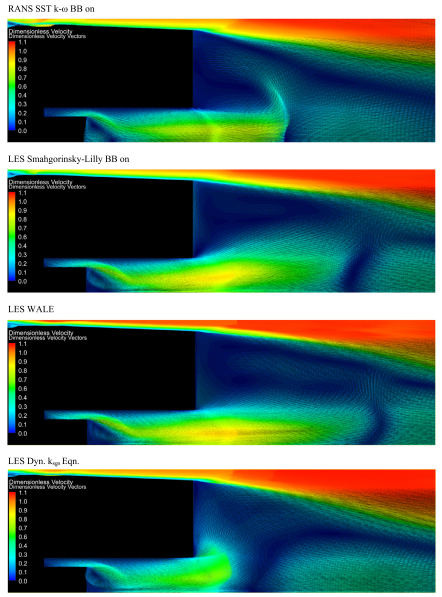
\includegraphics[width=0.5\textwidth]{chapter-01/img-cap01/foto10-nicolas2017}
	\caption[Campo de velocidade com M = 1,5 em diferentes modelos de turbulência.]{Campo de velocidade com M = 1,5 em diferentes modelos de turbulência. \cite{nicolas-perez_accuracy_2017}}
	\label{fig10:nicolas2017}
\end{figure}

A constatação sobre os resultados foi de que as abordagens RANS e DES obtiveram baixa acurácia em predizer o arrasto quando encararam o problema envolvendo uma camada de gases misturados em alta temperatura com a esteira transônica, ou seja, dificuldade em analisar a eficiência da geradora de gás. Quando inativo, os dois modelos recém citados ofereceram dados relevantes, se comparados aos valores de referência para o projeto em questão. Por fim, acrescentou o fato de que a temperatura dos gases injetados foi muito mais influente do que o peso molecular deles. Dentre os modelos de turbulência aplicados, o que melhor se adaptou aos resultados experimentais foi o caso LES WALE (\textit{Wall Adapting Local Eddy}) \cite{nicolas-perez_accuracy_2017}.

\citeauthor{Dali2018a} utilizou simulações CFD para analisar propriedades do arrasto de base em projetis com BB. Mais de um tipo de grão propelente foi usado. A meta era encontrar um caminho para efetivamente controlar o fluxo na base para reduzir o arrasto na região e otimizar utilizando um software adequado para tal. Os modelos de turbulências aplicados foram o SST $\kappa-\omega$, transição $\kappa-\kappa l-\omega$ e modelo de tensão de Reynolds (RSM). As propriedades da vazão mássica foram adimensionalizadas para melhor compreensão dos resultados. Para cada grão propelente, observou-se um parâmetro ótimo de injeção e depende da temperatura dos produtos da combustão. Em valores concretos, o arrasto reduziu em torno de 7\% para o \textit{Base Bleed} a 300K e mais de 28\% para os gases ejetados a 2500K. Este estudo também reafirmou a irrelevância do peso molecular dos produtos da combustão na redução do arrasto.
	
\citeauthor{Dali2018b}, por meio de um software proprietário CFD, analisou as duas principais formas de redução de arrasto na base de uma munição 122mm. Primeiro, a área de concentração esteve na otimização da estrutura do \textit{boattail}. Em seguida, pesquisou a influência de alterar a pressão na base do projetil com \textit{Base Bleed}, inclusive com variações de ângulos de saída dos gases em relação ao eixo longitudinal da granada. Comparando os valores obtidos com as referências encontradas em predições semi-empíricas, as diferenças foram quase imperceptíveis. Acerca da verificação com dados de radares 3D, a hipótese mais viável é do nível de ruído dos sinais, que dificultam as medidas de velocidade durante o voo. O trabalho serviu como uma referência introdutória ao assunto discutido na proposta da dissertação e oferece outras possibilidades de estudo sobre a otimização da aerodinâmica de perfis balísticos. 
	
Há trabalhos no Brasil acerca do mesmo tema, como \cite{Lucena2020,Rosendo2020,Gil2020}, que exploraram uma abordagem semelhante a esta pesquisa, contudo enfatizando a munição 114mm desenvolvida pela EMGEPRON, uma empresa estatal ligada à Marinha do Brasil. Na questão da simulação de fluidodinâmica computacional, o foco foi num domínio bidimensional e axissimétrico, com a malha não estruturada, além de não aplicar nenhum modelo de turbulência para resolver o escoamento. O OpenFOAM®, um software \textit{open-source}, foi escolhido para resolver o caso, onde se desenvolveu um modelo viável para predizer uma específica formulação para um propelente a ser utilizado em munições com alcance estendido, tendo em vista que não havia no mercado softwares comerciais para entregar tal serviço. 

O único caminho que a Marinha do Brasil até então encontrava era a partir de lançamentos balísticos de granadas como teste, o que era caro e com alto risco de segurança. Logo, através de um domínio bidimensional e axissimétrico, as equações de governo para um escoamento supersônico de uma granada calibre 114mm foram resolvidas. A conclusão desta pesquisa é que a velocidade e a temperatura de injeção dos gases do \textit{Base Bleed} possuem um valor ideal para reduzir o arrasto.

\citeauthor{Reddy2021} apresentou simulações numéricas sobre projetis calibre 155mm, seja com ou sem \textit{Base Bleed}, em regime supersônico (M = 2,26). Para tal trabalho, todo o desenvolvimento foi realizado de uma ferramenta comercial. O algoritmo aplica o modelo de turbulência SST $\kappa-\omega$, variando o ângulo de ataque entre 0 e 10 graus. Usando os recursos experimentais, as simulações foram comparadas e observou-se uma redução do coeficiente de arrasto na ordem de 14\% ao considerar o efeito \textit{Base Bleed}. 

\section{Motivação}

A dinâmica dos fluidos computacional trata-se de uma área da engenharia que vem crescendo ao longo dos últimos anos, com o avanço tecnológico. Existem inúmeros casos na natureza e na engenharia de escoamentos turbulentos com separação de fluxo que merecem ser estudados, que podem ser aprofundados e facilitados através de simulações numéricas computacionais. Nos problemas aerobalísticos, a redução de arrasto é objeto de estudo de muitas pesquisas, pois cria oportunidades em atuar na fronteira do conhecimento sobre desempenho de corpos balísticos, sejam projéteis, mísseis ou foguetes. A utilização da tecnologia \textit{Base Bleed} se apresenta como um desses casos porque permite a fabricação de equipamentos com um princípio de funcionamento relativamente simples, contudo há um desafio em matéria de design do produto e da dinâmica de fluidos existente na base do armamento.

Ao longo das últimas décadas os estudos sobre redução de arrasto na base manejando simulações numéricas computacionais tornaram-se mais frequentes. Primeiramente a abordagem CFD permitiu diminuição de testes experimentais para validação dos produtos, tendo em vista que os testes de tiro são dispendiosos, ainda mais quando se adota diferentes configurações de granadas para o disparo (com ou sem BB; com ou sem \textit{boattail}, fora os diferentes formatos). Após esses fatos, este projeto pretende aumentar a cadeia de pesquisas relacionadas com este tema no Brasil, além dos já estabelecidos \cite{Lucena2020, Rosendo2020, Gil2020}. Inclui-se ao fato de que no mercado não há modelos ou mesmo serviços que permitam estudar os efeitos da combustão do \textit{Base Bleed} de acordo com a composição química de seus propelentes. 
	
Os fenômenos de turbulência presentes no escoamento no entorno do projetil, sobretudo à jusante de sua base, serão estudados e analisados com duas abordagens RANS para descrever a turbulência do ar, principal fluido de escoamento da granada. Ao escolher os modelos RANS, espera-se obter resultados com maior agilidade e razoável confiabilidade, motivo que é amplamente mais usado na indústria ao ser comparado com modelos DES, LES ou DNS. Todavia, há de se olhar para os valores de referência ou de dados experimentais, se houver. Incorpora-se os resultados obtidos com os códigos desenvolvidos para a predição de trajetória para ofertar uma solução mais acessível se comparado ao PRODAS®, principal referência do setor aeroespacial para resolução deste tipo de problema.

Sendo assim, o presente trabalho contribuirá para a comunidade da dinâmica dos fluidos computacional tanto em relação ao estudo de metodologias para redução de arrasto na base em perfis aerodinâmicos quanto para o estudo da formulação da geradora de gás e os possíveis propelentes a serem utilizados. Há também uma contribuição para o estudo de dinâmica de corpos rígidos para oferecer soluções mais fidedignas e práticas para aplicações das normas técnicas que envolvem as tecnologias militares, como ocorrem ao fazer uso dos acordos de padronização (STANAG) para produção de armamentos com respostas mais ágeis em situações reais de combate. Com o avanço da tecnologia computacional, a mitigação dos riscos associados aos materiais aplicados à produção do BB está cada vez maior. 

\section{Objetivo de Estudo}

O presente trabalho tem como objetivo o estudo sobre a aerodinâmica de um projetil de calibre 155mm, principalmente sobre a influência da força de arrasto durante a trajetória balística. Nesta granada, será verificado o comportamento do arrasto total e na região da base, comparando os casos inerte (sem \textit{Base Bleed}) e o ativo (com \textit{Base Bleed}). Alguns parâmetros serão modificados para descobrir a melhor configuração possível do sistema BB, ou seja, qual situação que permite a maior redução do arrasto e como isso influencia a trajetória.
	
Em se tratando da fluidodinâmica computacional, as equações de governo consideram as seguintes propriedades: compressível, pois o regime de velocidades ($0,4 \leq M \leq 3,0$) apresenta variações na densidade do fluido do meio externo; permanente, logo as propriedades do fluido não variam em função do tempo; axissimétrico, porque o projetil possui um formato perfeitamente simétrico ao longo de um único eixo, o que é vantajoso para a análise CFD, pois essa aproximação é considerada uma técnica poderosa para reduzir o custo computacional \cite{Lucena2020}. Enquanto isso, as equações de estado consideraram o ar como gás ideal, assim como o gás ejetado pelo \textit{Base Bleed} e, especialmente a viscosidade dinâmica do fluido, que aplicou a Lei de Sutherland como técnica para registrar as variações do fluido de acordo com o gradiente de temperatura.

Acerca dos modelos de turbulência, o presente trabalho utilizou duas abordagens RANS. O escoamento turbulento é caracterizado por ter um comportamento difusivo, tridimensional e transiente \cite{Rezende2009}. A turbulência pode sofrer flutuações nas quais é possível aproximar de um escoamento estacionário, desde que se considere um intervalo de tempo adequado para a análise \cite{Souza2011,SilveiraNeto2002}. Em geral, a turbulência envolve grandes escalas temporais e espaciais, o que exige alto esforço computacional para obter resultados com qualidade através de simulações DNS. Por essa razão, os modelos RANS são considerados as opções mais práticas para predição numérica e são as mais empregadas pela indústria.
	
Dentre os modelos RANS existentes, foram escolhidos o Spalart-Allmaras \cite{Spalart1992} e o SST $\kappa-\omega$ (\textit{Shear-Stress Transport} $\kappa-\omega$) \cite{Menter1994TwoequationET,Menter2009}. Cada modelo possui vantagens e desvantagens a serem exploradas, principalmente em problemas aerodinâmicos. A modelagem que oferecer os resultados mais confiáveis terão seus valores acoplados ao simulador desenvolvido neste projeto, assim como os coeficientes extraídos do PRODAS® para predizer o voo da granada.

Para determinar a influência na dinâmica de voo do projetil, um código computacional foi desenvolvido em MATLAB® a partir de um trabalho de Iniciação à Pesquisa feito no Instituto Militar de Engenharia (IME) \cite{Thallyo-ENCIT2022,Thallyo2022} para comparar com o PRODAS®, fazendo uso das mesmas condições de entrada necessárias para calcular o trajeto com 4 graus de liberdade. Atingindo os objetivos, atesta-se que o software autoral está dentro do que é estabelecido pela STANAG 4355. Entretanto, a validação inicial não considera o uso da tecnologia BB, portanto é de suma importância verificar a influência da injeção de gases na base do projetil em função do alcance e do apogeu da munição. 

\section{Organização do Trabalho}

O segundo capítulo descreve uma revisão bibliográfica sobre o fenômeno físico da compressibilidade e das equações de governo que regem o fluido. A seguir, o Capítulo \ref{cap:metodos-numericos} introduz os métodos numéricos e as possíveis abordagens de discretização para as equações de transporte, com ênfase no Método de Volumes Finitos (MVF). No Capítulo \ref{cap:turbulencia}, a turbulência é apresentada como tópico de grande interesse devido aos altos números de Reynolds presentes no escoamento em torno da munição 155mm. Em especial, será tratado com mais afinco os modelos de turbulência baseados nas médias de Reynolds (RANS) e as condições necessárias para o fechamento do sistema de equações de transporte resultante. Com estes tópicos, é possível analisar e compreender os efeitos aerodinâmicos a partir das simulações CFD.

Os modelos RANS selecionados para analisar o escoamento, são Spalart-Allmaras \cite{Spalart1992} e SST $\kappa$-$\omega$ \cite{Menter1994TwoequationET,Menter2003,Menter2009}. Para a análise de trajetória, bem como a teoria necessária para implementação do modelo ponto-material modificado \cite{stanag4355}, foi desenvolvido o Capítulo \ref{cap:trajetoria}. A descrição do estudo proposto, explicando detalhadamente as condições de contorno para as simulações CFD e os valores iniciais para a predição de voo da munição 155mm, pode ser encontrada no Capítulo \ref{cap:estudo-proposto}.

O Capítulo \ref{cap:resultados} finalmente apresenta e analisa os resultados obtidos com a variação de 3 parâmetros: o diâmetro de saída, a vazão mássica e a temperatura do propelente expelido pelo sistema \textit{Base Bleed}, referente ao escoamento compressível a jusante do projetil. Os principais resultados contidos neste capítulo são os coeficientes de arrasto sem ângulo de ataque em função do número de Mach; os contornos de pressão e velocidade, além das linhas de corrente para demonstrar a formação da recirculação anular e do deslocamento da região de recirculação primária dentro da esteira turbulenta. A conclusão do trabalho encontra-se no Capítulo \ref{cap:conclusoes}, resumindo os pontos principais, e discutindo os principais problemas encontrados e recomendações para trabalhos futuros.
\chapter{Revisão Teórica}
\graphicspath{{chapter-02/img-cap02/}}

\noindent
\section{Escoamentos Compressíveis}

Para entender o conceito de compressibilidade, \citeauthor{anderson_modern_2002} afirma que escoamento compressível é definido rotineiramente como regime de densidade variável. Essa propriedade restringe-se aos fluidos. A variação infinitesimal de densidade ($d\rho$) pode ser vista na equação \ref{eq:densityeq}. 

\begin{equation} \label{eq:densityeq}
    d\rho = \rho\beta dp
\end{equation}

Sob regime de altas velocidades, o gradiente de pressão ($dp$) costuma ser elevado, donde se conclui que a variação da densidade é elevada, portanto não pode ser desprezada. Como os gases possuem alta compressibilidade ($\beta$), os valores moderados a altos de variação da pressão resultam em consideráveis mudanças de densidade, tanto que esses fluidos são comumente tratados como compressíveis.

Os fundamentos dos escoamentos compressíveis são vastos para a engenharia, muito aplicados em problemas de aerodinâmica e propulsão, como é o caso do presente trabalho. Para entender os regimes de voo nos quais o projetil é submetido, deve-se considerar os três principais campos de velocidades do fluxo de ar externo: subsônico, transônico e supersônico. Todos eles dependem da propriedade termodinâmica do gás conhecida como velocidade do som ao escoamento livre ($a_{\infty}$), cuja relação com a velocidade do escoamento livre ($U_{\infty}$) é chamada de Número de Mach ($M$), como visto na equação \ref{eq:macheq}

\begin{equation} \label{eq:macheq}
    M = \frac{U_\infty}{a_\infty}
\end{equation}

Para os casos em que o $M < 1,0$ para todo o escoamento presente, define-se o regime como subsônico. As propriedades do fluido variam continuamente e adiciona ao fato de que para se ter certeza de que o fluido está completamente inserido nestas condições se $M \leq 0,8$ \cite{anderson_modern_2002}. 

O regime transônico $0,8 \leq M \leq 1,2$ é uma situação particular do caso anterior, porque há a formação de uma região supersônica em alguns locais. Isto significa que há energia suficiente para se desencadear ondas de choque ao longo da superfície que podem alterar consideravelmente as propriedades do fluido. A Figura \ref{fig:dali2018b} apresenta um súbito acréscimo no coeficiente de arrasto ($C_D$) na faixa de $0,8 \leq M \leq 1,2$ em diferentes modelagens de turbulência RANS para munição 122 mm com \textit{Base Bleed} \cite{Dali2018b}.

\begin{figure}[!ht]
	\centering
    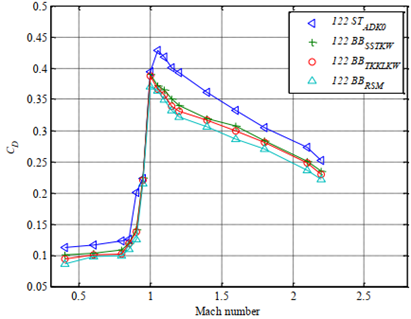
\includegraphics[width=0.5\textwidth]{foto01-dali2018b.png}
	\caption[Coeficiente de Arrasto versus Mach para o projetil com \textit{Base Bleed} pelas simulações CFD usando os modelos SST $\kappa-\omega$, Transição $\kappa-\kappa l-\kappa-\omega$ e RSM e comparando com resultados semi-empíricos \cite{Dali2018b}.]{Coeficiente de Arrasto versus Mach para o projetil com \textit{Base Bleed} pelas simulações CFD usando os modelos SST $\kappa-\omega$, Transição $\kappa-\kappa l-\kappa-\omega$ e RSM e comparando com resultados semi-empíricos \cite{Dali2018b}.}
	\label{fig:dali2018b}
\end{figure}

O regime supersônico é válido se ao longo de todo o escoamento $M \geq 1,0$. A onda de choque existente redireciona completamente o escoamento após esta região e o fluxo do fluido só se altera quando há o encontro com o corpo. No caso de gases, os escoamentos incompressíveis são casos especiais do regime subsônico e considerados apenas quando todo o fluxo se encontra em $M \leq 0,3$.

Há outras formas de classificar os escoamentos, por exemplo, a partir da viscosidade. Onde os efeitos da viscosidade, condução térmica e difusividade são relevantes podemos chamar de escoamentos viscosos. A importância deste tema é considerável, tendo em vista que afeta os modelos de turbulência utilizados para compreender o arrasto de base e as técnicas para reduzi-lo. Em todos os regimes de velocidade, o ar é analisado como um meio contínuo (hipótese do \textit{continuum}), isto é, as distâncias médias entre as moléculas do gás são infinitamente menores do que o comprimento característico do escoamento.

\section{Equações de Governo}

Neste presente trabalho, as equações de Navier-Stokes são resolvidas para um fluido compressível e em regime estacionário, logo as propriedades não variam em função do tempo. Elas servem como pré-requisito para compreender o comportamento do fluido. Em todos os casos, as formulações são obtidas a partir do equilíbrio sobre um volume de controle. Para um fluido newtoniano atuando como um gás ideal, as equações de Navier-Stokes são dadas a seguir.

\subsection{Conservação de massa}

O princípio da conservação de massa indica que, na ausência de fontes e sumidouros, a região conservará a massa a nível local. O resultado disso é explicado na equação \ref{eq:gov-continuidade} \cite{Moukalled2015, Wilcox2006}.

\begin{equation}
    \label{eq:gov-continuidade}
    \frac{\partial}{\partial x_j}(\rho u_i) = 0
\end{equation}

A equação acima considera o efeito da compressibilidade, fenômeno presente no problema a ser estudado nesta pesquisa.

\subsection{Conservação do momento linear}

O princípio da conservação do momento linear indica que, na ausência de forças externas atuando sobre um corpo, o corpo retém seu momento, ou seja, o produto da massa pelo vetor velocidade. Em suma, a conservação de momento linear só é modificada na presença de uma força líquida, causada por forças de corpo e de superfície. Na forma conservativa, a conservação do momento linear é dada pela equação \ref{eq:gov-momento} \cite{Moukalled2015, Wilcox2006}

\begin{equation}
    \label{eq:gov-momento}
    \frac{\partial}{\partial x_j}(\rho u_j u_i) = -\frac{\partial p}{\partial x_i} + \frac{\partial t_{ji}}{\partial x_j}
\end{equation}

Considerando que o fluido é newtoniano, o tensor das tensões viscosas ($t_{ji}$) é uma função linear da taxa de deformação, demonstrado pela equação \ref{eq:tau-newtoniano}:

\begin{equation}
    \label{eq:tau-newtoniano}
    t_{ij} = \mu \left(\frac{\partial u_i}{\partial x_j} + \frac{\partial u_j}{\partial x_i} \right) + \zeta\frac{\partial u_k}{\partial x_k}\delta_{ij}
\end{equation}

Onde $\mu$ é a viscosidade dinâmica e $\zeta$ é o coeficiente de dilatação da viscosidade para um gás monoatômico ($\zeta = -(2/3)\mu)$ e $\delta_{ij}$ é o delta de Kronecker. 

\subsection{Conservação de energia}

A conservação de energia é sustentada pela primeira lei da Termodinâmica, donde se conclui que a energia não é criada, tampouco destruída durante um processo; apenas se converte de forma (ex: energia química se transformando em energia cinética). Considerando um sistema isolado, a energia existente no processo é constante. Assumindo que o fluido é um gás ideal, a conservação de energia para escoamento compressível é definida pela equação \ref{eq:gov-energia} \cite{Moukalled2015, Wilcox2006}.

\begin{equation}
    \label{eq:gov-energia}
   \frac{\partial}{\partial x_j}\left[\rho u_j\left(h + \frac{1}{2}u_i u_i \right)\right] = \frac{\partial}{\partial x_j}\left(u_i t_{ij}\right) - \frac{\partial q_j}{\partial x_j}
\end{equation}

Para facilitar o cálculo da equação de energia, é necessário definir uma equação de estado \cite{Wilcox2006}. Assumindo o fluido de trabalho como um gás ideal, a lei dos gases perfeitos pode ser aplicada para correlacionar pressão, densidade e temperatura através da equação \ref{eq:densidade-ideal}

\begin{equation}
    \label{eq:densidade-ideal}
    \rho = \frac{p}{RT}
\end{equation}
%
cujo $R$, presente na equação \ref{eq:densidade-ideal}, é a constante específica do gás. O termo $e$ presente na equação \ref{eq:gov-energia} é a energia interna específica e $h = e + p/\rho$ é a entalpia específica. O vetor de fluxo de calor é definido pela Lei de Fourier, então a equação \ref{eq:lei-fourier} fica

\begin{equation}
	\label{eq:lei-fourier}
	q_j = -c_{T}\frac{\partial T}{\partial x_j}
\end{equation}
%
sendo $c_{T}$ a condutividade térmica do fluido; por aplicar a lei dos gases perfeitos, tanto a energia interna específica $e$ e a entalpia específica $h$ são definidas por

\begin{equation}
	\label{eq:equacoes-entalpia-energiainterna-calores-especificos}
	e = c_{v}T \hspace{0.5cm} \text{e} \hspace{0.5cm} h = c_{p}T
\end{equation}
%
onde $c_v$ e $c_p$ são os calores específicos para volume e pressão constantes, respectivamente. Consequentemente, a lei de Fourier \ref{eq:lei-fourier} pode ser reescrita por
%
\begin{equation}
	\label{eq:lei-fourier-NOVA}
	q_j = -c_T\frac{\partial T}{\partial x_j} = -\frac{\mu}{Pr_L}\frac{\partial h}{\partial x_j}
\end{equation}
%
o termo $Pr_L$ é o número de Prandtl laminar, definido por

\begin{equation}
	Pr_L = \frac{c_{p}\mu}{c_T}
\end{equation}
\chapter{Métodos Numéricos}\label{cap:metodos-numericos}
\graphicspath{{chapter-03/img-cap03/}}

Em todo caso de aplicação de um método numérico, deve-se iniciar pela modelagem matemática do problema. Desta forma, compreende-se como se encontra uma possível solução a partir das considerações necessárias para o problema. Após modelar o problema, faz-se necessário o uso de técnicas de discretização espaciais e temporais para transformar as equações diferenciais em equações algébricas.

As equações de Navier-Stokes podem ser escritas em variadas formas, a depender dos sistemas de coordenadas. Neste presente trabalho, as coordenadas cartesianas e ortogonais serão exploradas. Por necessidade da discretização, há alguns tipos de malhas que podem ser desenvolvidas: 

\begin{enumerate}
    \item Estruturadas: normalmente são produzidas através de uma mesma família de elementos (ex: formato quadrilátero numa malha 2D). A sua maior restrição é que normalmente se aplica estas malhas em geometria bastante simplificadas. Em malhas 3D, os erros se propagam em razão da dificuldade de controlar a distribuição de pontos;
    \item Estruturadas em blocos: há subdivisões do domínio para facilitar o refino somente onde é necessário. Contudo, há de se considerar os tratamentos nas interfaces dos subdomínios para manter a boa qualidade da malha. Em geometrias mais complexas, esta técnica costuma ter maior aplicação quando se deseja manter uma só família de elementos;
    \item Não-estruturadas: esse tipo de malha é a mais flexível para qualquer tipo de geometria. Na prática, os elementos podem ter várias formas, seja em malha 2D ou 3D. Para aplicações industriais, as malhas não-estruturadas são mais aplicadas, mesmo que haja uma perda de eficiência computacional, se comparadas com as malhas estruturadas.
\end{enumerate}

Sobre os métodos de solução, depende do problema. Seja um problema estacionário ou transiente, os problemas são altamente não-lineares, logo exige um processo iterativo para resolver. Em regra, o tipo de malha e o número de nós envolvidos é o que define a escolha pelo método mais eficiente. Por último, considera-se o critério de convergência, pois é com eles que se analisa as iterações para o método de solução escolhido. 

As mais importantes propriedades são consideradas \cite{Ferziger&Peric2020}:

\begin{enumerate}
    \item Consistência: para o método ser considerado \textit{consistente}, o valor do erro de truncamento causado pela diferença entre a equação exata e a algébrica deve ser igual a zero. Para uma simulação ter consistência, é preciso se atentar com erros na mesma ordem de precisão, principalmente termos convectivos para altos números de Reynolds ou para os termos difusivos quando se tem baixos números de Reynolds. Contudo, essa propriedade não garante que a solução das equações discretas serão as soluções exatas no limite do intervalo de tempo. Para isso ocorrer, a solução deve ser \textit{estável}.
    \item Estabilidade: uma solução numérica é \textit{estável} quando os erros não se sobressaem ao longo das iterações e garante que a solução seja limitada na mesma ordem que a solução exata. Em suma, um método estável é aquele que não diverge.
    \item Convergência: um método é dito convergente quando a solução das equações discretas tendem à solução exata da equação diferencial quando o refino de malha reduz o espaçamento dos elementos a zero. Como é difícil verificar matematicamente se a solução convergiu, testes experimentais ou valores de referências são comparados com o que se obteve numericamente. Teste de independência de malha também costumam ser feitos para verificar se a solução também é estável e consistente.
    \item Conservação: como as equações a serem resolvidas são leis de conservação, para um volume de controle uma quantidade especificada saindo deste em regime estacionário e ausente de agentes externos, é igual ao valor de entrada neste mesmo volume.
    \item Limitado: as propriedades devem satisfazer suas próprias restrições. Propriedades escalares não-negativas (ex: densidade) devem resultar em valores positivos. Sem termos-fonte, propriedades como temperatura precisam se enquadrar entre os valores das condições de contorno.
    \item Realizável: o objetivo desta propriedade é garantir que as soluções sejam realistas, principalmente quando há fenômenos complexos, como a turbulência.;
    \item Precisão: como os métodos numéricos apenas oferecem soluções aproximadas, logo possui erros que se encaixam em um desses três perfis:
    \begin{enumerate}
        \item erros de modelo: diferença entre o escoamento simulado e a solução exata do modelo matemático. No caso de escoamentos turbulentos, o modelo pode ter assumido erros durante a derivação das equações de transporte. Pode acontecer quando há uma simplificação da geometria do domínio ou da condição de contorno. Por esta razão, é muito relevante ter acesso a valores de referência, seja de testes experimentais ou de soluções diretas de turbulência, etc.
        \item erros de discretização: diferença entre a solução exata das equações de conservação e a solução algébrica do sistema de equações obtida pela discretização dessas formulações. Com refino de malha, espera-se que esses erros diminuam.  
        \item erros de iteração: diferença entre a solução exata da solução do sistema algébrico e do processo iterativo. São também chamados de \textit{erros de convergência}.
    \end{enumerate}
\end{enumerate}

Como pré-requisitos para transformar as equações analíticas em algébricas, as técnicas de discretização mais aplicadas aos problemas de dinâmicas dos fluidos computacional são descritas a seguir \cite{Ferziger&Peric2020}.

\begin{enumerate}
    \item Diferenças Finitas: é o método mais antigo e simples para resolver equações diferenciais parciais (EDP). O ponto inicial é colocar as equações de conservação na forma diferencial, sendo o domínio da solução uma malha discretizada, onde cada nó representa os valores aproximados das funções discretas obtidas através das EDP. É mais aplicado em geometrias simples, onde a malha é estruturada. A maior desvantagem é que a conservação das propriedades não é garantida, exceto se houve um tratamento específico.
    \item Volumes Finitos: neste método a malha se divide em um número finito de volumes de controle (VC) de tal forma que as propriedades do fluido são calculadas para a superfície do VC através de interpolações nos nós. Esta técnica pode ser aplicada em qualquer tipo de malha, inclusive em geometrias complexas. Esta abordagem de discretização é conservativa por natureza, sendo uma razão pela qual as análises em CFD a tornam mais usual. Sua principal desvantagem é aplicar métodos acima de segunda ordem em malhas 3D, pois exige interpolação, diferenciação e integração.
    \item Elementos Finitos: apesar de haver uma similaridade com o método de volumes finitos, suas equações são multiplicadas por funções peso antes de serem integradas num domínio. No casos mais simples, a função é aproximada por uma função linear. O resultado desta técnica é gerar um sistema de equações algébricas não-lineares. É ótimo para lidar com geometrias arbitrárias. Sua principal deficiência está na resolução de malhas não-estruturadas, pois a construção de matrizes do sistema não-linear não se permite aplicações de técnicas para solucionar.
\end{enumerate}

\section{Método dos Volumes Finitos}

Supondo que \(\phi\) seja uma variável referente a uma propriedade do fluido, o método de volumes finitos (MVF) se utiliza da forma integral da equação de transporte, como é apresentado na equação \ref{eq:volumes-finitos}.

\begin{equation}
    \label{eq:volumes-finitos}
    \int_{\forall} \frac{\partial \rho\phi}{\partial t} \hspace{0.5pt} d\forall + \int_{A} \rho\phi\boldsymbol{u}\cdot\boldsymbol{n}\hspace{0.5pt} dA = \int_{A} \Gamma_{\phi}\nabla\phi\cdot\boldsymbol{n}\hspace{0.5pt} dA + \int_{\forall} S_{\phi}\hspace{0.5pt} d\forall
\end{equation}

Os dois termos à esquerda se referem ao termo transiente por unidade de volume e o termo convectivo, respectivamente. Enquanto isso, do outro lado da equação tem-se, seguindo da esquerda para a direita, o termo difusivo e o termo-fonte. As notações em negrito são vetores. O domínio da solução é subdividido em vários volumes de controle dentro de uma malha. Acerca dos sistemas de coordenadas, este trabalho utilizará o sistema cartesiano. A abordagem de volumes finitos aplicará os resultados das integrações das equações de conservação para o centro dos volumes de controle, embora haja outras variantes. O somatório dos resultados será o valor global das equações e é por isso que o MVF se apresenta como uma técnica vantajosa para simulações CFD.

A discretização geral das equações de conservação \ref{eq:volumes-finitos} se resume a equação \ref{eq:volumes-finitos-discreta}:

\begin{equation}
    \label{eq:volumes-finitos-discreta}
    \frac{\partial \rho\phi}{\partial t}\forall + \sum_{f}^{N_{faces}}\rho_{f}\phi_{f}\boldsymbol{u}_f\boldsymbol{A}_{f} = \sum_{f}^{N_{faces}}\Gamma_{\phi}\nabla\phi_{f}\boldsymbol{A}_{f} + S_{\phi}\forall
\end{equation}
%
onde \(N_{faces}\) é igual ao número de faces envolvendo a célula; \(\phi_f\), o valor de \(\phi\) convectada através da face f; \(\rho_f\boldsymbol{u}_f\textbf{A}_f\) é o fluxo de massa através da face; \(\textbf{A}_f\), o vetor da área da face; \(\nabla\phi_f\) equivale ao gradiente de \(\phi\) na face f e \(\forall\) é o volume de controle arbitrário. A forma linearizada da equação \ref{eq:volumes-finitos-discreta} é apresentada em \ref{eq:forma-linear-mvf}:

\begin{equation}
    \label{eq:forma-linear-mvf}
    a_{p}\phi = \sum_{nb}a_{nb}\phi_{nb} + b
\end{equation}
%
onde o subscrito \(nb\) se refere às células vizinhas, enquanto que \(a_{p}\) e \(a_{nb}\) são coeficientes linearizados de \(\phi\) e \(\phi_{nb}\). O número de vizinhos depende da topologia da malha, mas o resultado é um sistema de equações com matriz de coeficientes esparsos.

\subsection{Algoritmos de resolução de escoamentos}

Há dois tipos principais de algoritmos para resolver as equações de transporte de continuidade, movimento linear e energia:

\begin{enumerate}
    \item \textit{Pressure-based}: costumam atender os casos de baixas velocidades e em regime incompressível.
    \item \textit{Density-based}: costumam ser usados em escoamentos compressíveis a altas velocidades.
\end{enumerate}

% Em ambos os casos, o campo de velocidade é obtido pela equação de movimento linear. No algoritmo , enquanto que no algoritmo \textit{density-based} resolve a densidade pela conservação de massa e o campo de pressão a partir de uma equação de estado. Por outro lado, na abordagem \textit{pressure-based}, o campo de pressão é resolvido por uma equação para a pressão ou o ajuste desta propriedade que é obtida pela manipulação das equações de continuidade e movimento linear.

Apesar de suas aplicações usuais, os métodos já foram reformulados para atender uma variedade de condições além do que foram propostos a fazer. Seja qual for o algoritmo, serão resolvidas as equações de transporte para a continuidade e movimento linear, assim como para a energia, turbulência e espécies químicas, se houver necessidade. A maneira que as equações de governo são linearizadas podem resultar numa forma “implícita” ou “explícita”. Tal explicação é demonstrada a seguir:

\begin{enumerate}
    \item Implícita: para uma dada variável, o valor a descobrir em cada volume de controle \(\forall\) é computado usando uma relação que inclui os valores existentes e desconhecidos das células vizinhas. Portanto, cada valor desejado aparecerá em mais de uma equação algébrica, onde essas equações devem ser resolvidas simultaneamente para obter o valores desconhecidos.
    \item Explícita: para uma dada variável, o valor a descobrir em cada volume de controle \(\forall\) é computado usando uma relação que inclui só os valores existentes das células vizinhas. Portanto, cada valor desejado aparecerá em apenas uma equação algébrica, onde essas equações são resolvidas sequencialmente para obter o valores desconhecidos. 
\end{enumerate}

\subsubsection{Algoritmo \textit{Pressure-Based}}

O campo de velocidade é calculado após resolver uma equação para o campo de pressão (ou o ajuste da pressão). Essa equação é derivada das conservações de massa e movimento linear, onde o campo de velocidade também satisfaz a continuidade \cite{Chorin68}. Por ser um sistema altamente não-linear e acoplado, necessita-se de um processo iterativo até atingir a convergência da solução. Há duas possibilidades de algoritmos \textit{pressure-based}, como mostra a Figura \ref{flux:pressure-based}. 

\begin{figure}[!ht]
\centering
\tikzset{every picture/.style={line width=0.75pt}} %set default line width to 0.75pt        

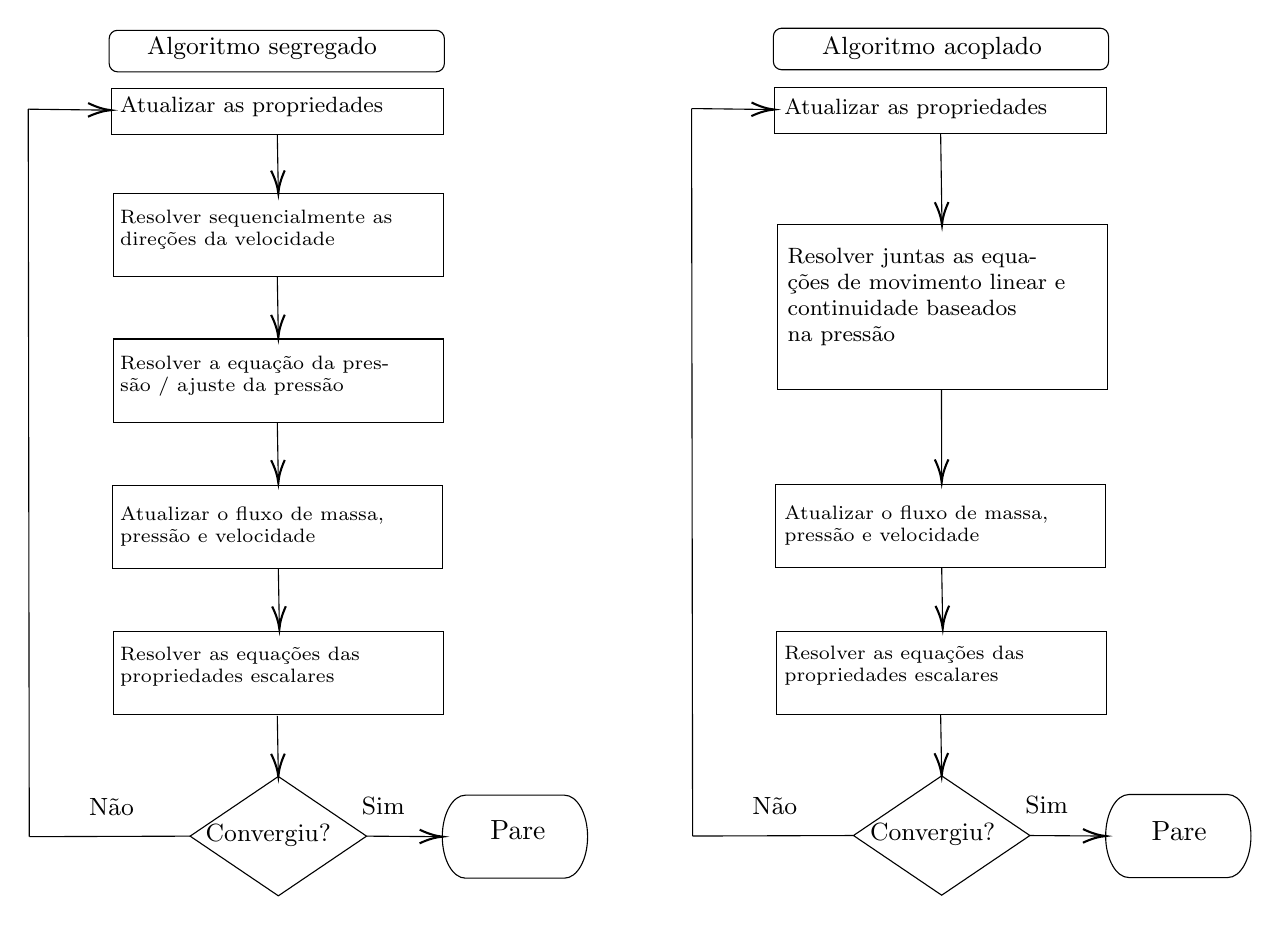
\begin{tikzpicture}[x=0.75pt,y=0.75pt,yscale=-1,xscale=1]
%uncomment if require: \path (0,476); %set diagram left start at 0, and has height of 476

%Shape: Rectangle [id:dp5456242229572967] 
\draw   (80,54.75) -- (240,54.75) -- (240,76.75) -- (80,76.75) -- cycle ;
%Shape: Rectangle [id:dp5146003696778889] 
\draw   (81,105.5) -- (240,105.5) -- (240,145.5) -- (81,145.5) -- cycle ;
%Straight Lines [id:da7993405819141195] 
\draw    (160,77) -- (160.46,103.25) ;
\draw [shift={(160.5,105.25)}, rotate = 268.99] [color={rgb, 255:red, 0; green, 0; blue, 0 }  ][line width=0.75]    (10.93,-3.29) .. controls (6.95,-1.4) and (3.31,-0.3) .. (0,0) .. controls (3.31,0.3) and (6.95,1.4) .. (10.93,3.29)   ;
%Straight Lines [id:da06909790258431547] 
\draw    (160,145.5) -- (160.47,172.75) ;
\draw [shift={(160.5,174.75)}, rotate = 269.02] [color={rgb, 255:red, 0; green, 0; blue, 0 }  ][line width=0.75]    (10.93,-3.29) .. controls (6.95,-1.4) and (3.31,-0.3) .. (0,0) .. controls (3.31,0.3) and (6.95,1.4) .. (10.93,3.29)   ;
%Shape: Rectangle [id:dp5311740933172808] 
\draw   (81,175.5) -- (240,175.5) -- (240,215.5) -- (81,215.5) -- cycle ;
%Straight Lines [id:da5901369105046621] 
\draw    (160,215.5) -- (160.47,242.75) ;
\draw [shift={(160.5,244.75)}, rotate = 269.02] [color={rgb, 255:red, 0; green, 0; blue, 0 }  ][line width=0.75]    (10.93,-3.29) .. controls (6.95,-1.4) and (3.31,-0.3) .. (0,0) .. controls (3.31,0.3) and (6.95,1.4) .. (10.93,3.29)   ;
%Shape: Rectangle [id:dp4189524190256626] 
\draw   (80.5,246) -- (239.5,246) -- (239.5,286) -- (80.5,286) -- cycle ;
%Straight Lines [id:da7692950512064372] 
\draw    (160.5,286) -- (160.97,313.25) ;
\draw [shift={(161,315.25)}, rotate = 269.02] [color={rgb, 255:red, 0; green, 0; blue, 0 }  ][line width=0.75]    (10.93,-3.29) .. controls (6.95,-1.4) and (3.31,-0.3) .. (0,0) .. controls (3.31,0.3) and (6.95,1.4) .. (10.93,3.29)   ;
%Shape: Rectangle [id:dp5046834721515459] 
\draw   (81,316.5) -- (240,316.5) -- (240,356.5) -- (81,356.5) -- cycle ;
%Flowchart: Decision [id:dp6914527803231723] 
\draw   (160.5,386.25) -- (203,415) -- (160.5,443.75) -- (118,415) -- cycle ;
%Straight Lines [id:da641257311737564] 
\draw    (160,357) -- (160.47,384.25) ;
\draw [shift={(160.5,386.25)}, rotate = 269.02] [color={rgb, 255:red, 0; green, 0; blue, 0 }  ][line width=0.75]    (10.93,-3.29) .. controls (6.95,-1.4) and (3.31,-0.3) .. (0,0) .. controls (3.31,0.3) and (6.95,1.4) .. (10.93,3.29)   ;
%Straight Lines [id:da970365971837885] 
\draw    (203,415) -- (237.5,415.24) ;
\draw [shift={(239.5,415.25)}, rotate = 180.39] [color={rgb, 255:red, 0; green, 0; blue, 0 }  ][line width=0.75]    (10.93,-3.29) .. controls (6.95,-1.4) and (3.31,-0.3) .. (0,0) .. controls (3.31,0.3) and (6.95,1.4) .. (10.93,3.29)   ;
%Flowchart: Terminator [id:dp947666633166445] 
\draw   (250.7,395.25) -- (298.3,395.25) .. controls (304.49,395.25) and (309.5,404.2) .. (309.5,415.25) .. controls (309.5,426.3) and (304.49,435.25) .. (298.3,435.25) -- (250.7,435.25) .. controls (244.51,435.25) and (239.5,426.3) .. (239.5,415.25) .. controls (239.5,404.2) and (244.51,395.25) .. (250.7,395.25) -- cycle ;
%Straight Lines [id:da7859174596491716] 
\draw    (40,64.75) -- (40.5,415.25) ;
%Straight Lines [id:da7515603235516235] 
\draw    (118,415) -- (40.5,415.25) ;
%Straight Lines [id:da6386965161765668] 
\draw    (40,64.75) -- (77.77,65.21) ;
\draw [shift={(79.77,65.23)}, rotate = 180.69] [color={rgb, 255:red, 0; green, 0; blue, 0 }  ][line width=0.75]    (10.93,-3.29) .. controls (6.95,-1.4) and (3.31,-0.3) .. (0,0) .. controls (3.31,0.3) and (6.95,1.4) .. (10.93,3.29)   ;
%Shape: Rectangle [id:dp6955840613043904] 
\draw   (399.6,54.45) -- (559.6,54.45) -- (559.6,76.45) -- (399.6,76.45) -- cycle ;
%Shape: Rectangle [id:dp2470197636955902] 
\draw   (401.1,120.5) -- (560.1,120.5) -- (560.1,200) -- (401.1,200) -- cycle ;
%Straight Lines [id:da36804399782889763] 
\draw    (479.6,76.7) -- (480.22,118.5) ;
\draw [shift={(480.25,120.5)}, rotate = 269.15] [color={rgb, 255:red, 0; green, 0; blue, 0 }  ][line width=0.75]    (10.93,-3.29) .. controls (6.95,-1.4) and (3.31,-0.3) .. (0,0) .. controls (3.31,0.3) and (6.95,1.4) .. (10.93,3.29)   ;
%Straight Lines [id:da9013024578546147] 
\draw    (480,199.75) -- (480.1,242.45) ;
\draw [shift={(480.1,244.45)}, rotate = 269.87] [color={rgb, 255:red, 0; green, 0; blue, 0 }  ][line width=0.75]    (10.93,-3.29) .. controls (6.95,-1.4) and (3.31,-0.3) .. (0,0) .. controls (3.31,0.3) and (6.95,1.4) .. (10.93,3.29)   ;
%Shape: Rectangle [id:dp4764395574363469] 
\draw   (400.1,245.7) -- (559.1,245.7) -- (559.1,285.7) -- (400.1,285.7) -- cycle ;
%Straight Lines [id:da1290244750194034] 
\draw    (480.1,285.7) -- (480.57,312.95) ;
\draw [shift={(480.6,314.95)}, rotate = 269.02] [color={rgb, 255:red, 0; green, 0; blue, 0 }  ][line width=0.75]    (10.93,-3.29) .. controls (6.95,-1.4) and (3.31,-0.3) .. (0,0) .. controls (3.31,0.3) and (6.95,1.4) .. (10.93,3.29)   ;
%Shape: Rectangle [id:dp6352478239859609] 
\draw   (400.6,316.2) -- (559.6,316.2) -- (559.6,356.2) -- (400.6,356.2) -- cycle ;
%Flowchart: Decision [id:dp17744394343128667] 
\draw   (480.1,385.95) -- (522.6,414.7) -- (480.1,443.45) -- (437.6,414.7) -- cycle ;
%Straight Lines [id:da885342291248687] 
\draw    (479.6,356.7) -- (480.07,383.95) ;
\draw [shift={(480.1,385.95)}, rotate = 269.02] [color={rgb, 255:red, 0; green, 0; blue, 0 }  ][line width=0.75]    (10.93,-3.29) .. controls (6.95,-1.4) and (3.31,-0.3) .. (0,0) .. controls (3.31,0.3) and (6.95,1.4) .. (10.93,3.29)   ;
%Straight Lines [id:da9995731339683702] 
\draw    (522.6,414.7) -- (557.1,414.94) ;
\draw [shift={(559.1,414.95)}, rotate = 180.39] [color={rgb, 255:red, 0; green, 0; blue, 0 }  ][line width=0.75]    (10.93,-3.29) .. controls (6.95,-1.4) and (3.31,-0.3) .. (0,0) .. controls (3.31,0.3) and (6.95,1.4) .. (10.93,3.29)   ;
%Flowchart: Terminator [id:dp03700567233492813] 
\draw   (570.3,394.95) -- (617.9,394.95) .. controls (624.09,394.95) and (629.1,403.9) .. (629.1,414.95) .. controls (629.1,426) and (624.09,434.95) .. (617.9,434.95) -- (570.3,434.95) .. controls (564.11,434.95) and (559.1,426) .. (559.1,414.95) .. controls (559.1,403.9) and (564.11,394.95) .. (570.3,394.95) -- cycle ;
%Straight Lines [id:da714897424737142] 
\draw    (359.6,64.45) -- (360.1,414.95) ;
%Straight Lines [id:da5698935015214337] 
\draw    (437.6,414.7) -- (360.1,414.95) ;
%Straight Lines [id:da037788770764761725] 
\draw    (359.6,64.45) -- (397.37,64.91) ;
\draw [shift={(399.37,64.93)}, rotate = 180.69] [color={rgb, 255:red, 0; green, 0; blue, 0 }  ][line width=0.75]    (10.93,-3.29) .. controls (6.95,-1.4) and (3.31,-0.3) .. (0,0) .. controls (3.31,0.3) and (6.95,1.4) .. (10.93,3.29)   ;
%Rounded Rect [id:dp7855365314760501] 
\draw   (79,30.75) .. controls (79,28.54) and (80.79,26.75) .. (83,26.75) -- (236.5,26.75) .. controls (238.71,26.75) and (240.5,28.54) .. (240.5,30.75) -- (240.5,42.75) .. controls (240.5,44.96) and (238.71,46.75) .. (236.5,46.75) -- (83,46.75) .. controls (80.79,46.75) and (79,44.96) .. (79,42.75) -- cycle ;
%Rounded Rect [id:dp7552054721421797] 
\draw   (399,29.75) .. controls (399,27.54) and (400.79,25.75) .. (403,25.75) -- (556.5,25.75) .. controls (558.71,25.75) and (560.5,27.54) .. (560.5,29.75) -- (560.5,41.75) .. controls (560.5,43.96) and (558.71,45.75) .. (556.5,45.75) -- (403,45.75) .. controls (400.79,45.75) and (399,43.96) .. (399,41.75) -- cycle ;

% Text Node
\draw (83,57.5) node [anchor=north west][inner sep=0.75pt]  [font=\footnotesize] [align=left] {Atualizar as propriedades};
% Text Node
\draw (83,112) node [anchor=north west][inner sep=0.75pt]  [font=\scriptsize] [align=left] {Resolver sequencialmente as\\direções da velocidade};
% Text Node
\draw (83,182.5) node [anchor=north west][inner sep=0.75pt]  [font=\scriptsize] [align=left] {Resolver a equação da pres-\\são / ajuste da pressão};
% Text Node
\draw (83,255) node [anchor=north west][inner sep=0.75pt]  [font=\scriptsize] [align=left] {Atualizar o fluxo de massa, \\pressão e velocidade};
% Text Node
\draw (83,322.5) node [anchor=north west][inner sep=0.75pt]  [font=\scriptsize] [align=left] {Resolver as equações das \\propriedades escalares};
% Text Node
\draw (124.25,408) node [anchor=north west][inner sep=0.75pt]  [font=\small] [align=left] {Convergiu?};
% Text Node
\draw (258.5,406.25) node [anchor=north west][inner sep=0.75pt]  [font=\normalsize] [align=left] {\begin{minipage}[lt]{24.27pt}\setlength\topsep{0pt}
\begin{center}
Pare
\end{center}

\end{minipage}};
% Text Node
\draw (86.75,401) node  [font=\small] [align=left] {\begin{minipage}[lt]{26.18pt}\setlength\topsep{0pt}
Não
\end{minipage}};
% Text Node
\draw (218.25,400.5) node  [font=\small] [align=left] {\begin{minipage}[lt]{26.18pt}\setlength\topsep{0pt}
Sim
\end{minipage}};
% Text Node
\draw (403,58.7) node [anchor=north west][inner sep=0.75pt]  [font=\footnotesize] [align=left] {Atualizar as propriedades};
% Text Node
\draw (403,254.7) node [anchor=north west][inner sep=0.75pt]  [font=\scriptsize] [align=left] {Atualizar o fluxo de massa,\\pressão e velocidade};
% Text Node
\draw (403,322.2) node [anchor=north west][inner sep=0.75pt]  [font=\scriptsize] [align=left] {Resolver as equações das\\propriedades escalares};
% Text Node
\draw (444.35,407.45) node [anchor=north west][inner sep=0.75pt]  [font=\small] [align=left] {Convergiu?};
% Text Node
\draw (577.1,406.7) node [anchor=north west][inner sep=0.75pt]  [font=\normalsize] [align=left] {\begin{minipage}[lt]{24.27pt}\setlength\topsep{0pt}
\begin{center}
Pare
\end{center}

\end{minipage}};
% Text Node
\draw (406.35,400.7) node  [font=\small] [align=left] {\begin{minipage}[lt]{26.18pt}\setlength\topsep{0pt}
Não
\end{minipage}};
% Text Node
\draw (537.85,400.2) node  [font=\small] [align=left] {\begin{minipage}[lt]{26.18pt}\setlength\topsep{0pt}
Sim
\end{minipage}};
% Text Node
\draw (404.6,130.25) node [anchor=north west][inner sep=0.75pt]  [font=\footnotesize] [align=left] {Resolver juntas as equa-\\ções de movimento linear e\\ continuidade baseados\\ na pressão};
% Text Node
\draw (96,28.75) node [anchor=north west][inner sep=0.75pt]  [font=\small] [align=left] {Algoritmo segregado};
% Text Node
\draw (421.25,28.75) node [anchor=north west][inner sep=0.75pt]  [font=\small] [align=left] {Algoritmo acoplado};\
\end{tikzpicture}
\caption[Fluxogramas para algoritmo \textit{pressure-based} segregado e acoplado.]{Fluxogramas para algoritmo \textit{pressure-based} segregado e acoplado \cite{fluent2021ansys}.}
\label{flux:pressure-based}
\end{figure}

Ambos os casos tem prós e contras, quando analisadas as convergências das soluções e o uso de memória computacional. A \autoref{tab:esquema-comparacao-segregado-acoplado} resume as diferenças entre os tipos de algoritmos.

\begin{table}[ht]
\centering
\vspace{0.5cm}
\caption[Comparações entre os algoritmos segregados e acoplados.]{Comparações entre os algoritmos segregados e acoplados.}
\begin{tabular}[c]{c|c|c}
Tipo de algoritmo & Convergência da solução & Uso de memória \\
\hline
Segregado & Baixo & Baixo \\
Acoplado & Baixo & Alto
\end{tabular}
\label{tab:esquema-comparacao-segregado-acoplado}
\end{table}

As comparações da \autoref{tab:esquema-comparacao-segregado-acoplado} são baseadas nos desempenhos dos próprios algoritmos.

\subsubsection{Algoritmo \textit{Density-Based}}

Esse algoritmo busca resolver as equações de transporte para a conservação da massa, movimento linear e energia simultaneamente \cite{Weiss1995PreconditioningAT, Weiss1997IMPLICITSO, Weiss1999ImplicitSO}. As equações adicionais de turbulência e espécies químicas (se houver) são resolvidas sequencialmente. Assim como o método \textit{pressure-based}, há a necessidade de se resolver iterativamente até atingir a convergência da solução. Na Figura \ref{fig:density-based} é apresentado o fluxograma para a compreensão do método \cite{fluent2021ansys}.

\begin{figure}[!ht]
    \centering

\tikzset{every picture/.style={line width=0.75pt}} %set default line width to 0.75pt        

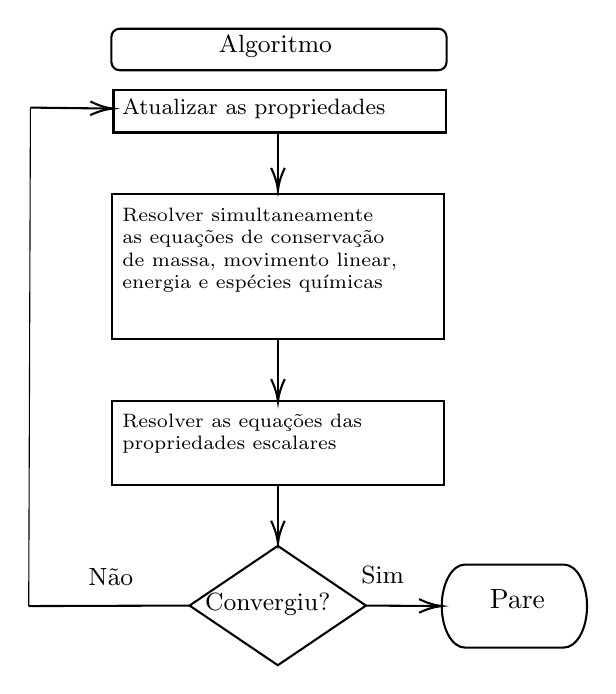
\begin{tikzpicture}[x=0.75pt,y=0.75pt,yscale=-1,xscale=1]
%uncomment if require: \path (0,476); %set diagram left start at 0, and has height of 476

%Shape: Rectangle [id:dp5456242229572967] 
\draw  [line width=0.75]  (231,60.25) -- (391,60.25) -- (391,80.75) -- (231,80.75) -- cycle ;
%Shape: Rectangle [id:dp5146003696778889] 
\draw  [line width=0.75]  (230.5,110.25) -- (390.25,110.25) -- (390.25,180.25) -- (230.5,180.25) -- cycle ;
%Shape: Rectangle [id:dp5046834721515459] 
\draw  [line width=0.75]  (230.5,210.25) -- (390.33,210.25) -- (390.33,250.5) -- (230.5,250.5) -- cycle ;
%Flowchart: Decision [id:dp6914527803231723] 
\draw  [line width=0.75]  (310.17,279.92) -- (352.67,308.67) -- (310.17,337.42) -- (267.67,308.67) -- cycle ;
%Straight Lines [id:da970365971837885] 
\draw [line width=0.75]    (352.67,308.67) -- (387.17,308.9) ;
\draw [shift={(389.17,308.92)}, rotate = 180.39] [color={rgb, 255:red, 0; green, 0; blue, 0 }  ][line width=0.75]    (10.93,-3.29) .. controls (6.95,-1.4) and (3.31,-0.3) .. (0,0) .. controls (3.31,0.3) and (6.95,1.4) .. (10.93,3.29)   ;
%Flowchart: Terminator [id:dp947666633166445] 
\draw  [line width=0.75]  (400.37,288.92) -- (447.97,288.92) .. controls (454.15,288.92) and (459.17,297.87) .. (459.17,308.92) .. controls (459.17,319.96) and (454.15,328.92) .. (447.97,328.92) -- (400.37,328.92) .. controls (394.18,328.92) and (389.17,319.96) .. (389.17,308.92) .. controls (389.17,297.87) and (394.18,288.92) .. (400.37,288.92) -- cycle ;
%Straight Lines [id:da7515603235516235] 
\draw [line width=0.75]    (267.67,308.67) -- (190.17,308.92) ;
%Straight Lines [id:da6386965161765668] 
\draw [line width=0.75]    (191,68.75) -- (228.77,69.21) ;
\draw [shift={(230.77,69.23)}, rotate = 180.69] [color={rgb, 255:red, 0; green, 0; blue, 0 }  ][line width=0.75]    (10.93,-3.29) .. controls (6.95,-1.4) and (3.31,-0.3) .. (0,0) .. controls (3.31,0.3) and (6.95,1.4) .. (10.93,3.29)   ;
%Rounded Rect [id:dp7855365314760501] 
\draw  [line width=0.75]  (230,34.75) .. controls (230,32.54) and (231.79,30.75) .. (234,30.75) -- (387.5,30.75) .. controls (389.71,30.75) and (391.5,32.54) .. (391.5,34.75) -- (391.5,46.75) .. controls (391.5,48.96) and (389.71,50.75) .. (387.5,50.75) -- (234,50.75) .. controls (231.79,50.75) and (230,48.96) .. (230,46.75) -- cycle ;
%Straight Lines [id:da9465483108271935] 
\draw    (310.25,80.75) -- (310.25,106.75) ;
\draw [shift={(310.25,108.75)}, rotate = 270] [color={rgb, 255:red, 0; green, 0; blue, 0 }  ][line width=0.75]    (10.93,-3.29) .. controls (6.95,-1.4) and (3.31,-0.3) .. (0,0) .. controls (3.31,0.3) and (6.95,1.4) .. (10.93,3.29)   ;
%Straight Lines [id:da3995043167173449] 
\draw    (310.25,180) -- (310.25,208.5) ;
\draw [shift={(310.25,210.5)}, rotate = 270] [color={rgb, 255:red, 0; green, 0; blue, 0 }  ][line width=0.75]    (10.93,-3.29) .. controls (6.95,-1.4) and (3.31,-0.3) .. (0,0) .. controls (3.31,0.3) and (6.95,1.4) .. (10.93,3.29)   ;
%Straight Lines [id:da04251926302512321] 
\draw    (310.25,250.75) -- (310.25,276.75) ;
\draw [shift={(310.25,278.75)}, rotate = 270] [color={rgb, 255:red, 0; green, 0; blue, 0 }  ][line width=0.75]    (10.93,-3.29) .. controls (6.95,-1.4) and (3.31,-0.3) .. (0,0) .. controls (3.31,0.3) and (6.95,1.4) .. (10.93,3.29)   ;
%Straight Lines [id:da9763303419571623] 
\draw    (191,68.75) -- (190.17,308.92) ;

% Text Node
\draw (234,63.5) node [anchor=north west][inner sep=0.75pt]  [font=\footnotesize] [align=left] {Atualizar as propriedades};
% Text Node
\draw (234,116) node [anchor=north west][inner sep=0.75pt]  [font=\scriptsize] [align=left] {Resolver simultaneamente\\as equações de conservação \\de massa, movimento linear,\\ energia e espécies químicas};
% Text Node
\draw (234,214.92) node [anchor=north west][inner sep=0.75pt]  [font=\scriptsize] [align=left] {Resolver as equações das\\propriedades escalares};
% Text Node
\draw (273.92,301.67) node [anchor=north west][inner sep=0.75pt]  [font=\small] [align=left] {Convergiu?};
% Text Node
\draw (408.17,299.92) node [anchor=north west][inner sep=0.75pt]  [font=\normalsize] [align=left] {\begin{minipage}[lt]{24.27pt}\setlength\topsep{0pt}
\begin{center}
Pare
\end{center}

\end{minipage}};
% Text Node
\draw (236.42,294.67) node  [font=\small] [align=left] {\begin{minipage}[lt]{26.18pt}\setlength\topsep{0pt}
Não
\end{minipage}};
% Text Node
\draw (367.92,294.17) node  [font=\small] [align=left] {\begin{minipage}[lt]{26.18pt}\setlength\topsep{0pt}
Sim
\end{minipage}};
% Text Node
\draw (280.5,32.75) node [anchor=north west][inner sep=0.75pt]  [font=\small] [align=left] {Algoritmo};

\end{tikzpicture}
\caption[Fluxograma para algoritmo \textit{density-based}]{Fluxograma para algoritmo \textit{density-based} \cite{fluent2021ansys}.}
\label{fig:density-based}
\end{figure}

\subsection{Discretização espacial}

Assumindo que se trata de um problema em regime estacionário, o termo \(\frac{\partial \rho\phi}{\partial t}\forall\) pode ser desconsiderado da equação \ref{eq:volumes-finitos}, resultando na equação \ref{eq:volumes-finitos-estacionaria}:

\begin{equation}
    \label{eq:volumes-finitos-estacionaria}
    \int_{A} \rho\phi\boldsymbol{u}\cdot\boldsymbol{n}\hspace{0.5pt} dA = \int_{A} \Gamma_{\phi}\nabla\phi\cdot\boldsymbol{n}\hspace{0.5pt} dA + \int_{\forall} S_{\phi}\hspace{0.5pt} d\forall
\end{equation}

Os valores discretos de \(\phi\) são obtidos no centros dos volumes de controle, mas os valores referentes às faces de \(\phi\) são interpolados através dos valores centrais dos volumes de controle \cite{Rezende2009}. Os seguintes esquemas de discretização espacial serão tratados: diferenças centrais; \textit{upwind} de 1\textsuperscript{a} ordem e 2\textsuperscript{a} ordem e QUICK.

\subsubsection{Esquema de diferenças centrais}

O valor da variável na face do volume de controle \(\phi_{f}\) é calculado da seguinte forma no esquema de diferenças centrais (CDS), conforme equação \ref{eq:esquema-CDS} \cite{Rezende2009}.

\begin{equation}
    \label{eq:esquema-CDS}
    \phi_f = \frac{1}{2}\left(\phi_0+\phi_1\right)+\frac{1}{2}\left(\nabla\phi_0\cdot\overrightarrow{r_0}+\nabla\phi_1\cdot\overrightarrow{r_1}\right)
\end{equation}
%
sendo 0 e 1 os índices das células representadas na Figura \ref{fig:volume-ANSYS-2021R2}, sendo \(\overrightarrow{r}\) o vetor deslocamento que liga o centro da célula a montante à face do volume de controle. A Figura \ref{fig:volume-ANSYS-2021R2} ilustra a discretização de uma célula triangular bidimensional como exemplo de volume de controle \cite{fluent2021ansys}.

\begin{figure}[!ht] 
	\centering
	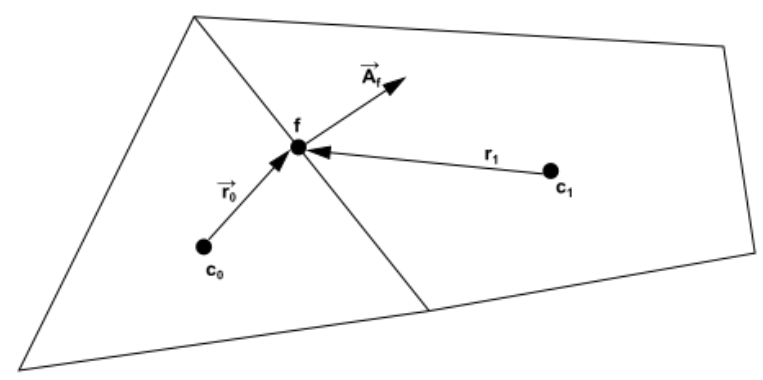
\includegraphics[width=0.5\textwidth]{foto01-volume-fluent.png}
    \caption[Volume de controle usado para ilustrar a discretização da equação do transporte escalar.]{Volume de controle usado para ilustrar a discretização da equação do transporte escalar \cite{fluent2021ansys}.}
	\label{fig:volume-ANSYS-2021R2}
\end{figure}

Portanto, esse esquema não reconhece a direção do escoamento ou a influência da convecção em relação à difusão \cite{malalasekera2007}. Ainda se tratando da mesma referência, o CDS não é um modelo mais indicado para resolver casos genéricos e, por esta razão, os esquemas \textit{upwind} de 1\textsuperscript{a} e 2\textsuperscript{a} ordem, além do QUICK serão apresentados.

\subsubsection{Esquema \textit{upwind} de primeira ordem}

Considerando que o esquema anterior tem uma dificuldade de identificar a direção do escoamento, o esquema \textit{upwind} de 1\textsuperscript{a} ordem (UDS-1) determina o valor de \(\phi_f\) convectada na face \(f\) a partir do valor \(\phi_{up}\) a montante. A equação \ref{eq:esquema-upwind-1aordem} apresenta a aproximação inicial para as propriedades de interesse do fluido \cite{Rezende2009}.

\begin{equation}\label{eq:esquema-upwind-1aordem}
	\phi_f = \phi_{up}
\end{equation}

\citeauthor{malalasekera2007} explica que a simplicidade deste método é o que fez ser tão aplicado em simulações CFD até os dias atuais. O seu maior entrave está na produção de um erro que aparenta um comportamento difusivo e por essa razão se chama de "falsa difusão". Esse fenômeno se agrava em casos que o número de Reynolds é elevado, logo não costuma ser aplicado em problemas com necessidade de alta precisão.

\subsubsection{Esquema \textit{upwind} de segunda ordem}

Quando uma precisão de segunda ordem é requerida, utiliza-se uma interpolação linear com mais de um elemento adjacente, onde a precisão de ordem elevada é atingida a partir da expansão por série de Taylor da solução no centroide do volume de controle \cite{Rezende2009}. O esquema \textit{upwind} de 2ª ordem (UDS-2) envolve dois valores a montante, resultando na seguinte equação \ref{eq:esquema-upwind-2aordem} para \(\phi_f\):

\begin{equation} \label{eq:esquema-upwind-2aordem}
    \phi_f = \phi_{c_0} + \left(\nabla\phi\cdot\overrightarrow{r}\right)_{up}
\end{equation}

Considere \(\phi_{c_0}\) o valor de \(\phi\) na célula central. A equação \ref{eq:esquema-upwind-2aordem} assume que o escoamento está na direção positiva, já que a face analisada está a leste, logo o subscrito \(e\) surge na variável \(\phi_e\) na equação~\ref{eq}. Na direção negativa, o gradiente da função ainda terá a mesma magnitude, porém com sentido inverso. Para definir o gradiente de \(\phi\), \(\nabla\phi\), assume-se neste projeto que foi usado o método dos mínimos quadrados \cite{Anderson1994}, cuja proposta é admitir que a solução varia linearmente. Conforme demonstrado na equação \ref{eq:gradiente-minimos-quadrados}, espera-se que calcule os valores para as células \(c0\) e \(ci\) (ver \autoref{fig:minimos-quadrados})

\begin{equation} \label{eq:gradiente-minimos-quadrados}
    \left(\nabla\phi\right)_{c0} \cdot \Delta r_i = \phi_{ci} - \phi_{c0}
\end{equation}

\begin{figure}[!ht]
	\centering
	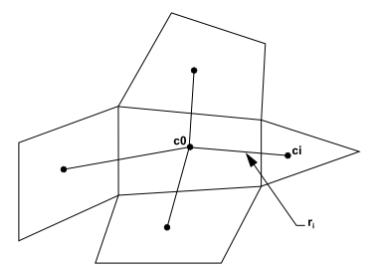
\includegraphics[width=0.5\textwidth]{foto02-minimos-quadrados.png}
	\caption[Avaliação do gradiente do volume de controle]{Avaliação do gradiente do volume de controle \cite{fluent2021ansys}.}
	\label{fig:minimos-quadrados}
\end{figure}
 
\subsubsection{Esquema QUICK}

O esquema QUICK \cite{Leonard1990} se baseia em uma média ponderada entre os esquemas \textit{upwind} de 2ª ordem (UDS-2) e diferenças centradas (CDS). Para um problema em 1-D, temos a \autoref{fig:ansys-QUICK} para explicar a lógica por trás dessa interpolação da seguinte forma (vide equação \ref{eq:esquema-quick}):

\begin{equation}
	\label{eq:esquema-quick}
	\phi_e = \theta\left[\frac{S_d}{S_c+S_d}\phi_P + \frac{S_c}{S_c+S_d}\phi_E \right] + (1 - \theta)\left[\frac{S_u+2S_c}{S_u+S_c}\phi_P - \frac{S_c}{S_c+S_u}\phi_W \right]
\end{equation}

\begin{figure}[!ht]
	\centering
	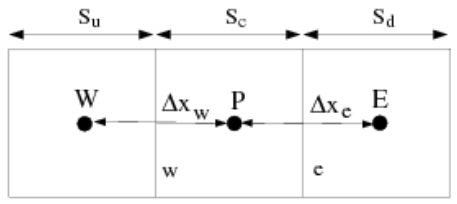
\includegraphics[width=0.5\textwidth]{foto03-quick-1d.png}  
	\caption[Esquema QUICK para um escoamento unidimensional.]{Esquema QUICK para um escoamento unidimensional \cite{fluent2021ansys}.}
	\label{fig:ansys-QUICK}
\end{figure}

A equação acima resulta no esquema CDS quando \(\theta = 1\) e no UDS-2 quando \(\theta = 0\). A versão tradicional do QUICK \cite{Leonard1979} considera \(\theta = 1/8\). Comparado aos esquemas \textit{upwind} de 1ª ordem e diferenças centrais, é um modelo mais eficiente. A falsa difusão é baixa, mas deve-se levar em consideração de desvios nos resultados quando a geometria do problema for complexa \cite{Leonard1979}.

\subsection{Relaxação dos termos de alta ordem}

A proposta da relaxação é melhorar a inicialização e o comportamento da solução geral das simulações do escoamento quando discretizações espaciais de ordem superior são utilizadas (acima de 1ª ordem) \cite{fluent2021ansys}. A sub-relaxação desses termos segue a equação \ref{eq:relaxacao-altaordem} para qualquer propriedade \(\phi\):

\begin{equation}
    \label{eq:relaxacao-altaordem}
    \phi_{novo} = \phi_{velho} + f(\phi_{novo} - \phi_{velho})
\end{equation}

Considera-se como padrão \(f = 0,25\) em regime estacionário, foco deste presente trabalho.

\subsection{Método Multigrid}

O método \textit{Multigrid} \cite{Hutchinson1986} é usado porque acelera a convergência através de uma sequência de correções em uma série de níveis de refino da malha. É um método bom para remover erros locais (alta frequência) e menos efetivo em erros globais (baixa frequência).

O \textit{Multigrid} é bastante eficiente quando se trata do esquema \textit{density-based} para remover os erros de alta frequência. Ele trabalha com uma sequência de malhas \(M_1\) até \(M_n\), cada vez mais grossas, onde o erro pode ser suavizado. Considerando um sistema linear do seguinte tipo:

\begin{equation}
    \label{eq:sistema-linear-multigrid}
    N_{ref}\phi + c = d
\end{equation}

Sendo \(d\) um erro associado à solução aproximada \(\phi\). Assumindo que \(\phi_{ex} = \phi + \Psi\), onde \(\phi_{ex}\) seria a solução exata e \(\Psi\) um fator de correção do sistema linear acima \ref{eq:sistema-linear-multigrid}:

\begin{subequations}\label{eq:multigrid-corrigido} 
\begin{align}
    N_{ref}(\phi + \Psi) + b &= 0 \\
    \Psi + (N_{ref}\phi + b) &= 0 \\
    N_{ref}\Psi + d &= 0
\end{align}
\end{subequations}

A equação \ref{eq:multigrid-corrigido} serve para corrigir o operador original de nível de refino de malha \(N_{ref}\) e o defeito \(d\). Em cada etapa o valor de \(\Psi\) será amortecido pelo esquema de relaxação e cada vez mais efetivo na próxima malha mais grosseira.

\subsection{Critério de Convergência}

O resíduo normalizado \(R^{\phi}\) da equação de transporte discretizada é calculado a partir da equação~\ref{eq:criterio-convergencia} \cite{Rezende2009}:

\begin{equation}
\label{eq:criterio-convergencia}
	R^{\phi} = \frac{\sum_{células} \left[ \sum_{nb}a_{nb}\phi_{nb}+b-a_{P}\phi_{P}\right]}{\sum_{células}\left[a_{P}\phi_{P}\right]}    
\end{equation}
%
assume-se que a solução está convergida quando \(R^{\phi}\) < \num{1,0e-6}.
\chapter{Modelagem de Turbulência}\label{cap:turbulencia}
\graphicspath{{chapter-04/img-cap04/}}

No âmbito da modelagem de turbulência computacional, existem três principais campos primários \cite{Rezende2009}:

\begin{enumerate}

    \item RANS – Equações Médias de Reynolds para Navier-Stokes (\textit{Reynolds Averaged Navier-Stokes}): as equações dessa técnica são obtidas por meio de um conjunto de médias das equações de continuidade e Navier-Stokes. Na modelagem RANS, os valores instantâneos das grandezas de interesse são substituídos pela soma de seus valores médios com as suas flutuações, sendo feita uma avaliação das médias temporais das equações de governo. 

    \item LES – Simulações em Grandes Escalas (\textit{Large Eddy Simulation}): trata-se da técnica intermediária em relação a custo e tempo computacional, ao analisar as três principais técnicas aqui tratadas. Na modelagem LES, as grandes escalas são calculadas de forma direta, enquanto as pequenas escalas são calculadas por meio de modelos de sub-malha seguindo a hipótese de Boussinesq.

    \item DNS – Simulação Numérica Direta (\textit{Direct Numerical Simulation}): é a técnica que requer maior refinamento da malha e consequente o custo computacional mais elevado entre as três técnicas. Nessa técnica, as equações de governo são resolvidas de maneira direta, sem modelagem. Diz respeito a técnica mais natural para resolver o escoamento turbulento. 
 
\end{enumerate}

Por exigir menor esforço computacional e apresentar resultados satisfatórios, a modelagem RANS é a mais aplicada na comunidade de dinâmica dos fluidos computacional. No presente trabalho foram usados dois modelos de turbulência do tipo RANS, o modelo Spalart-Allmaras (S-A) \cite{Spalart1992} e o SST \(\kappa-\omega\) (\textit{Shear Stress Transport} \(\kappa-\omega\)) \cite{Menter1994TwoequationET}. 

\section{O problema de fechamento}

A turbulência se deve às flutuações aleatórias presentes nas propriedades dos fluidos, por isso os modelos RANS necessitam de uma abordagem estatística \cite{Wilcox2006}. Os procedimentos formulados por Osbourne Reynolds ainda no século XIX são aplicados até os dias atuais no estudo de fluidos, principalmente nos casos incompressíveis. A estatística aplicada permite criar um número suficiente de equações para resolver os problemas existentes nas equações de governo.

\subsection{Decomposição de Reynolds}

As médias de Reynolds usadas para a decomposição são baseadas em valores temporários, apropriados para casos estacionários. Isto quer dizer que num regime turbulento, em valores médios, as propriedades não variam com o tempo. Neste caso, assume-se uma função instantânea \(f(\textbf{x},t)\) cuja média \(F_{\tau}(\textbf{x})\) é definida por

\begin{equation}
	F_{\tau}(\textbf{x}) = \lim_{\tau \rightarrow \infty} \frac{1}{\tau}\int_{t}^{t+\tau}f(\textbf{x},t)dt
\end{equation}

A velocidade instantânea, \(u_i(\textbf{x},t)\), pode ser expressão pela soma da média, \(U_i(\textbf{x})\), com suas flutuações, \(u'_i(\textbf{x},t)\), como na equação \ref{eq:exemplo-decomposicao-reynolds}

\begin{equation}
	\label{eq:exemplo-decomposicao-reynolds}
	u_{i}(\textbf{x},t) = U_{i}(\textbf{x}) + u'_{i}(\textbf{x},t)
\end{equation} 

Como \(U_{i}(\textbf{x})\) é o valor médio da velocidade, pode ser definido por 

\begin{equation}
	U_{i}(\textbf{x}) = \lim_{\tau \rightarrow \infty} \frac{1}{\tau}\int_{t}^{t+\tau}u_i(\textbf{x},t)dt
\end{equation}

Por sua vez, a média temporal da velocidade média é o próprio valores médio, ou seja,

\begin{equation}
	\overline{U_{i}}(\textbf{x}) = \lim_{\tau \rightarrow \infty} \frac{1}{\tau}\int_{t}^{t+\tau}U_i(\textbf{x})dt = U_i(\textbf{x})
\end{equation}
%
onde uma barra acima da variável indica média temporal. Quando se calcula a média temporal da flutuação da velocidade, o resultado é zero, como se vê a seguir

\begin{equation}
	\overline{u'_{i}} = \lim_{\tau \rightarrow \infty} \frac{1}{\tau}\int_{t}^{t+\tau} \left[u_i(\textbf{x},t) - U_i(\textbf{x}) \right] dt = U_i(\textbf{x}) - \overline{U_{i}}(\textbf{x}) = 0
\end{equation}

A \autoref{fig:decomposicao-reynolds} é apresentada para um caso estacionário, mas na prática esse intervalo de tempo \(\tau\) não é fisicamente realista. Contudo, o que se espera desse intervalo de tempo é que seja muito maior do que o período das flutuações da velocidade \cite{Wilcox2006}. 

\begin{figure}[!ht]
	\centering
	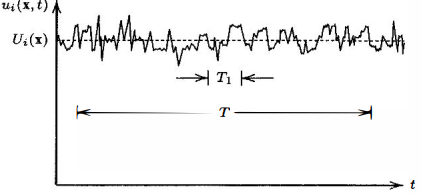
\includegraphics[width=0.5\textwidth]{foto01-decomposicao-reynolds.png}   
	\caption[Média temporal para turbulência estacionária para a velocidade instantânea \(u_i(\textbf{x},t)\).]{Média temporal para turbulência estacionária para a velocidade instantânea \(u_i(\textbf{x},t)\) \cite{Wilcox2006}.}
	\label{fig:decomposicao-reynolds}
\end{figure}

Como o foco da decomposição de Reynolds é resolver os problemas incompressíveis, as equações de Navier-Stokes para médias de Reynolds na forma conservativa são

\begin{gather}
	\label{eq:continuidade-decomposicao-reynolds}
	\frac{\partial U_i}{\partial x_i} = 0 \\
	\label{eq:momento-decomposicao-reynolds}
	\rho\frac{\partial}{\partial x_j}\left(U_{j}U_{i} + \overline{u'_j u'_i} \right) = -\frac{\partial P}{\partial x_i} + \frac{\partial}{\partial x_j}\left(2\mu S_{ji}\right)
\end{gather}
%
o termo \(S_{ij}\), presente na equação \ref{eq:momento-decomposicao-reynolds}, se trata do valor médio do tensor taxa de deformação, dado por

\begin{equation}
    \label{eq:tensor-medio-taxadeformacao}
    S_{ij} = \frac{1}{2}\left(\frac{\partial U_i}{\partial x_j} + \frac{\partial U_j}{\partial x_i} \right)
\end{equation}

O maior problema da turbulência é prescrever o termo \(\overline{u'_{i}u'_{j}}\), mas ao reescrever a equação \ref{eq:momento-decomposicao-reynolds} conforme a equação RANS padrão \cite{Wilcox2006}:

\begin{equation}
	\rho U_{j}\frac{\partial U_i}{\partial x_j} = -\frac{\partial P}{\partial x_i} + \frac{\partial}{\partial x_j}\left(2\mu S_{ji} - \rho\overline{u'_j u'_i} \right)
\end{equation}

A quantidade \(-\rho\overline{u'_{i}u'_{j}}\) é conhecido por tensor tensão de Reynolds, também escrito como \(\rho\tau_{ij}\), logo \(\tau_{ij}\) é o tensor tensão de Reynolds específico dado por

\begin{equation}
	\tau_{ij} = -\overline{u'_j u'_i}
\end{equation}
%
onde se verifica que é um tensor simétrico (\(\tau_{ij} = \tau_{ji}\)) com 6 variáveis independentes e desconhecidas. Por esta razão, é preciso encontrar mais equações para fechar o sistema, que já possui 4 variáveis a serem calculadas num escoamento tridimensional, o que implica em assumir 10 equações ao todo.

\subsection{Decomposição de Favre}

Nos escoamentos compressíveis as variações de densidade do fluido não são desprezíveis com o gradiente de pressão, permitindo criar novos termos para as equações de governo. Para solucionar este problema, deve-se aplicar as decomposições de Favre (ou pela médias das massas). O procedimento visto em seu trabalho afirma que a propriedade pode ser vista como uma média no tempo ponderada pela densidade, definida como a equação \ref{eq:densidade-decomposicao-favre}

\begin{equation} 
	\label{eq:densidade-decomposicao-favre}
    \rho = \overline{\rho} + \rho'
\end{equation}

Introduzindo a velocidade média pela massa, \(\Tilde{u}_i\), tem-se a equação \ref{eq:velocidade-decomposicao-favre}

\begin{equation}
	\label{eq:velocidade-decomposicao-favre}
	\Tilde{u_{i}} = \frac{1}{\overline{\rho}}\lim_{\tau \rightarrow \infty} \frac{1}{\tau}\int_{t}^{t+\tau}\rho(\textbf{x},t)u_i(\textbf{x},t)dt
\end{equation}
%
onde \(\overline{\rho}\) é a densidade média da decomposição de Reynolds. Dentre as propriedades mais relevantes para as equações de conservação, a decomposição de Favre resulta nas seguintes expressões:

\begin{equation}
\left. \begin{aligned}
  u_i &= \tilde{u}_i + u''_i \\
  p &= P + p' \\
  h &= \Tilde{h} + h'' \\
  e &= \Tilde{e} + e'' \\
  T &= \Tilde{T} + T'' \\
  q_j & = q_{L_j} + q'_j
\end{aligned}
\right\rbrace
\end{equation}
%
as notações com til (ex: \(\tilde{u}_i\)) são médias pelas densidade, enquanto que as variáveis com \(''\) (ex: \(u''_i\)) denotam as flutuações estatísticas geradas pelas médias de densidade. Logo abaixo estão as equações de governo para fluidos compressíveis de continuidade \ref{eq:continuidade-favre}, momento \ref{eq:momento-favre} e energia \ref{eq:energia-favre} que utilizam a decomposição de Favre \cite{Wilcox2006}:

\begin{gather}
    \label{eq:continuidade-favre}
    \frac{\partial}{\partial x_i} \left( \overline{\rho} \Tilde{u}_{i}\right) = 0 \\
    \label{eq:momento-favre}
    \frac{\partial}{\partial x_j} (\overline{\rho}\Tilde{u_i}\Tilde{u_j}) = -\frac{\partial P}{\partial x_i} + \frac{\partial}{\partial x_j}\left[\overline{t_{ji}} + \overline{\rho}\tau_{ji}\right] \\
    \label{eq:energia-favre} 
    \frac{\partial}{\partial x_j}(\overline{\rho} \Tilde{u_{j}} H) 
    = \frac{\partial}{\partial x_j}\left[-q_{L_{j}} - q_{T_{j}} + \overline{t_{ij}u''_i} - \overline{\rho u''_j\frac{1}{2}u''_i u''_i} \right] + \frac{\partial}{\partial x_j}\left[\Tilde{u_i}\left(\overline{t_{ij}} + \overline{\rho}\tau_{ij}\right)\right]
\end{gather}

Conforme nota-se ao longo do desenvolvimento das equações de Navier-Stokes, o termo P presente na equação \ref{eq:momento-favre} é a pressão corrigida para a decomposição de Favre, dada pela equação \ref{eq:pressao-favre}

\begin{equation}
	\label{eq:pressao-favre}
	P = \overline{\rho}R\Tilde{T}
\end{equation} 

Os termos \(E\) e \(H\) referem-se à energia total do sistema e a entalpia total do sistema, cujas equações demonstram ser funções da energia cinética turbulenta

\begin{equation}
	E = \Tilde{e} + \frac{1}{2}\Tilde{u_i}\Tilde{u_i} + \kappa 
	\hspace{0.5cm} 
	\text{e} 
	\hspace{0.5cm} 
	H = \Tilde{h} + \frac{1}{2}\Tilde{u_i}\Tilde{u_i} + \kappa
\end{equation} 

\subsubsection{Aproximações de Fechamento para os Escoamentos Compressíveis}

O fato de calcular as equações de Navier-Stokes a partir da decomposição de Favre resulta em resultados afetados pelos flutuações da densidade. Em qualquer modelo de transporte, aproximações de fechamento de caráter difusivo são normalmente postulados para as propriedades médias pela massa do tensor tensão de Reynolds e o vetor fluxo de calor \cite{Wilcox2006}. 

Para os modelos de zero até 2 equações, a hipótese de Boussinesq é uma razoável generalização dos escoamentos compressíveis, ou seja, o tensor tensão de Reynolds pela média das massas \(\rho\tau_{ij}\) e a viscosidade dinâmica turbulenta \(\mu_t\) é assumido da forma a seguir na equação \ref{eq:boussinesq-rans}

\begin{equation}
	\label{eq:boussinesq-rans}
	\rho\tau_{ij} \equiv \overline{-\rho u''_{i}u''_{j}} = 2\mu_t \left(S_{ij} - \frac{1}{3}\frac{\partial \Tilde{u}_k}{\partial x_k}\delta_{ij}\right) - \frac{2}{3}\overline{\rho}\kappa\delta_{ij}
\end{equation}

Outro termo que surgiu na equação \ref{eq:energia-favre} é o vetor fluxo turbulento de calor, \(q_{T_j}\), cuja aproximação para o fechamento foi proposta por Reynolds (1874), que assume ser proporcional ao gradiente médio de temperatura, como visto na equação \ref{eq:fluxo-turbulento-calor-reynolds} 

\begin{equation}
	\label{eq:fluxo-turbulento-calor-reynolds}
	q_{T_j} = \overline{\rho u''_j h''} = -\frac{\mu_t c_p}{Pr_t}\frac{\partial \tilde{T}}{\partial x_j} = -\frac{\mu_t}{Pr_t}\frac{\partial \tilde{h}}{\partial x_j}
\end{equation}
%
onde \(Pr_t\) é o número de Prandtl turbulento, que costuma ser aplicado como uma constante nos modelos RANS de turbulência \cite{Wilcox2006}.

\section{Modelo Spalart-Allmaras}

Esse modelo \cite{Spalart1992} envolve uma equação de transporte para a viscosidade cinética turbulenta \(\left(\nu_t\right)\). É amplamente utilizado em estudos sobre camadas-limites em projetos aerodinâmicos. O objetivo da aplicação deste modelo é possibilitar resultados prévios com alguma precisão ao menor custo computacional. Este método desejava remover as incompletudes dos modelos algébricos para cálculo da turbulência e, ao mesmo tempo, ser computacionalmente mais simples do que os modelos com duas equações \cite{pope_2000}. A viscosidade turbulenta é aplicada da forma vista na equação \ref{eq:visc-sa}:

\begin{equation}
    \label{eq:visc-sa}
    \nu_t = \Tilde{\nu} f_{\nu 1} \hspace{5mm} f_{\nu 1} = \frac{\chi^3}{\chi^3 + c^{3}_{\nu 1}} \hspace{5mm} \chi = \frac{\Tilde{\nu}}{\nu}
\end{equation}
%
e \(\Tilde{\nu}\) obedece a equação de transporte \ref{eq22:transport-sa}

\begin{equation}\label{eq22:transport-sa}
\begin{split}
    \frac{D\Tilde{\nu}}{Dt} &= c_{b1}[1 - f_{t2}]\Tilde{S}\Tilde{\nu} + \frac{1}{\sigma}\left[\nabla \cdot ((\nu + \Tilde{\nu})\nabla \Tilde{\nu}) + c_{b2}(\nabla \Tilde{\nu})^2 \right] \\&- \left[c_{w1}f_w - \frac{c_{b1}}{\kappa^2}f_{t2}\right]\left[\frac{\nu}{d}\right]^2 + f_{t1}\Delta U^2
\end{split}
\end{equation}

Considerando que

\begin{equation}
    \Tilde{S} \equiv S + \frac{\Tilde{\nu}}{\kappa^2d_{S-A}^2}f_{v2} \hspace{5mm} f_{v2} = 1 - \frac{\chi}{1 + \chi f_{v1}}
\end{equation}
%
onde \(S\) é a vorticidade e \(d_{S-A}\) a distância até a parede mais próxima para este modelo de turbulência. Já a função \(f_{w}\) é dada por

\begin{equation}
    f_w = g\left[\frac{1 + c^{6}_{w3}}{g^6 + c^{6}_{w3}} \right]^{1/6} \hspace{5mm} g = r + c_{w2}(r^6 - r) \hspace{5mm} r \equiv \frac{\Tilde{\nu}}{\Tilde{S}\kappa^2d^2}
\end{equation}

Pode-se assumir \(f_w = 10\) quando r é um valor grande. Enquanto isso, a função \(f_{t2}\) é dada por

\begin{equation}
    f_{t2} = c_{t3}\exp{(-c_{t4}\chi^2)}
\end{equation}

A última função \(f_{t1}\) que aparece na equação \ref{eq22:transport-sa} pode ser deduzida da forma a seguir:

\begin{equation}
    \label{eq:ft1-sa}
    f_{t1} = c_{t1}g_{t} \exp{\left(-c_{t2}\frac{\omega_{t}^{2}}{\Delta U^2}\left[d^{2} + g_{t}^{2}d_{t}^{2}\right]\right)} \hspace{5mm} g_t \equiv min(0,1, \Delta U/\omega_t \Delta x_t)
\end{equation}
%
onde \(\Delta x_t\) é o espaçamento ao longo da malha. As constantes utilizadas das equações \ref{eq:visc-sa} até \ref{eq:ft1-sa} podem ser vistas na Tabela \ref{tab:tabela-constantes-spalart-allmaras}. Os resultados obtidos mostraram a baixa influência da variação de densidade ao estudar os regimes supersônico \cite{Spalart1992}.

\begin{table}[ht]
\centering
\caption[Constantes usadas no modelo Spalart-Allmaras.]{Constantes usadas no modelo Spalart-Allmaras \cite{Spalart1992}}
\vspace{0.5cm}
\begin{tabular}{c|c}
 
Constante 		& Valor \\
\hline
\(c_{b1}\) 		& \num{0,1355} \\
\(\sigma\) 		& 2/3 \\
\(c_{b2}\) 		& \num{0,622} \\
\(\kappa\) 		& \num{0,41} \\
\(c_{w1}\) 		& \(c_{b1}/\kappa\) + (1 + \(c_{b2}\))/\(\sigma\) \\
\(c_{w2}\) 		& \num{0,3} \\
\(c_{w3}\) 		& \num{2,0} \\
\(c_{\nu 1}\) 	& \num{7,1} \\
\(c_{t1}\) 		& \num{1,0} \\
\(c_{t2}\) 		& \num{2,0} \\
\(c_{t3}\) 		& \num{1,2} \\
\(c_{t4}\) 		& \num{0,5} \\

\end{tabular}
\label{tab:tabela-constantes-spalart-allmaras}
\fonte{\cite{Spalart1992}}
\end{table}

\section{Modelo \texorpdfstring{\(\kappa-\varepsilon\)}{k-e} Padrão}

O modelo \(\kappa-\varepsilon\) \cite{JONES1972301,LAUNDER1974269,launder1974} apresenta uma forma de compreender a viscosidade turbulenta local através da energia cinética turbulenta, \(\kappa\), e pela taxa de dissipação dessa energia por unidade de massa, \(\varepsilon\). A viscosidade cinemática turbulenta, \(\nu_{t}\) é apresentada abaixo na equação \ref{eq:nut-k-epsilon}

\begin{equation}
    \nu_t = \frac{C_\mu k^2}{\varepsilon}
    \label{eq:nut-k-epsilon}
\end{equation}

Em altos números de Reynolds, as propriedades envolvidas possuem suas equações de transporte para a energia cinética turbulenta \ref{eq:transporte-k-modelo-k-epsilon} e para a taxa de dissipação específica \ref{eq:transporte-eps-modelo-k-epsilon} a serem resolvidas \cite{Wilcox2006}

\begin{gather}
    U_{j} \frac{\partial \kappa}{\partial x_j} = \tau_{ij}\frac{\partial U_i}{\partial x_j} - \varepsilon + \frac{\partial}{\partial x_j}\left[\left(\nu + \nu_{t}/\sigma_{\kappa}\right)\frac{\partial \kappa}{\partial x_j}\right]
    \label{eq:transporte-k-modelo-k-epsilon}
    \\
   	U_{j} \frac{\partial \varepsilon}{\partial x_j} = C_{1}\frac{\varepsilon}{\kappa}\tau_{ij}\frac{\partial U_i}{\partial x_j} - C_{2}\frac{\varepsilon^{2}}{\kappa} + \frac{\partial}{\partial x_j}\left[\left(\nu + \nu_{t}/\sigma_{\varepsilon}\right)\frac{\partial \varepsilon}{\partial x_j}\right]
    \label{eq:transporte-eps-modelo-k-epsilon}
\end{gather}
	
As constantes utilizadas neste método foram obtidas a partir de testes experimentais \cite{JONES1972301}, cujos resultados são apresentados na \autoref{tab:tabela-constantes-k-epsilon}. Embora o presente modelo seja bastante utilizado e obtenha bons resultados para escoamentos simples com gradientes de pressão considerados pequenos, o mesmo possui imprecisão nas proximidades de gradientes de pressão adversos \cite{Wilcox1988ReassessmentOT}. Portanto, há uma restrição deste modelo para análise de camada limite, a não ser que seja aplicado um tratamento para amortecer a viscosidade turbulenta nessa região em que o número de Reynolds é baixo \cite{Moukalled2015}.

\begin{table}[ht]
\centering
\caption[Constantes usadas no modelo \(\kappa-\varepsilon\).]{Constantes usadas no modelo \(\kappa-\varepsilon\) \cite{JONES1972301}}
\vspace{0.5cm}
\begin{tabular}{c|c}
 
Constante & Valor \\
\hline
\(C_{\mu}\) 				& \num{0,09} \\
\(C_{1}\) 					& \num{1,44} \\
\(C_{2}\) 					& \num{1,92} \\
\(\sigma_{k}\) 				& \num{1,0} \\
\(\sigma_{\varepsilon}\) 	& \num{1,3}

\end{tabular}
\label{tab:tabela-constantes-k-epsilon}
\fonte{\cite{JONES1972301}}
\end{table}

\section{Modelo \texorpdfstring{\(\kappa-\omega\)}{k-w} Padrão}

O modelo \(\kappa-\omega\) padrão \cite{Wilcox1988ReassessmentOT,Wilcox2006,Wilcox2008} constata as dificuldades do modelo \(\kappa-\varepsilon\) em predizer as camadas limites em gradientes adversos de pressão. A aplicação da lei da parede tende a esconder as imperfeições desses métodos. As análises feitas pelo desenvolvedor deste modelo permitiram-no concluir que a abordagem \(\kappa-\omega\) é satisfatória em escoamentos compressíveis, seja na camada limite ou em meio livre. Partindo da mesma sequência feita no modelo anterior, a viscosidade cinemática turbulenta, \(\nu_{t}\), é apresentada abaixo na equação \ref{eq:nu_t&kt_k-omega}.

\begin{equation}
    \nu_t = \frac{k}{\tilde{\omega}}
   	\hspace{1.0cm}
    \tilde{\omega} = \max{\left\lbrace \omega, C_{lim}\sqrt{\frac{2 S_{ij}S_{ij}}{\beta^*}}\right\rbrace}
    \hspace{1.0cm}
    C_{lim} = \frac{7}{8}
    \label{eq:nu_t&kt_k-omega}
\end{equation}

Mesmo sem fatores de amortecimento para a viscosidade turbulenta ou o uso da lei da parede, os resultados foram satisfatórios para estudos sobre a região da subcamada viscosa dentro da camada limite. Em adição aos fatos, os estudos também foram precisos em superfícies rugosas ou em escoamentos com adição de massa. Considerando \(\omega\) como a taxa específica de dissipação da energia, ela é definida pela equação \ref{eq:omega-k-omega}

\begin{equation}
	\label{eq:omega-k-omega}
	\omega = \frac{\varepsilon}{\beta^{*}\kappa}
\end{equation}

As vantagens de escolher esse modelo em vez do \(\kappa-\varepsilon\) padrão são \cite{Moukalled2015}:

\begin{enumerate}

	\item Mais robusto, por ser mais fácil de integrar numericamente;
	
	\item Pode ser integrado na região da subcamada limite viscosa sem aplicar funções de parede;

	\item Performa melhor com baixo gradiente adverso de pressão.
	
\end{enumerate}

As equações de transporte para a energia cinética turbulenta, \(\kappa\), \ref{eq:transporte-k-modelo-k-omega} e para a taxa específica de dissipação de energia, \(\omega\), \ref{eq:transporte-w-modelo-k-omega} são apresentadas abaixo \cite{Wilcox1988ReassessmentOT,Wilcox2006,Wilcox2008}

\begin{gather}
    \frac{\partial \rho u_{j}\kappa}{\partial x_j} = \rho\tau_{ij}\frac{\partial u_i}{\partial x_j} - \beta^{*}\rho\kappa\omega + \frac{\partial}{\partial x_j}\left[\left(\mu + \sigma^{*}\frac{\rho\kappa}{\omega}\right)\frac{\partial\kappa}{\partial x_j}\right]
    \label{eq:transporte-k-modelo-k-omega}
    \\
   	\frac{\partial\rho u_j\omega}{\partial x_j} = \alpha\frac{\omega}{\kappa}\rho\tau_{ij}\frac{\partial u_i}{\partial x_j} - \beta\rho\omega^{2} + \sigma_{d}\frac{\rho}{\omega}\frac{\partial\kappa}{\partial x_j}\frac{\partial\omega}{\partial x_j} + \frac{\partial}{\partial x_j}\left[\left(\mu + \sigma\frac{\rho\kappa}{\omega}\right)\frac{\partial\omega}{\partial x_j}\right]
    \label{eq:transporte-w-modelo-k-omega}
\end{gather}

As relações auxiliares para calcular o modelo são descritas a seguir:

\begin{equation}
\begin{aligned}
	\beta = \beta_{0}f_{\beta} 
	\hspace{1cm}
	\sigma_{d} =
	\begin{cases}
		0, &	\frac{\partial\kappa}{\partial x_j	}\frac{\partial \omega}{\partial x_j} \leq 0 \\
		\sigma_d, & \frac{\partial\kappa}{\partial x_j	}\frac{\partial \omega}{\partial x_j} > 0
	\end{cases}
	\hspace{1cm}
	f_{\beta} = \frac{1 + 85\chi_{\omega}}{1 + 100\chi_{\omega}} \\
	\chi_{\omega} \equiv \left|\frac{\Omega_{ij}\Omega_{ij}\hat{S}_{ki}}{(\beta^{*}\omega)^3}\right|
	\hspace{1cm}
	\Omega_{ij} = \frac{1}{2}\left(\frac{\partial U_i}{\partial x_j} - \frac{\partial U_j}{\partial x_i}\right)
	\hspace{1cm}
	\hat{S}_{ki} = S_{ki} - \frac{1}{2}\frac{\partial u_m}{\partial x_m}\delta_{ki}
\end{aligned}
\end{equation}

O maior contraponto a este modelo é a sensibilidade aos valores especificados para o escoamento livre \cite{Menter1992}, o que leva a forte dependência da solução arbitrária de \(\omega\) no meio livre, o que já não acontece no modelo \(\kappa-\varepsilon\). Os coeficientes utilizados no modelo \(\kappa-\omega\) são fornecidos na \autoref{tab:tabela-constantes-k-omega}

\begin{table}[ht]
\centering
\caption[Constantes usadas no modelo \(\kappa-\omega\).]{Constantes usadas no modelo \(\kappa-\omega\) \cite{Wilcox1988ReassessmentOT,Wilcox2006,Wilcox2008}.}
\vspace{0.5cm}
\begin{tabular}{c|c}
 
Constante & Valor \\
\hline
\(\alpha\) 		& \num{0,52} \\
\(\beta^*\) 	& \num{0,09} \\
\(\beta_{0}\) 	& \num{0,0708} \\
\(\sigma\) 		& \num{0,5} \\
\(\sigma^*\) 	& \num{0,6} \\
\(\sigma_{do}\) & \num{0,125}

\end{tabular}
\label{tab:tabela-constantes-k-omega}
\fonte{\cite{Wilcox1988ReassessmentOT,Wilcox2006,Wilcox2008}}
\end{table}

\section{Modelo \textit{Shear Stress Transport} \texorpdfstring{\(\kappa-\omega\)}{k-w}}

O modelo SST \(\kappa-\omega\) \cite{Menter1994TwoequationET,Menter2003,Menter2009} é baseado em duas equações para descrever a viscosidade turbulenta. Durante o desenvolvimento do modelo, muitos testes experimentais foram realizados, com ênfase em projetos aerodinâmicos. Foi proposto para as simulações de escoamentos aeronáuticos com altos gradientes adversos de pressão e separação de camada limite, por meio de uma combinação dos modelos \(\kappa-\varepsilon\) e \(\kappa-\omega\).

Com respeito a casos de escoamentos com camada limite, o modelo \(\kappa-\omega\) apresenta melhores resultados que o modelo \(\kappa-\varepsilon\) na solução da região viscosa próxima a parede, e seus resultados tem sido satisfatórios em casos que envolvem gradientes de pressão adversos. Entretanto, o modelo \(\kappa-\omega\) exige uma condição de contorno não nula para \(\omega\) para correntes livres não turbulentas, e o fluxo calculado apresenta elevada sensibilidade ao valor especificado \cite{Menter1994TwoequationET}. Foi demonstrado que o modelo \(\kappa-\varepsilon\) não apresenta essa deficiência \cite{Cazalbou1994}.

Logo, o modelo SST \(\kappa-\omega\) trata-se da combinação robusta e precisa do modelo \(\kappa-\omega\) na região próxima das paredes com a independência da corrente livre do modelo \(\kappa-\varepsilon\) fora da camada limite. Para isso, o modelo \(\kappa-\varepsilon\) é escrito em termos da taxa de dissipação específica, \(\omega\). Em seguida, o modelo \(\kappa-\omega\) padrão e o modelo \(\kappa-\varepsilon\) modificado são multiplicados por uma função de mistura e somados. As equações de transporte são desenvolvidas como a seguir em \ref{eq:transporte-k-modelo-sst-k-omega} e \ref{eq:transporte-w-modelo-sst-k-omega}.

\begin{gather}
    \frac{\partial}{\partial x_i}(\rho u_i \kappa) = \tilde{P}_\kappa - \beta^{*}\rho\kappa\omega + \frac{\partial}{\partial x_i}\left[(\mu + \sigma_{\kappa}\mu_t)\frac{\partial \kappa}{\partial x_i}\right]
    \label{eq:transporte-k-modelo-sst-k-omega}
    \\
   	\frac{\partial}{\partial x_i}(\rho u_i \omega)  = \alpha\frac{1}{\nu_t}\tilde{P}_\kappa - \beta\rho\omega^{2} + \frac{\partial}{\partial x_i}\left[(\mu + \sigma_{\omega}\mu_t)\frac{\partial \omega}{\partial x_i}\right] + 2(1 - F_1)\rho\sigma_{w2}\frac{1}{\omega}\frac{\partial\kappa}{\partial x_i}\frac{\partial \omega}{\partial x_i}
    \label{eq:transporte-w-modelo-sst-k-omega}
\end{gather}
%
cujos coeficientes dos modelos \(\kappa-\varepsilon\) e \(\kappa-\omega\) dependem da função de mistura \(F_1\), que é obtido pela equação \ref{eq:funcaomistura-modelo-sst-k-omega}

\begin{equation}
	\label{eq:funcaomistura-modelo-sst-k-omega}
    \tilde{\Gamma} = F_1 \Gamma_1 + (1 - F_1) \Gamma_2
\end{equation}
%
onde 

\begin{equation}
		F_1 = \tanh{(arg_1^{4})}
		\hspace{1cm}
    	arg_1 = \min\left[\max\left(\frac{\sqrt{\kappa}}{\beta^{*}\omega d(\perp)};\frac{500\nu}{d(\perp)^2 \omega}\right);\frac{4\rho\sigma_{\omega 2}\kappa}{CD_{k\omega}d(\perp)^2}\right]
\end{equation}
%
considere que d(\(\perp)\) é a distância perpendicular mais próxima à superfície e \(CD_{k\omega}\) é a parte positiva do termo de difusão cruzada.

\begin{equation}
    CD_{k\omega} = \max\left(2\rho\sigma_{\omega 2}\frac{1}{\omega}\frac{\partial \kappa}{\partial x_j}\frac{\partial \omega}{\partial x_j}, 10^{-10} \right)
\end{equation}

Neste modelo há uma correlação entre a energia cinética turbulenta e as tensões principais, \(\tau_{xy}\), conhecida como relação de Bradshaw, representada na equação \ref{eq:bradshaw-tensao-k} \cite{Menter1994TwoequationET}.

\begin{equation}
	\label{eq:bradshaw-tensao-k}
	\tau_{xy} = \mu_{t}\Omega = \rho\sqrt{\frac{\text{Produção de }\kappa}{\text{Dissipação de }\kappa}}a_{1}\kappa
\end{equation}

Assumindo que \(\Omega\) é a vorticidade, dada pela seguinte equação \ref{eq:vorticidade-modelo-sst-k-omega}.

\begin{equation}
	\label{eq:vorticidade-modelo-sst-k-omega}
	\Omega = \sqrt{2 S_{ij}S_{ij}}
\end{equation}

Para a viscosidade cinemática turbulenta, \(\nu_t\), a equação \ref{eq:visc-sst} é dada por

\begin{equation}
\begin{split}
    \label{eq:visc-sst}
    \nu_t = \frac{a_1 \kappa}{\max(a_1 \omega;\Omega F_2)} \hspace{1cm}
    F_2 = \tanh{\left(\max\left(2\frac{\sqrt{\kappa}}{\beta^{*}\omega d(\perp)}; \frac{500\nu}{ d(\perp)^2\omega}\right)^{2}\right)} 
\end{split}
\end{equation}
%
onde \(a_1 = 0,31\). O termo \(\tilde{P}_{\kappa}\) também significa a produção de energia cinética turbulenta, mas usada neste modelo para prevenir o crescimento da turbulência em regiões de estagnação \cite{Menter2009}. A equação \ref{eq:producao-tilde-k-modelo-sst-k-omega} se refere a esse ajuste do modelo SST \(\kappa-\omega\).

\begin{equation}
	\label{eq:producao-tilde-k-modelo-sst-k-omega}
	P_{\kappa} = \mu_{t}\frac{\partial u_i}{\partial x_j}\left(\frac{\partial u_i}{\partial x_j} + \frac{\partial u_j}{\partial x_i}\right)
	\hspace{1cm}
	\tilde{P}_{\kappa} = \min(P_\kappa, 10\cdot\beta^{*}\rho\kappa\omega)
\end{equation}

Houve uma ligeira alteração na primeira versão deste modelo RANS \cite{Menter1994TwoequationET}, pois o \(\tilde{P}_{\kappa}\) era proposto num fator de \num{20} em vez de \num{10}. A \autoref{tab:tabela-constantes-SST-k-omega} apresenta as constantes utilizadas para a formulação deste modelo de 2 equações:

\begin{table}[ht]
\centering
\caption[Constantes usadas no modelo SST \(\kappa-\omega\).]{Constantes usadas no modelo SST \(\kappa-\omega\) \cite{Menter1994TwoequationET,Menter2003,Menter2009}.}
\vspace{0.5cm}
\begin{tabular}{c|c|c|c}
 
Constante (\(\Gamma_1\)) 	& Valor  		 & Constante (\(\Gamma_2\)) & Valor \\
\hline
\(\alpha_1\) 				& \num{0,5532} 	 & \(\alpha_2\) 			& \num{0,4403} \\
\(\beta_1\) 				& \num{0,075}  	 & \(\beta_2\) 				& \num{0,0828} \\
\(\sigma_{\kappa 1}\) 		& \num{0,85}	 & \(\sigma_{\kappa 2}\) 	& \num{1,0} \\
\(\sigma_{\omega 1}\) 		& \num{0,50} 	 & \(\sigma_{\omega 2}\) 	& \num{0,856} \\
\(\beta^{*}\) 				& \num{0,09} 	 & \(\beta^{*}\) 			& \num{0,09} \\
\(k\) 						& \num{0,41} 	 & \(k\) 					& \num{0,41}

\end{tabular}
\label{tab:tabela-constantes-SST-k-omega}
\fonte{\cite{Menter1994TwoequationET,Menter2003,Menter2009}}
\end{table}

O modelo SST \(\kappa-\omega\) levou a uma grande melhoria, se comparado aos modelos \(\kappa-\omega\) e \(\kappa-\varepsilon\), para todos os escoamentos que envolvem gradientes adversos de pressão e \citeauthor{Menter1994TwoequationET} sugere que seja a técnica mais utilizada quando se trata de problemas de aerodinâmica. Outro fato importante é que nenhum outro método de duas equações para descrever a turbulência conseguiu predizer com acurácia a separação da pressão induzida e a interação viscosa-invíscida do escoamento.
\chapter{Modelo de Trajetória}\label{cap:trajetoria}
\graphicspath{{chapter-05/img-cap05/}}

Modelar uma trajetória para projetis estabilizados por rotação por ser uma tarefa complexa, principalmente pela obtenção de dados como o coeficiente de arrasto. A sugestão a seguir se propõe a reduzir os custos computacionais de modelos tradicionais como a dinâmica de corpo rígido em seis graus de liberdade \cite{McCoy2012}.

\section{Modelo de Trajetória Ponto-Material Modificado - MPMTM}
\label{subsec:MPMTM}

O modelo ponto-material modificado foi proposto por \citeauthor{Lieske1966} e revisto por \citeauthor{Baranowski2013-3}, sendo hoje um recurso disponível para os países membros da Organização do Tratado do Atlântico Norte (OTAN) \cite{stanag4355} por meio do acordo de padronização (STANAG) 4355, que analisa a dinâmica de voo através de 4 graus de liberdade, sendo três de translação e um por rotação. O objetivo deste modelo é oferecer um padrão a ser seguido para elaboração das tabelas de tiro dos projetis analisados \cite{McCoy2012,Carlucci2018}.

Neste modelo o corpo é tratado como um ponto material, embora haja estabilidade dinâmica a estudar. O grau de liberdade para a rotação pode ser chamado de "guinada de repouso", um método implícito para calcular todos os efeitos causados pelos momentos no corpo durante o voo. Neste trabalho serão consideradas as forças gravitacionais, o efeito de \textit{Coriolis} e as forças aerodinâmicas de arrasto, sustentação e \textit{Magnus}. Como pode ser percebido nas expressões a seguir, é um modelo altamente não-linear e há um grande acoplamento entre os movimentos translacionais e rotacionais:

\begin{equation}
    \label{eq:MPMTM - translation}
    \Sigma\boldsymbol{F} = m \dot{\boldsymbol{V}} = \boldsymbol{F}_{D} + \boldsymbol{F}_{G} + \boldsymbol{F}_{C} + \boldsymbol{F}_{L} + \boldsymbol{F}_{M} + \boldsymbol{F}_{BB}
\end{equation}

Para introduzir as descrições das forças na equação \ref{eq:MPMTM - translation}, é necessário frisar que as descrições seguintes das forças e das variáveis presentes que descrevem os movimentos translacional e rotacional advêm da norma proposta pela OTAN, isto é, respeitar um acordo que contempla toda a indústria de defesa e espaço.

Sobre a força gravitacional \(\boldsymbol{F}_{G}\) descreve a interação entre o corpo e o campo gravitacional da Terra, sendo igual ao produto da massa do projetil, m, com o vetor de aceleração pela gravidade, \(\boldsymbol{g}\), que pode ser vista na equação \ref{gravMPM}. O vetor \(\boldsymbol{g}\) considera o efeito da trajetória sobre uma aproximação esférica da Terra, bem como os efeitos de latitude. Tais questões são vistas nas equações \ref{eq:Gvec} e \ref{eq:Gmag}.

\begin{gather}
    \label{gravMPM}
    \boldsymbol{F}_{G} = -m\boldsymbol{g} \\
    \label{eq:Gvec}
    \boldsymbol{g} = -g_{0}\begin{bmatrix} 
        \frac{X}{R_{T}} \\
        1 - \frac{2Y}{R_{T}}\\
        \frac{Z}{R_{T}} \\
    \end{bmatrix} \\
    \label{eq:Gmag}
    g_{0} = \num{9,80665}[1 - \num{0,0026}cos(2lat)] 
\end{gather}
%
onde \(X\), \(Y\) e \(Z\) são as coordenadas cartesianas com o referencial inercial da Terra. Como já citado, a latitude, \(lat\), e o raio do planeta Terra, \(R_{T}\), influenciam a força causada pela gravidade.

O Efeito de Coriolis \(\boldsymbol{F}_{C}\) é usado em predições de trajetória, pois seu efeito é significativo em deslocamentos horizontais relativamente longos, algo em torno de 20 km \cite{McCoy2012}. Sua equação \ref{eq:corioMPM} é resultante da relação entre os efeitos de rotação da Terra em torno de seu próprio eixo e a velocidade de deslocamento do projetil em relação ao ar, de tal maneira que a aproximação esférica deste planeta também se faz presente por conta dos efeitos de latitude, \(\left(lat\right)\), e de azimute, \(\left(az\right)\), como descrito na equação \ref{eq:lambda}.

\begin{gather}
\label{eq:corioMPM}
\boldsymbol{F}_{C} = -m\boldsymbol{\Lambda} \\
\label{eq:lambda}
\boldsymbol{\Lambda} = 2\varphi
\begin{bmatrix} 
    -V_{y}cos(lat)cos(az) - V_{z}sin(lat) \\
    V_{x}cos(lat)sin(az) + V_{z}cos(lat)cos(az)\\
    V_{x}sin(lat) - V_{y}cos(lat)cos(az) \\
\end{bmatrix}
\end{gather}
%
onde \(V_{x}\), \(V_{y}\) e \(V_{z}\) são coordenadas da velocidade em relação ao ar, \(\boldsymbol{V}\). A constante \(\varphi\) = \qty{7,292e-5}{\radian\per\second} é a velocidade angular sobre seu próprio eixo polar.

A força de arrasto \(\boldsymbol{F}_{D}\) é a mais importante força aerodinâmica a ser calculada em um sistema de dinâmica de voo. Seu efeito é assunto de grande interesse pelas aplicações em extensão de alcance e otimização da dispersão. O arrasto pode ser representado pela equação \ref{eq:dragMPM}:

\begin{gather}
    \label{eq:dragMPM}
    \boldsymbol{F}_{D} = -\frac{\pi \rho D^{2}}{8} (C_{D_{0}} + C_{D_{\alpha^{2}}} [Q_{D}\alpha_{e}]^{2})V\boldsymbol{V}
\end{gather}
%
onde \(\rho\) é a densidade do ar, D é o diâmetro de referência do projetil, \(C_{D_{0}}\) é o coeficiente de arrasto aerodinâmico com ângulo de ataque nulo, \(C_{D_{\alpha^{2}}}\) é o coeficiente de arrasto aerodinâmico proporcional ao quadrado do ângulo de ataque, \(Q_{D}\) é uma constante que representa o fator de ajuste do arrasto em função do ângulo de ataque, \(\alpha_{e}\) é a magnitude da guinada de repouso, \(V\) é a magnitude da velocidade em respeito ao ar, e sua notação vetorial é reproduzida em \(\boldsymbol{V}\).

A força de sustentação \(\boldsymbol{F}_{L}\) age perpendicularmente ao voo, tendendo a ajustar o projetil na direção da ponta da ogiva \cite{McCoy2012}. Esta força é responsável por grande parte do deslocamento lateral. A equação \ref{eq:liftMPM} explica as variáveis envolvidas no processo.

\begin{equation}
    \label{eq:liftMPM}
    \boldsymbol{F}_{L} = \frac{\pi \rho D^{2} f_{L}}{8} (C_{L_{\alpha}}+C_{L_{\alpha^3}}\alpha_{e}^{2})V^{2} \boldsymbol{\alpha_{e}}
\end{equation}
%
onde \(C_{L\alpha}\) é o coeficiente de sustentação derivado do ângulo de ataque, \(C_{L\alpha^{3}}\) é o coeficiente de sustentação derivado do cubo do ângulo de ataque, \(f_{L}\) é o fator de sustentação e \(\boldsymbol{\alpha_{e}}\) é o vetor guinada de repouso.

A força de \textit{Magnus} \(\boldsymbol{F}_{M}\) é produzida através da diferença de pressão em lados opostos de corpos em rotação. Neste caso, a viscosidade do ar interage com a superfície girando, contudo esta força interfere muito menos no sistema, se comparada ao arrasto e ao efeito gravitacional. A equação \ref{eq:magnusMPM} expressa esse efeito: 

\begin{equation}
    \label{eq:magnusMPM}
    \boldsymbol{F}_{M} = -\frac{\pi \rho D^{3} Q_{M} \varrho C_{mag-f}}{8}(\boldsymbol{\alpha_{e}} \times \boldsymbol{V})
\end{equation}
%
onde \(C_{mag-f}\) é o coeficiente da força de Magnus, \(Q_{M}\) é a constante que representa o fator de ajuste da força de Magnus e \(\varrho\) é taxa de rotação axial do projetil.

Embora o Base Bleed não tenha por objetivo produzir força de empuxo, a equação \ref{eq:baseMPM} demonstra a força \(\textbf{F}_{BB}\) através do efeito causado pela injeção de gases na base do projetil, sempre na direção axial da trajetória. Este equacionamento permite entender como o alívio de pressão na base do projetil pode ser traduzido no movimento translacional.

\begin{equation} \label{eq:baseMPM}
    \boldsymbol{F}_{BB} = \frac{\pi \rho i_{BB} D^{2}}{8} f(Inj) C_{D_{BB}}V^{2} \left(\frac{\boldsymbol{V}cos(\alpha_{e})}{V} +\boldsymbol{\alpha_{e}}\right)
\end{equation}
%
\begin{equation}
f(Inj) =\begin{cases}
			\frac{Inj}{Inj_{0}}, & \text{se \(Inj < Inj_{0}\)}\\
            1, & \text{caso contrário}
		 \end{cases}
\end{equation}
%
onde \(C_{D_{BB}}\) é o coeficiente da força de arrasto produzida na base do equipamento; a variável \(i_{BB}\) é o fator de ajuste do arrasto em função do ângulo de elevação; \(f(Inj)\) é a função do parâmetro de injeção, \(Inj\), cujo objetivo é relacionar este parâmetro com o valor ótimo de injeção, \(Inj_{0}\) \cite{DAVENAS1993329}.

Em razão do movimento referencial e das condições atmosféricas que geram velocidades de vento, \(\boldsymbol{W}\), há uma diferença de velocidades em respeito ao solo, \(\boldsymbol{U}_{solo}\), e ao ar, \(\boldsymbol{V}\). Essa relação pode ser vista nas equações \ref{eq:Vvel} e \ref{eq:Vmag}.

\begin{gather}
    \label{eq:Vvel}
    V = |\boldsymbol{U}_{solo} - \boldsymbol{W}| \\ 
    \nonumber\\
    \label{eq:Vmag}
    V = \sqrt{(U_{x_{solo}}-W_{x})^2 + (U_{y_{solo}}-W_{y})^2 + (U_{z_{solo}}-W_{z})^2} \\
    \nonumber\\
    \label{eq:Uvec}
    \boldsymbol{U}_{solo} = \begin{bmatrix} 
        U_{disp}cos(QE)cos(az) \\
        U_{disp}sin(QE)\\
        U_{disp}cos(QE)sin(az) \\
    \end{bmatrix}
\end{gather}
%
onde a velocidade \(U_{disp}\) possui as condições iniciais de disparo, \(QE\) é igual ao ângulo de elevação do canhão e \(az\) representa o azimute de lançamento, sendo o ângulo nulo direcionado para o norte geográfico.

Como todo projetil que usa a tecnologia BB deve ser dinamicamente estabilizado pela rotação, \(\varrho\), a aceleração angular em torno de seu próprio eixo, \(\dot{\varrho}\), pode ser explicada pela equação \ref{eq:movimento-rotacao}, donde se deduz a rotação do projetil durante o voo.

\begin{equation}
    \label{eq:movimento-rotacao}
    \dot{\varrho} = \frac{\pi\rho D^{4}VC_{spin}\varrho}{8I_{x}} 
    \hspace{0.5cm}
    \varrho = \varrho_{0} + \int_{0}^{t}\dot{\varrho}dt 
    \hspace{0.5cm}
    \varrho_{0} = \frac{2\pi U_{disp}}{t_{c}D} 
\end{equation}
%
a condição inicial da rotação prevista em \(\varrho_{0}\) é calculada em função das características do canhão, como a taxa de torção, \(t_c\); do diâmetro de referência do projetil, \(D\), além da própria velocidade de disparo, \(U_{disp}\). A variável \(C_{spin}\) se refere ao coeficiente do momento de amortecimento da rotação (\textit{spin}).

A guinada de repouso \(\boldsymbol{\alpha}_{e}\) e os valores iniciais deste ângulo \(\boldsymbol{\alpha}_{e_{0}}\) são demonstrados na equação \ref{eq:guinada-de-reposicao}

\begin{equation}
	\label{eq:guinada-de-reposicao}
	 \boldsymbol{\alpha}_{e} = -\frac{8I_{x}\varrho(\boldsymbol{V}\times\dot{\boldsymbol{U}}_{solo})}{\rho\pi D^{3}(C_{m\alpha} + C_{m\alpha^{3}}\alpha_{e}^2)V^{4}}
	 \hspace{1cm}
	 \boldsymbol{\alpha}_{e_{0}} =
    \begin{bmatrix} 
        0 \\
        0 \\
        0 \\
    \end{bmatrix}
\end{equation}
%
onde \(C_{m_{\alpha}}\) and \(C_{m_{\alpha^3}}\) são, respectivamente, os coeficientes de momento de derrubada linear ao ângulo de ataque e proporcional ao cubo do ângulo de ataque.

\section{Modelo de Atmosfera}
\label{sec:ICAOatm}

Modelar as condições atmosféricas é de suma importância para cada problema que envolva sistemas dinâmicos de voo porque as forças aerodinâmicas são fortemente impactadas por elas. Por exemplo, a densidade atmosférica padrão proposta pela Organização Internacional de Aviação Civil (ICAO) \cite{international1993manual} na Troposfera (como também é conhecida a camada inferior da atmosfera) reduz-se em quase \qty{75}{\percent} conforme o projétil avance desde o solo até o valor limítrofe da camada, em torno de \qty{11}{\kilo\metre} de altura. Esse é um dos motivos que afetam diretamente a injeção de gases pelo gerador de \textit{Base Bleed}. Nesta convenção, o ar atmosférico é tratado como gás ideal nas camadas inferiores. 

\begin{equation}
\label{eq:funcoesICAO}
\begin{aligned}
p(Y) &=\begin{cases}
			p_{Y=\qty{0}{\metre}}\left[1 + \frac{\eta Y}{T(Y)} \right]^{\frac{-g_{0}}{\eta R}} , & Y \qty{< 11000}{\metre}\\
            p_{Y=\qty{11000}{\metre}} \exp\left[-\frac{g_{0}}{RT(Y)}(Y-\num{11000}) \right], & \qty{11000}{\metre} \leq Y \qty{< 20000}{\metre}
		 \end{cases}
\\
T(Y) &=\begin{cases}
			\num{288,15} + \eta Y, & Y < \qty{11000}{\metre}\\
            \num{216,15}, & \qty{11000}{\metre} \leq Y < \qty{20000}{\metre}
		 \end{cases}
\\
\rho &= \frac{p(Y)}{RT(Y)}
\end{aligned}
\end{equation}
%
onde \(\eta\) = \qty{6,5e-3}{\kelvin\per\metre} é igual ao gradiente de temperatura e R = \qty{287,05}{\joule\per\kelvin\per\kilogram} é a constante do ar com a massa molar de 28,97 kg/kmol. Deve-se atentar ao fato de que as funções presentes na equação \ref{eq:funcoesICAO} são dependentes do deslocamento vertical, Y. Outra propriedade importante para predizer a trajetória é a viscosidade dinâmica, \(\mu\). Pela lei de Sutherland, o valor local da viscosidade dinâmica é calculado em função da temperatura (em Kelvin) a certa altitude, \(T(Y)\), a partir da seguinte equação \ref{eq:sutherICAO}:

\begin{equation}
\label{eq:sutherICAO}
\mu = \frac{\beta_{S}T^{\frac{3}{2}}}{T + S}
\end{equation}
%
considere \(\beta_{S}\) = \qty{1,458e-6}{kg/(m.s.K^{1/2})} e S = \qty{110,4}{\kelvin} os valores para as constantes empíricas. Essa formulação ajuda a fechar as equações de Navier-Stokes, principalmente os casos compressíveis, assim como também permite determinar os coeficientes aerodinâmicos durante a trajetória a partir dos números de Reynolds, \(Re\) e de Mach, \(M\). Esses parâmetros adimensionais do escoamento podem ser vistos na equação a seguir:

\begin{equation}
    Re = \frac{\rho V D}{\mu} \hspace{1cm}
    M = \frac{V}{\sqrt{\gamma RT(Y)}}
\end{equation}
%
onde \(\gamma = c_{p}/c_{v}\) = 1,4 é a razão de expansão adiabática do ar como gas ideal monoatômico.
\section{Integração Numérica}
\label{sec:numint}

A solução numérica do modelo de trajetória de ponto-material modificado demanda certos recursos computacionais, o que significa que métodos de alta ordem precisam ser usados para resolver o problema. Uma boa aproximação dos resultados é usar o método Runge-Kutta de quarta-ordem (RK-4). Toda equação diferencial ordinária de primeira ordem pode ser expressa da seguinte forma \cite{ruggiero1996calculo}:

\begin{equation}
    \label{eq:rk4-pontoinicial}
    \frac{dy}{dx} = f(x,y)
\end{equation}

Todas as forças e a guinada de repouso são inclusas nesta equação \ref{eq:rk4-pontoinicial}, ainda que sejam equações não-lineares. Nesta situação, a variável independente da função é o tempo, o que é preferível do que usar coordenadas de deslocamento. O integrador numérico RK-4 usa a equação geral \ref{eq:rk4}:

\begin{equation}
    \label{eq:rk4}
    y_{i+1} = y_{i} + h_{RK4}\psi(x_{i},y_{i},h)
\end{equation}
%
cujo o subscrito \textbf{i} representa o índice do integrador, enquanto que x e y significam as variáveis dependentes a um i-ésimo tempo. A variável \(h_{RK4}\) é definida como o passo do integrador e \(\psi\) a função incremental, em outras palavras, uma função que ajusta \(f(x,y)\) de tal maneira que cubra toda a região da integral definida. Método RK-4 completo pode ser visto a seguir na equação \ref{eq:rk4-completo}.

\begin{equation}
    \label{eq:rk4-completo}
    y_{i+1} = y_{i} + \frac{h_{RK4}}{6}(k_{1}+2k_{2}+2k_{3}+k_{4})
\end{equation}
%
as notações \(\text{k}_{1}\), \(\text{k}_{2}\), \(\text{k}_{3}\), \(\text{k}_{4}\) são funções baseadas na função incremental, como as demonstrações feitas a seguir, das equações \ref{eq:k1} até \ref{eq:k4}:

\begin{subequations}\label{eq:rk4-termos-k1-ate-k4}
\begin{align}
    \label{eq:k1}
    k_{1} &= f(x_{i},y_{i}) \\
    \label{eq:k2}
    k_{2} &= f(x_{i}+\num{0,5}h_{RK4},y_{i}+\num{0,5}h_{RK4}k_{1}) \\
    \label{eq:k3}
    k_{3} &= f(x_{i}+\num{0,5}h_{RK4},y_{i}+\num{0,5}h_{RK4}k_{2}) \\
    \label{eq:k4}
    k_{4} &= f(x_{i}+\num{1,0}h_{RK4},y_{i}+\num{1,0}h_{RK4}k_{3}) 
\end{align}
\end{subequations}

Este método de integração precisa ser testado inúmeras vezes devido a influência do passo de tempo. Caso use um passo muito grande, os resultados possivelmente não estarão precisos. Todavia, usar pequenos intervalos de tempo requerem alto processamento de CPU, o que significa muitas horas para cada simulação.
\chapter{Descrição do Estudo Proposto}\label{cap:estudo-proposto}
\graphicspath{{chapter-06/img-cap06/}}

No presente trabalho serão ilustrados e analisados os resultados obtidos pelas análises numéricas computacionais para um escoamento compressível, axissimétrico e em regime permanente baseado na abordagem RANS para descrever a turbulência, em especial os modelos Spalart-Allmaras e SST $\kappa$-$\omega$. Dentre os trabalhos já citados, as referências \cite{Sahu1985,Mahmoud2009,torangatti2basawaraj,belaidouni2016,nicolas-perez_accuracy_2017,Dali2018a,Lucena2020,Reddy2021} serviram como norteadoras para o emprego dessas simulações. 

Ademais, a implementação do MPMTM faz uso dos recursos disponíveis pelas simulações CFD a fim de comparar o funcionamento do projetil em duas situações: o voo inerte, que seria o voo sem uso do \texit{Base Bleed}; voo ativo, com o uso do \texit{Base Bleed}. Desta forma, aplica-se o que já foi desenvolvido e consolidado em trabalhos anteriores \cite{Gauchoux1991,balon2006analysis,Abou-Elela2013,Skande2014,Lim2016,Rosendo2020}.

\section{Parâmetros de Interesse}

Nesta seção espera-se definir quais variáveis de saída são relevantes para o projeto. Por razões técnicas, a tecnologia \textit{Base Bleed} procura resolver o problema do arrasto induzido na base do projetil, logo são calculados os valores necessários para a compreensão desta força aerodinâmica. 

\subsection{Coeficiente de Arrasto}

Esse coeficiente ($C_D$) é um número adimensional que pode ser obtido de acordo com a equação \ref{eq:cd}:

\begin{equation} \label{eq:cd}
    C_{D} = \frac{F_{D}}{\frac{1}{2}\rho V^2 A}
\end{equation}
%
os termos $F_{D}$, $\frac{1}{2}\rho V^2$ e $A$ representam, respectivamente, a força de arrasto aerodinâmico, a pressão dinâmica exercida pelo fluido e a área de referência da munição. Neste trabalho em específico, não são considerados os efeitos causados pelo ângulo de ataque.

\subsection{Coeficiente de Pressão}

A pressão é uma das propriedades de maior interesse do fluido, portanto calcula-se um adimensional que permite entender como as forças de sustentação e arrasto se comportam no escoamento. O coeficiente de pressão ($C_{P}$) é um número adimensional que descreve as pressões relativas no escoamento independente do tamanho do corpo. Ele pode ser calculado a partir da expressão \eqref{eq:cp-equation}: 

\begin{equation}\label{eq:cp-equation}
    C_P = \frac{p - p_{\infty}}{\frac{1}{2}\rho_{\infty}V^2}
\end{equation}
%
onde $\text{p}_\infty$ e $\rho_\infty$ são, respectivamente, a pressão e a densidade do meio livre. Assume-se que quando os contornos de pressão indicam regiões com $C_{P} > 1$, o escoamento é compressível.

\subsection{Parâmetro de Injeção}

Para aplicar o conceito do parâmetro, $Inj$, é necessário olhar para a expressão \eqref{eq:parametro-injecao}:

\begin{equation}\label{eq:parametro-injecao}
    Inj = \frac{\Dot{m_{BB}}}{\rho_{\infty}u_{\infty}A_{b}}
\end{equation}
%
onde $\rho_{\infty}$ é a densidade do ar no meio livre; o $U_{\infty}$ é a velocidade do ar no meio livre e $A_{b}$ significa a área da base do projetil. 

Ao observar a equação anterior, o maior desafio é obter valores razoáveis para a injeção de gases na base do projetil. Para isto, deve-se ter em mãos os valores de vazão mássica do propelente injetado pelo sistema BB, $\Dot{m_{BB}}$. Como o fluido de trabalho para as simulações CFD é considerado ideal, portanto a vazão mássica pode ser calculada através da equação \ref{eq:vazao-massica-BB} \cite{Gil2020}:

\begin{equation}\label{eq:vazao-massica-BB}
    \Dot{m} = \rho_{t}A_{t}V_{t} = \frac{p_{c}A_{t}}{\sqrt{\gamma RT_{c}}}\sqrt{\frac{2\gamma^{2}}{\gamma - 1}\left(\frac{p_{t}}{p_{c}}\right)^{2/\gamma}\left[1-\left(\frac{p_{t}}{p_{c}}\right)^{(\gamma-1)/\gamma}\right]}
\end{equation}
%
Sejam $p_{c}$ e $p_{t}$ as pressões na câmara geradora de gás e na saída do sistema, respectivamente. Os termos $\rho_{t}$, $V_{t}$ e $A_{t}$ se referem a densidade, a velocidade e a área na saída do \texit{Base Bleed}. 

Como requisitos das simulações de dinâmica dos fluidos computacional, a temperatura e velocidade de saída dos gases (em função do número de Mach) são computadas com base na pressão da câmara, que é obtida a partir da equação para a vazão mássica \ref{eq:vazao-massica-BB}. Como o gás é isentrópico, as equações para essas propriedades são as seguintes:

\begin{align}
    \label{eq:temperatura-BB}
    T_{t} = T_{c}\left(\frac{p_t}{p_c}\right)^{(\gamma - 1)/\gamma} \\
    \label{eq:velocidade-mach-BB}
    M_{t} = \sqrt{\frac{2}{\gamma - 1}\left[\left(\frac{p_c}{p_t}\right)^{(\gamma - 1)/\gamma}-1\right]}
\end{align}

\section{Geração de malha}\label{sec:geracao-malha}

Para conseguir formular a abordagem numérica exigida pelo método de volumes finitos, a ser empregado no presente trabalho, foi necessário construir um domínio computacional através de uma malha. Com a evolução do projeto, foi construída um domínio axissimétrico em formato de "C", assim como visto em trabalhos anteriores \cite{Mahmoud2009,nicolas-perez_accuracy_2017}. Uma vantagem desse tipo de malha é permitir simplificações nas fronteiras para imposição das condições de contorno, além de reduzir o custo computacional para obtenção de resultados.

\begin{figure}[!ht]
	\centering
	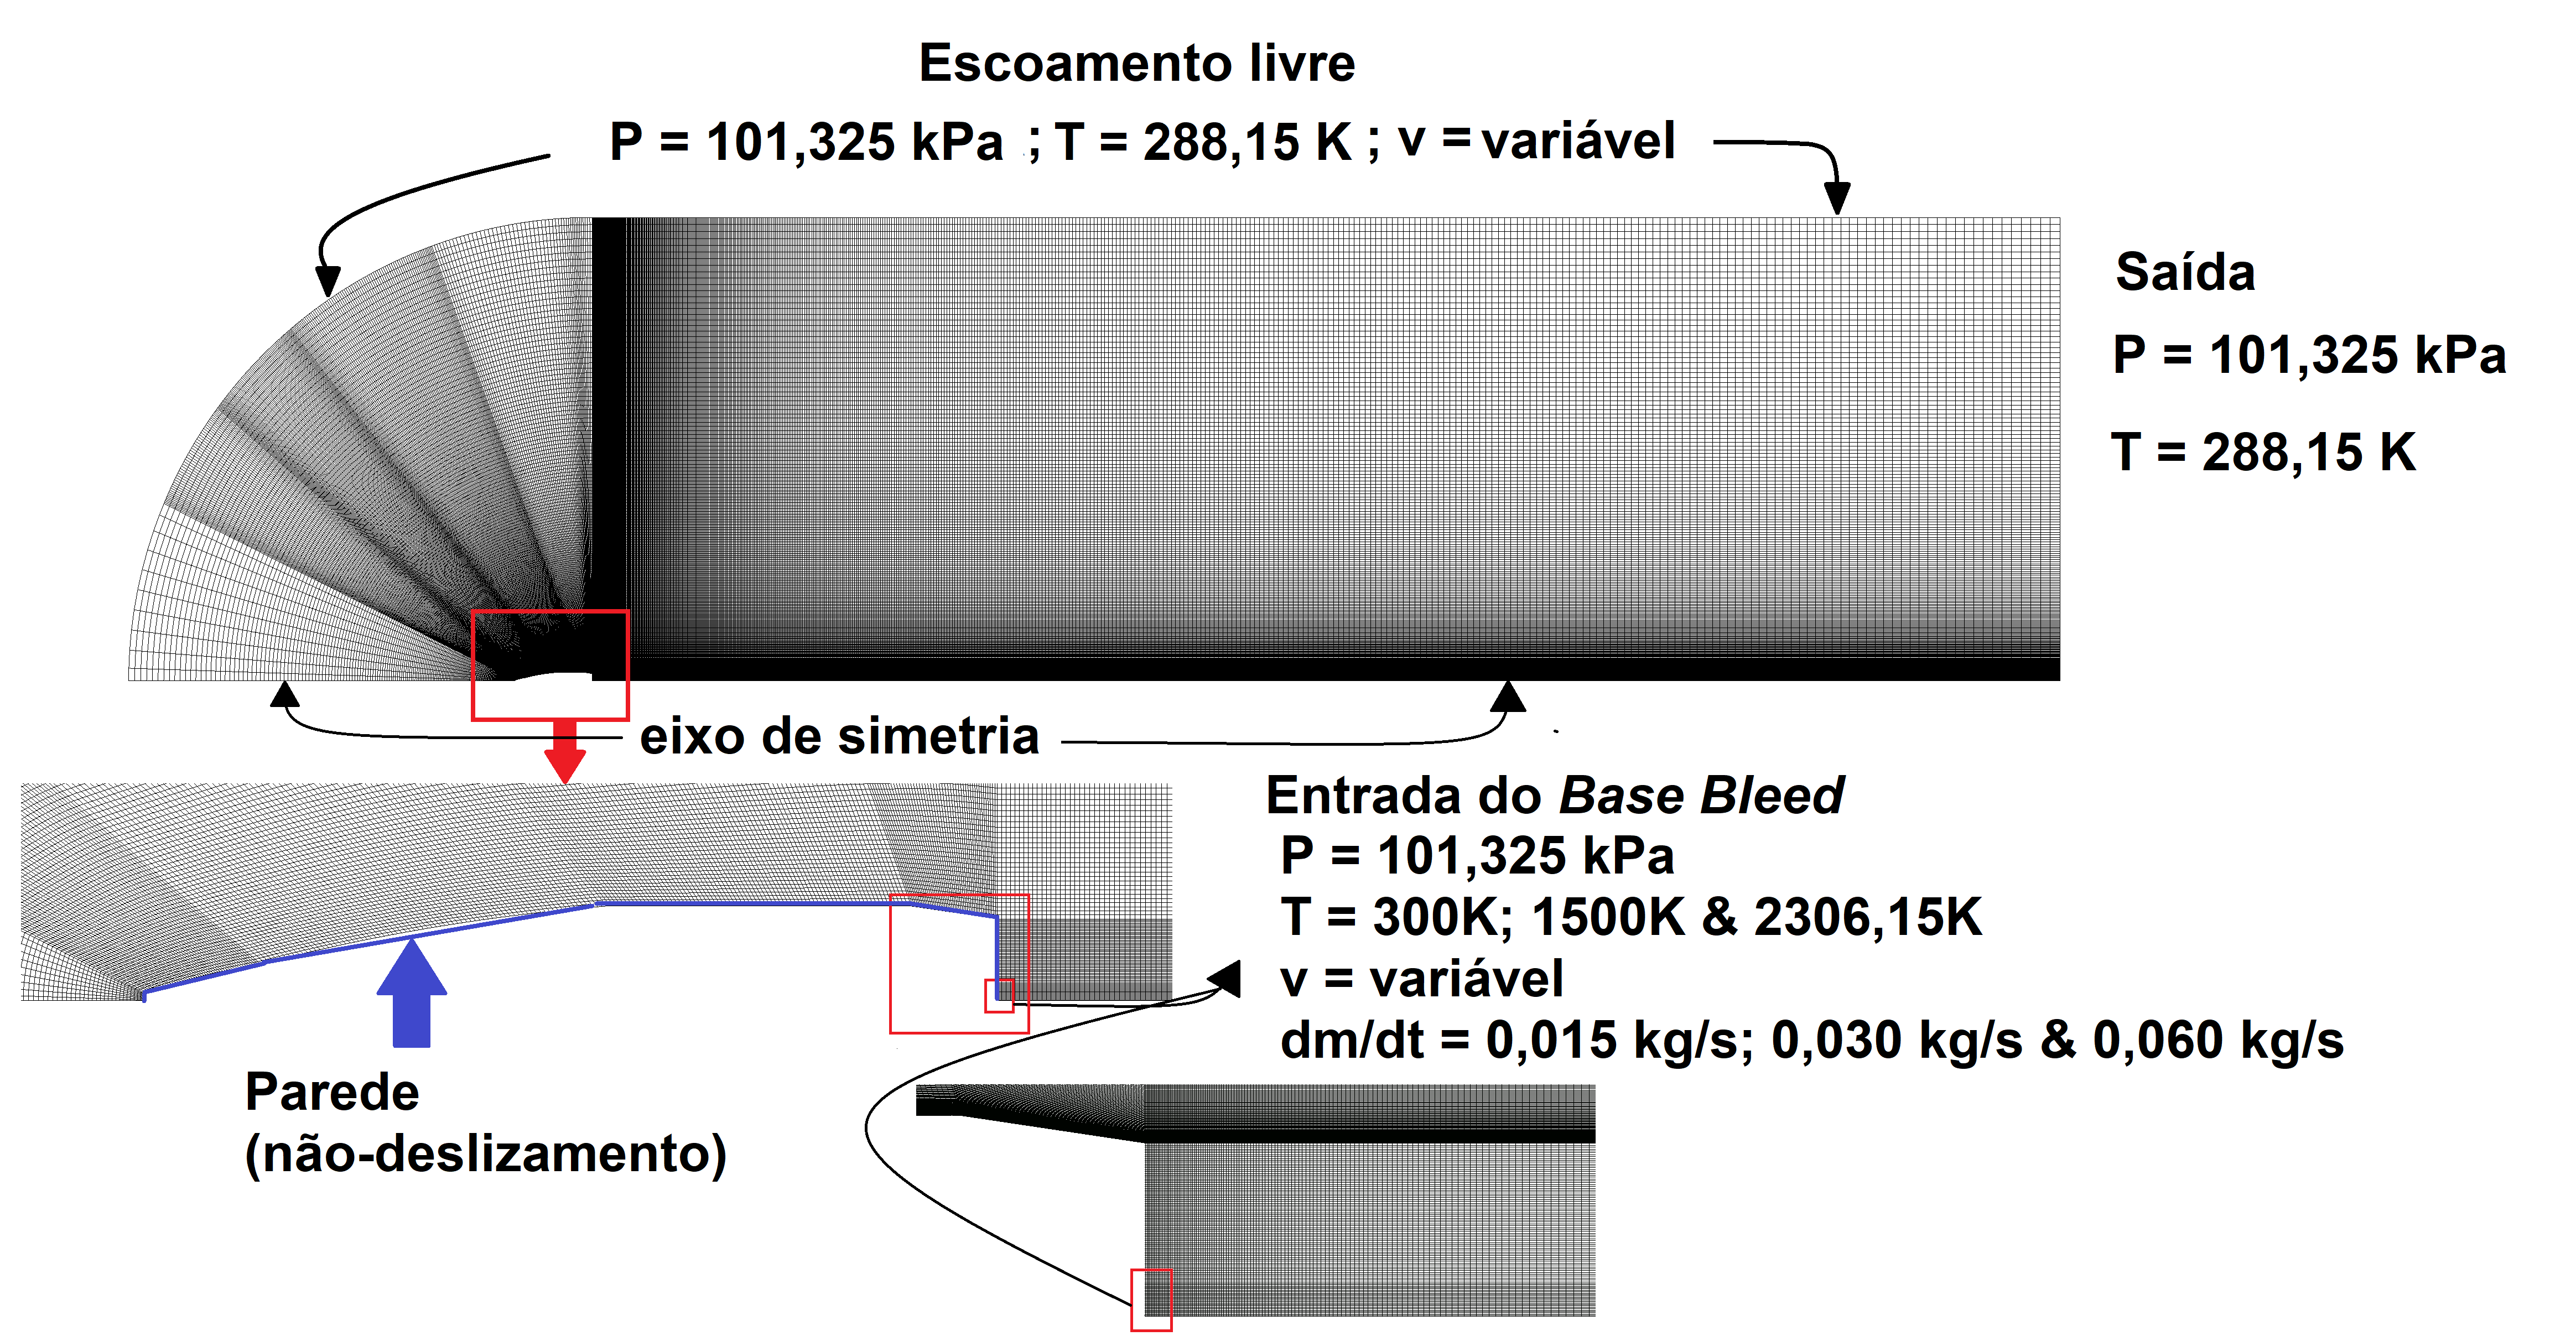
\includegraphics[width=1.0\textwidth]{foto01-malha.png}
	\caption{Domínio computacional}
	\label{fig12:autor-malha}
\end{figure}

E com o domínio preparado, foram feitas 2 malhas (vide \autoref{tab:tabela-malhas-inicial}), objetivando comparar valores com referências já citadas \cite{Mahmoud2009} para obter convergência dos resultados. Na direção vertical, a maior distância ao projetil é da ordem de 20 vezes o próprio calibre, enquanto que na direção horizontal à montante a maior distância ao projetil ficou na ordem de 5 vezes o comprimento longitudinal e à jusante na ordem de 15 vezes o valor do comprimento de referência da munição. Em ambos os casos, o diâmetro de saída do bocal do sistema \texit{Base Bleed} é de 1 polegada (25,4 mm).

\begin{table}[ht]
\centering
\caption[Malhas desenvolvidas para o domínio computacional (sem \textit{Base Bleed})]{Malhas desenvolvidas para o domínio computacional (sem \textit{Base Bleed})}
\vspace{0.5cm}
\begin{tabular}{c|c}
\multicolumn{2}{c}{Primeiro Teste de Convergência} \\
\hline 
Número da Malha & Quantidade de elementos \\ 
\hline
1 & 186500 \\
2 & 380000
\end{tabular}
\label{tab:tabela-malhas-inicial}
\fonte{Autor.}
\end{table}

A seguir a segunda fase de testes de convergência foi realizada, assumindo que o diâmetro de saída do bocal do sistema BB seja igual a 50,8mm e a temperatura de saída com valor de 2306,15K. Nesta etapa, foram testadas 4 malhas, de acordo com a \autoref{tab:tabela-malhas-secundaria}, com a finalidade era ratificar a suficiência da malha com 380000 elementos para obtenção dos resultados finais.

\begin{table}[ht]
\centering
\caption[Malhas desenvolvidas para o domínio computacional (com \texit{Base Bleed})]{Malhas desenvolvidas para o domínio computacional (com \textit{Base Bleed})}
\vspace{0.5cm}
\begin{tabular}{c|c}
\multicolumn{2}{c}{Segundo Teste de Convergência} \\
\hline 
Número da Malha & Quantidade de elementos \\ 
\hline
1 & 380000 \\
2 & 453600 \\
3 & 514800 \\
4 & 566550
\end{tabular}
\label{tab:tabela-malhas-secundaria}
\fonte{Autor.}
\end{table}

Após a ratificação dos valores encontrados para o coeficiente de arrasto, atestou-se a influência do efeito \texit{Base Bleed} pela temperatura de injeção dos gases. É importante salientar que a maior temperatura foi extraída de outro trabalho desenvolvido pelo autor desta dissertação em que se fez presente como co-autor \cite{Gil2020}.

\begin{table}[ht]
\centering
\caption[Efeito \textit{Base Bleed} em função da temperatura]{Efeito \texit{Base Bleed} em função da temperatura}
\vspace{0.5cm}
\begin{tabular}{c|c}
Diâmetro do Base Bleed (mm) & Temperatura (K)\\ 
\hline
\multirow{3}*{25,4} & 300\\
& 1500\\
& 2306,15
\end{tabular}
\label{tab:tabela-vazoes-por-diametro}
\fonte{Autor.}
\end{table}

Após esse passo, foram comparados dois diâmetros possíveis para saída da câmara geradora de gás (sistema BB) com a mesma temperatura, conforme a \autoref{tab:tabela-vazoes-por-diametro}.

\begin{table}[ht]
\centering
\caption[Diâmetros testados para analisar o efeito \textit{Base Bleed} ($T_{BB} = 2306,15 K$)]{Diâmetros testados para analisar o efeito \textit{Base Bleed} ($T_{BB} = 2306,15 K$)}
\vspace{0.5cm}
\begin{tabular}{c|c|c}
Diâmetro do \textit{Base Bleed} (mm) & Vazão nº1 (kg/s) & Vazão nº 2 (kg/s)\\ 
\hline
1" \hspace{2mm} 25,4 & 0,015 & 0,030\\
2" \hspace{2mm} 50,8 & 0,030 & 0,060
\end{tabular}
\label{tab:tabela-vazoes-por-diametro}
\fonte{Autor.}
\end{table}

\section{Condições Iniciais e de Contorno}\label{sec:condicao-contorno}

A região denominada "Entrada do \textit{Base Bleed}"{} (\textit{Base Bleed inlet}) mostrada na figura anterior representa a entrada de fluxo de gases injetados na base do projetil, onde a velocidade de entrada possui valor apenas na direção axial. A vazão mássica e a temperatura do BB foram impostas para descobrir a velocidade do escoamento nesta região, já que a pressão é definida a partir do gradiente nulo ($\nabla p = 0$) em respeito ao escoamento livre.

No local descrito como "Escoamento livre"{} (\textit{far-field}), o conceito por trás dessa condição é definir o meio livre do escoamento e, como requisito do software comercial utilizado, se fez necessário tratar o fluido (ar) como gás ideal. A pressão possui o valor de $1,01325 \times 10^{5}$ Pa (1 atm). A velocidade é prescrita conforme os valores de entrada do escoamento e a temperatura é determinada como $T = 288,15 \text{K}$ por razões de condições ambientais predeterminadas em tabelas de tiro.

No local descrito como "Saída"{} (\textit{outlet}) são prescritas apenas a pressão e a temperatura do contorno, que é igual ao valor encontrado no meio livre. A região da parede, que descreve o corpo sólido do projetil, possui a condição de não-deslizamento para desconsiderar o efeito dissipativo causado pela rugosidade da superfície. Há a referência para o eixo de simetria, a fim de se garantir que os cálculos sejam feitos de acordo com o estudo proposto. Em todas as regiões definidas o valor da intensidade de turbulência determinado é de 0\% e o comprimento da escala turbulenta igual a 0,7 metros, aproximadamente o valor do comprimento do projetil.

\section{Método de Resolução das Simulações CFD}\label{sec:metodo-resolucao-cfd}

Em todos os casos simulados no presente trabalho foi utilizado o método numérico denominado método dos volumes finitos \cite{McDonald1971,MacComarck&Paulay1972} para discretizar as equações de governo. O esquema de interpolação para os termos advectivos e difusivos foi o \textit{upwind} de $2^{a}$ ordem. 

Para lidar com a compressibilidade existente no regime de voo desta munição estudada, o esquema \textit{density-based} totalmente implícito foi aplicado \cite{Weiss1995PreconditioningAT,Weiss1997IMPLICITSO,Weiss1999ImplicitSO}.

Para o cálculo dos gradientes foi utilizado o método dos Mínimos Quadrados e o esquema de avaliação do fluxo optou pelo ROE-FDS, pois demonstra bons resultados para problemas com escoamentos compressíveis \cite{nicolas-perez_accuracy_2017}. Para a resolução do sistema de equações lineares foi utilizada a técnica \textit{multigrid} \cite{Hutchinson1986}.

O problema foi considerado convergido quando todos os resíduos forem menores que $1,0 \times 10^{-6}$. Um software comercial foi usado para a construção da geometria, construção das malhas, além de suporte aos métodos numéricos e equações de governo e no pós-processamento dos casos construídos \cite{fluent2021ansys}.

\section{Implementação do Modelo de Trajetória}\label{subsec:implementacao-trajetoria}

No trabalho de \citeauthor{Rosendo2020} cita-se a necessidade de dividir os dados de entrada relevantes de projeto em 4 grandes seções: aerodinâmicos, ambientais, balísticos e geométricos. Para maior esclarecimento, serão explicados nas subseções a posteriori.

\subsection{Condições Geométricas}\label{subsec:condicoes-geometricas}

O projetil de calibre 155mm possui um formato axissimétrico, portanto ele permite aplicar o modelo MPMTM. Isto é, o corpo rígido é tratado como um ponto material. Contudo, o \autoref{quad:geo_inputs} apresenta quais informações são exigidas para implementação do código que calcula a trajetória, conforme previsto pela STANAG 4355.

\begin{quadro}[htb]
\caption{\label{quad:geo_inputs}Dados Geométricos}
\begin{tabular}{|c|c|c|}
    \hline
    \textbf{Descrição} & \textbf{Valores} & \textbf{Unidade}\\ \hline
    Diâmetro de referência & 0,15470 & m\\ \hline
    Diâmetro do boat-tail & 0,13373 & m\\ \hline
    Massa (sem propelente) & 42,9850 & kg\\ \hline
    Massa do propelente & 0,5600 & kg\\ \hline
    Momento de inércia axial no início & 0,14245 & kg$\cdot$m$^{-2}$\\ \hline
    Momento de inércia axial após a queima & 0,13730 & kg$\cdot$m$^{-2}$\\\hline
    Centro de gravidade no início (a partir da ponta da ogiva) & 0,45835 & m\\\hline
    Centro de gravidade após a queima (a partir da ponta da ogiva) & 0,44645 & m\\\hline
\end{tabular}
\fonte{Autor.}
\end{quadro}

\subsection{Condições Balísticas}\label{subsec:condicoes-balisticas}

\begin{figure}[!ht]
	\centering
	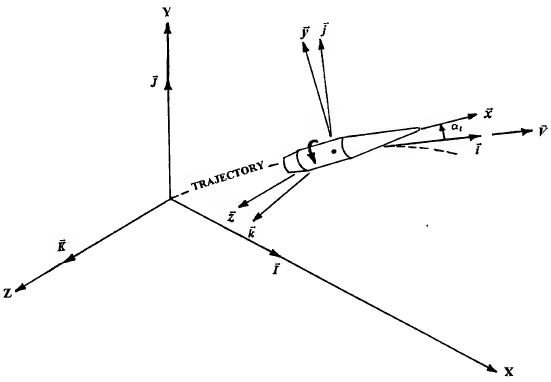
\includegraphics[width=0.5\textwidth]{foto02-mccoy2012.png}   
	\caption[Sistema de referência para o cálculo de trajetória]{Sistema de referência para o cálculo de trajetória \cite{McCoy2012}}
	\label{fig:traj-ref-mccoy2012}
\end{figure}

Neste sistema o canhão é centrado no eixo de referência da Terra em $O_{\text{XYZ}}$, conforme Figura \ref{fig:traj-ref-mccoy2012} e programado para lançar com ângulos de elevação de 40 e 45 graus a partir da horizontal, partindo com a mesma velocidade. Como citado na \autoref{quad:muzzle_inputs}, os fatores de arrasto e Magnus são constantes expressadas na STANAG 4355. A latitude do Rio de Janeiro foi considerada para vias de estudo.

\begin{quadro}[htb]
\caption{\label{quad:muzzle_inputs}Dados Balísticos}
\begin{tabular}{|c|c|c|}
\hline
\textbf{Descrição} & \textbf{Valores} & \textbf{Unidade}\\
\hline
Velocidade de disparo & 878 & m$\cdot$s$^{-1}$\\
\hline
Ângulo de elevação & $2\pi/9$, $\pi/4$ & radianos \\
\hline
Latitude & $-23 \pi/180$ & radianos \\
\hline
Azimute & 0 & radianos \\
\hline
Taxa de torção no disparo & 25 & calibres por revolução \\
\hline
Fator de arrasto & 1,2 & - \\
\hline
Fator de Magnus & 1,2 & - \\
\hline
\end{tabular}
\fonte{Autor.}
\end{quadro}

\subsection{Condições Ambientais}\label{subsec:condicoes-ambientais}

Respeitando o modelo da \citeonline{international1993manual}, existem algumas variáveis a saber no início do lançamento. Elas estão representadas no \autoref{quad:ICAOinputs}. A velocidade do vento foi desconsiderada porque o simulador necessitava criar confiabilidade antes de aumentar as incertezas, assim como os fatores de umidade foram desprezados pela mesma razão.

\begin{quadro}[htb]
\caption{\label{quad:ICAOinputs}Dados Atmosféricos}
\begin{tabular}{|c|c|c|}
\hline
\textbf{Descrição} & \textbf{Valores} & \textbf{Unidade}\\
\hline
Temperatura ao nível do mar & 288,15 & K\\
\hline
Gradiente de Temperatura & $6,5 \times 10^{-3}$ & K$\cdot$m$^{-1}$\\
\hline
Pressão do ar ao nível do mar & $1,01325 \times 10^{5}$ & Pa\\
\hline
Densidade do ar ao nível do mar & 1,225 & kg$\cdot$m$^{-2}$ \\
\hline
Razão de expansão adiabática do ar & 1,4 & - \\
\hline
Aceleração da gravidade ao nível do mar & 9,80665 & m$\cdot$s$^{-2}$\\
\hline
Raio da Terra & $6,371 \times 10^{6}$ & m\\
\hline
Velocidade angular da Terra & $7,292 \times 10^{-5}$ & rad$\cdot$s$^{-1}$ \\
\hline
\end{tabular}
\fonte{\citeonline{international1993manual}}
\end{quadro}

\subsection{Condições Aerodinâmicas}\label{subsec:condicoes-aerodinamicas}

Com o suporte do PRODAS®, os coeficientes aerodinâmicos foram calculados usando formulações semi-empíricas a partir das propriedades geométricas e de massa do projétil. Essas variáveis adimensionais são funções do número de Mach e da guinada de repouso de acordo com cada força atuante no sistema. Os coeficientes são todos em função de um projetil sem alcance estendido, pela limitação do software comercial. 

A norma faz uma comparação entre os coeficientes aerodinâmicos da STANAG 4355 com o que a NACA (Comitê Nacional para Aconselhamento da Aeronáutica) oferece \cite{stanag4355}. Por esta razão, os coeficientes obtidos no PRODAS® são calculados em função dos eixos da munição, enquanto que os valores adimensionais de interesse são em respeito ao vetor de velocidade do centro de massa. Por esta razão, são feitas algumas transformações rotacionais para se chegar nos coeficientes desejados:

\begin{align}
    C_{D_{0}} &= C_{X_{0}} \\
    C_{D_{\alpha^2}} &= C_{X_{\alpha^2}} + C_{Z_{\alpha}} - \frac{1}{2}C_{X_{0}}\\
    C_{L_{\alpha}} &= C_{Z_{\alpha}} - C_{X_{0}} \\
    C_{mag-f} &= \frac{1}{2}C_{y_{pa}} \\
    C_{spin} &= \frac{1}{2}C_{l_{p}}
\end{align}
%
os valores dos coeficientes que foram aplicados ao modelo de trajetória podem ser vistos do \autoref{apend:apendice-sembb} ao \autoref{apend:apendice-combb-2pol-006}.
\chapter{Resultados}\label{cap:resultados}
\graphicspath{{chapter-07/img-cap07/}}

\section{Projetil inerte (sem \textit{Base Bleed})}\label{sec:resultados-sem-basebleed}

Os valores encontrados para o coeficiente de arrasto aerodinâmico em um projetil de artilharia sem uso de \textit{Base Bleed} foram desenvolvidos a partir do modelo SST \(\kappa-\omega\), como visto na \autoref{fig:cd-sembasebleed-comparacao}. As curvas de arrasto foram desenvolvidas com base nas malhas citadas na \autoref{tab:tabela-malhas-inicial} e foram comparadas com os resultados obtidos em simulação computacional desenvolvida por \citeauthor{Mahmoud2009}. 

\begin{figure}[!ht]
	\centering
	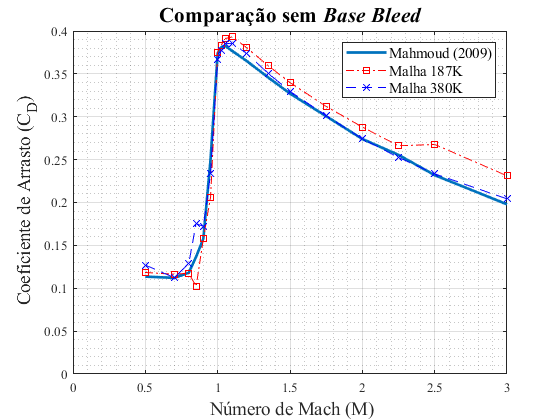
\includegraphics[width=0.75\textwidth]{cd-sembasebleed-comparacao.png}
	\caption{Coeficiente de Arrasto \(C_{D}\) em função do número de Mach (sem BB)}
	\label{fig:cd-sembasebleed-comparacao}
\end{figure}

Através do que é demonstrado na Figura \autoref{fig:cd-sembasebleed-comparacao}, percebe-se que a curva referente a malha com \num{380000} elementos (380K) se aproximou consideravelmente da referência. Por esta razão, a implementação do domínio computacional foi considerada válida para as próximas análises com a tecnologia \textit{Base Bleed} como condição de contorno.

\begin{figure}[!ht]
	\centering
	\begin{subfigure}[b]{0.47\textwidth}
        \centering
        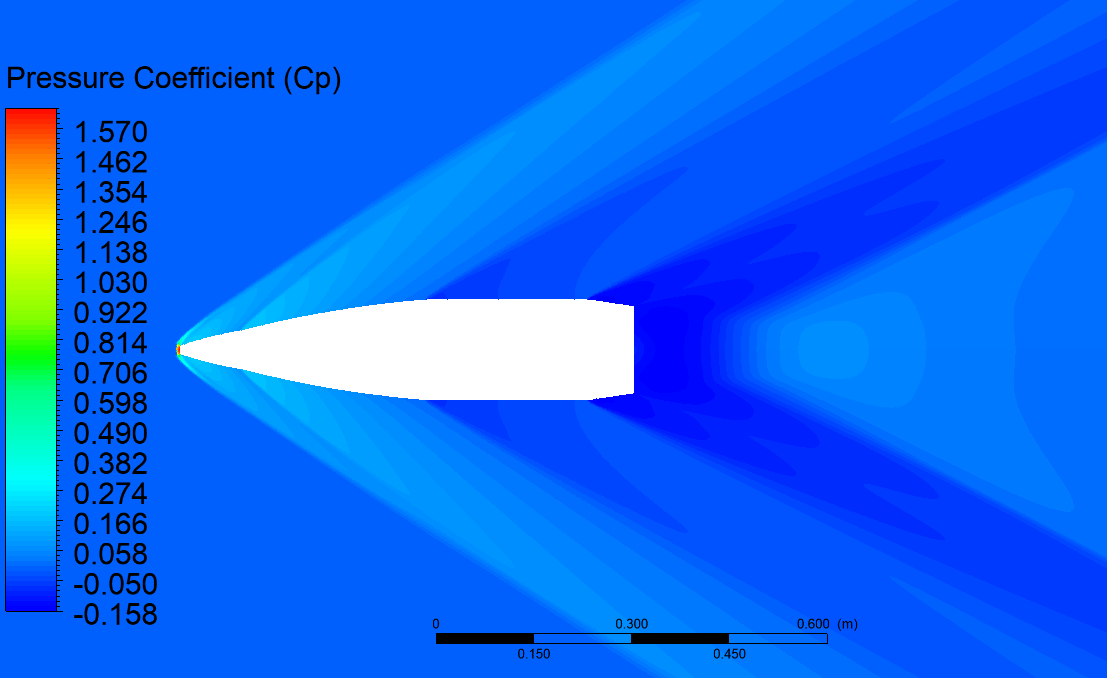
\includegraphics[height=5cm,width=\textwidth]{contorno-pressao.png}
        \caption{Contornos de Pressão}
        \label{fig:contorno-pressao-sembasebleed}
    \end{subfigure}
    \hfill
	\begin{subfigure}[b]{0.47\textwidth}
        \centering
        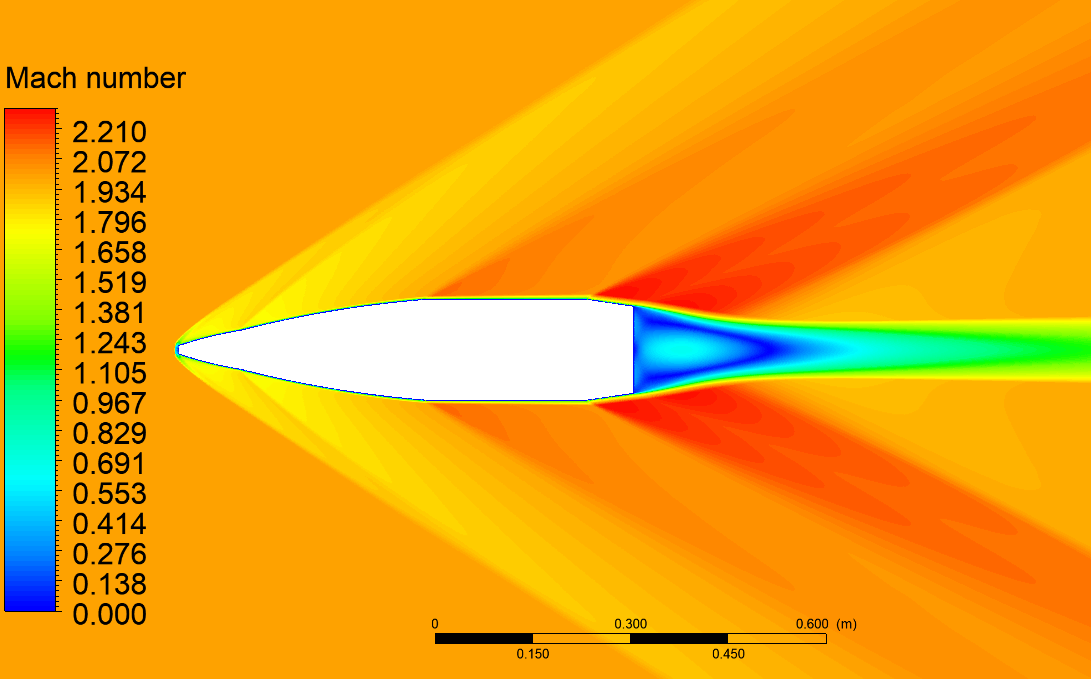
\includegraphics[height=5cm,width=\textwidth]{contorno-velocidade.png}
        \caption{Contornos de Velocidade}
        \label{fig:contorno-velocidade-sembasebleed}
    \end{subfigure}
	\caption{Projetil sob regime de velocidade igual a Mach \num{2}}
	\label{fig:contornos-pressao-velocidade-sembasebleed}
\end{figure}

Antes de iniciar as validações das simulações que incluem o efeito \textit{Base Bleed}, é necessário observar a \autoref{fig:contornos-pressao-velocidade-sembasebleed}, pois os contornos de pressão (\autoref{fig:contorno-pressao-sembasebleed}) e de velocidade (\autoref{fig:contorno-velocidade-sembasebleed}) demonstram o escoamento do ar em torno do projetil. Além da onda de choque causada pela velocidade supersônica (M = \num{2,0}), existe uma região de baixa pressão na base da munição cuja consequência é criar uma região de recirculação com baixas velocidades. Contudo, é a partir da \autoref{fig:corrente-velocidade-sembasebleed} que se examina com maiores detalhes o comportamento desta recirculação outrora citada.

\begin{figure}[!ht]
    \centering
    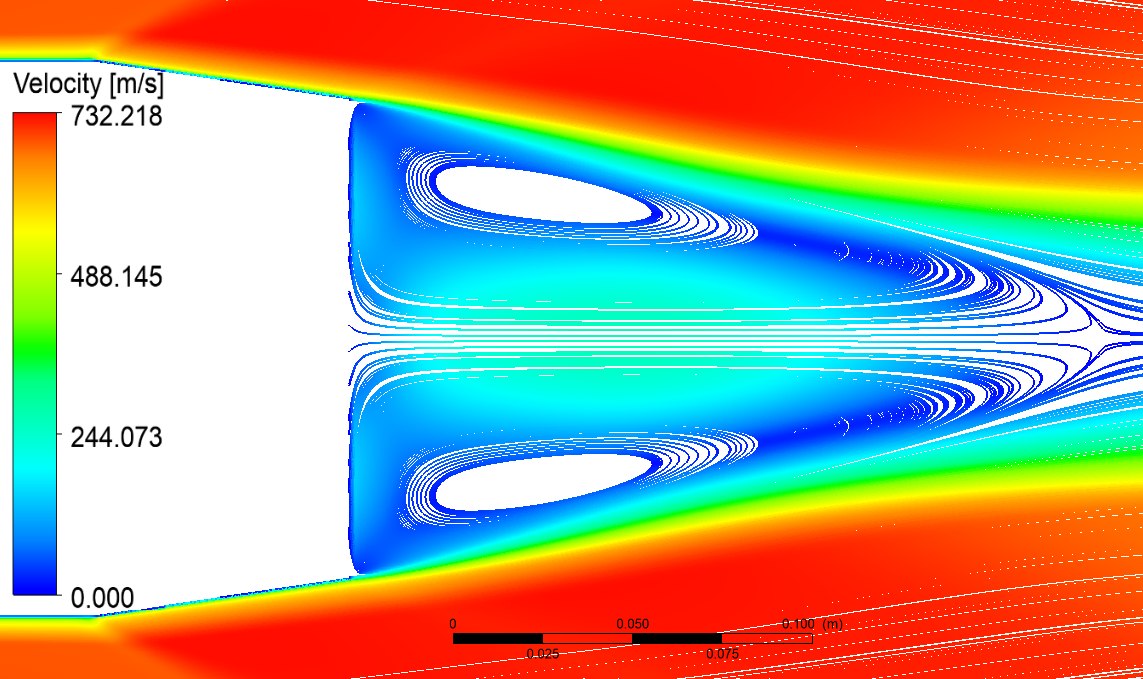
\includegraphics[height=5cm,width=0.5\textwidth]{corrente-velocidade-off.png}
    \caption{Linhas de corrente para a velocidade sob regime M = \num{2,0}}
    \label{fig:corrente-velocidade-sembasebleed}
\end{figure}

\section{Projetil ativo (com \textit{Base Bleed})}\label{sec:resultados-com-basebleed}

A Tabela \ref{tab:tabela-malhas-secundaria}, presente na Seção \ref{sec:geracao-malha}, demonstra as malhas testadas para o projetil ativo. A malha com \num{380000} elementos foi utilizada como referência, tendo em vista a convergência dos resultados com valores de trabalhos anteriores \cite{Mahmoud2009}. Com estas malhas foram feitos testes de convergência, em dois regimes de velocidade (Mach igual a \numlist{1,0;2,0}), cujos resultados são apresentados na \autoref{tab:tabela-malhas-convergencia}. Em ambos os casos o modelo SST \(\kappa-\omega\) foi usado para descrever a turbulência. A condição de contorno "Entrada do \textit{Base Bleed}"{} considerou a saída dos gases com a seguinte configuração: \(\phi_{BB} = \qty{50,8}{\milli\metre}; \Dot{m}_{BB} = \qty{0,030}{\kilogram\per\second}; T_{BB} = \qty{2306,15}{\kelvin}\).

\begin{table}[ht]
\centering
\caption[Teste de convergência (com \textit{Base Bleed})]{Teste de convergência (com \textit{Base Bleed})}
\vspace{0.5cm}
\begin{tabular}{c|c|c|c|c}
\multicolumn{5}{c}{Segundo Teste de Convergência} \\
\hline 
Número de elementos & \(C_{D}\) (M = \num{1}) & Diferença & \(C_{D}\) (M = \num{2}) & Diferença\\ 
\hline
\num{380000} & 0,32784 & -- & 0,26330 & --\\
\num{453600} & 0,33064 & \qty{0,854}{\percent} & 0,26364 & \qty{0,129}{\percent}\\
\num{514800} & 0,32912 & \qty{0,390}{\percent} & 0,26185 & \qty{0,551}{\percent}\\
\num{566550} & 0,32656 & \qty{0,394}{\percent} & 0,26143 & \qty{0,710}{\percent}\\
\end{tabular}
\label{tab:tabela-malhas-convergencia}
\fonte{Autor.}
\end{table}

Para o projetil em velocidade sônica (M = \num{1,0}), a maior diferença percentual ficou na ordem de \qty{0,85}{\percent}, enquanto que para M = \num{2,0} o maior desvio foi de aproximadamente \qty{0,7}{\percent}, o que denota quase nenhuma diferença nos resultados mesmo aumentando significativamente o número de elementos. Desta forma, o custo computacional para resolver a malha com \num{380000} elementos é suficiente para predizer o coeficiente de arrasto.

\subsection{Influência no diâmetro de saída do \textit{Base Bleed}} \label{subsec:resultados-com-basebleed-diametros}

Outro parâmetro considerado foi o aumento do diâmetro da saída do bocal (ver \autoref{tab:tabela-vazoes-por-diametro}), de \qtyrange{25,4}{50,8}{\millimetre} (de \qtyrange{1}{2}{\polegada}). A temperatura na condição de contorno "Entrada do \textit{Base Bleed}"{} foi fixada em \(T_{BB} = \qty{2306,15}{\kelvin}\). Desta forma, a Figura \ref{fig:comparacao-bb-diametro-2pol} demonstra uma redução do coeficiente de arrasto para um diâmetro de \qty{2}{\polegada}, enquanto que a Figura \ref{fig:comparacao-bb-diametro-1pol} mostrou que o diâmetro de \qty{1}{\polegada} aumentou o perfil de arrasto, se comparado ao sistema BB desativado.

\begin{figure}[!ht]
	\centering
	\begin{subfigure}[b]{0.47\textwidth}
    	\centering
    	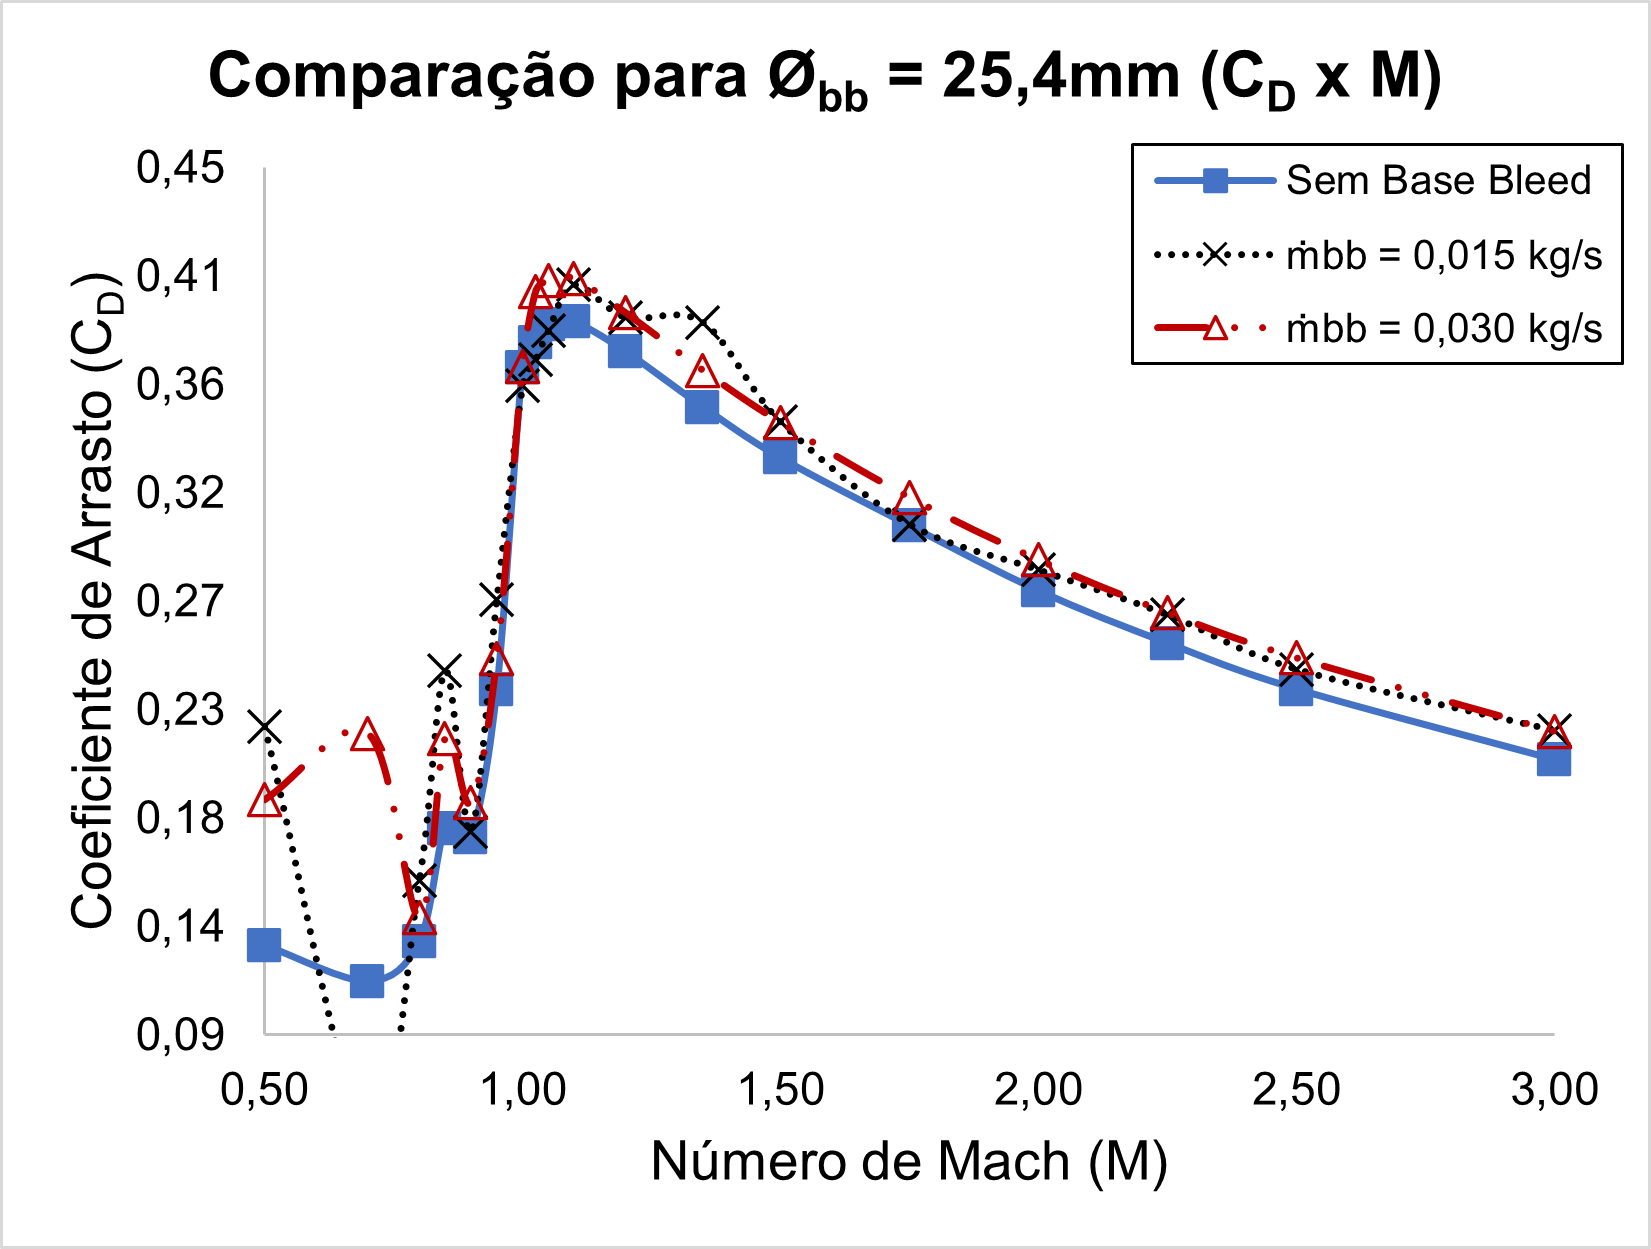
\includegraphics[width=\textwidth]{cd-combasebleed-diametro-1pol.png}
    	\caption{Saída do bocal - \(\phi_{BB}\) = \qty{25,4}{\millimetre}}
    	\label{fig:comparacao-bb-diametro-1pol}
    \end{subfigure}
    \hfill
	\begin{subfigure}[b]{0.47\textwidth}
    	\centering
    	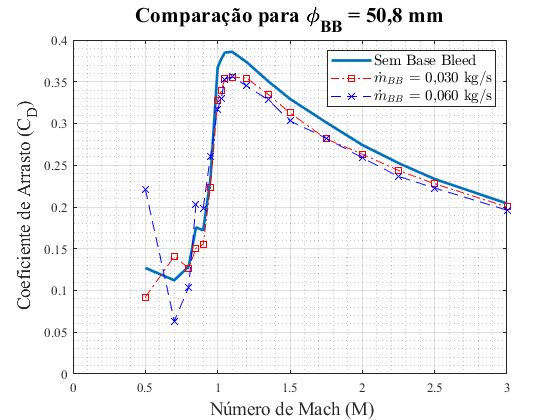
\includegraphics[width=\textwidth]{cd-combasebleed-diametro-2pol.png}
    	\caption{Saída do bocal - \(\phi_{BB}\) = \qty{50,8}{\millimetre}}
    	\label{fig:comparacao-bb-diametro-2pol}
    \end{subfigure}
	\caption{Influência do diâmetro sobre o coeficiente de arrasto.}
	\label{fig:comparacao-bb-diametro-vazoes}
\end{figure}

Há de se notar uma oscilação presente nas curvas de arrasto no regime subsônico com o \textit{base bleed} funcionando, especialmente na faixa M < \num{0,8}. A escolha das vazões de \qty{0,015}{\kilogram\per\second} e \qty{0,060}{\kilogram\per\second} foi para garantir a conservação da velocidade ao aumentar em 4 vezes a área de saída dos gases do \textit{Base Bleed}. Ainda analisando os resultados pelas vazões mássicas, atesta-se da \autoref{fig:comparacao-bb-diametro-vazoes} que os coeficientes de arrasto sofreram redução em ambos os casos, embora pouco relevantes.

Para entender o que ocorreu para acrescentar o arrasto nos projetis com diâmetro de saída do \textit{Base Bleed} iguais a \qty{1}{"} \(\left(\phi_{BB} = \qty{25,4}{\millimetre}\right)\), a \autoref{fig:influencia-diametro-vazao-1pol} apresenta os campos de pressão e velocidade sob regime M = \num{2,0}. Conforme esperado pela literatura, as Figuras \ref{fig:contorno-pressao-bb-1pol-vazao0015} e \ref{fig:contorno-pressao-bb-1pol-vazao0030} demonstram o campo de pressão à jusante da base do projetil, que está abaixo do valor prescrito da região denominada "Escoamento livre"{} do domínio computacional. Tanto na \autoref{fig:contorno-pressao-bb-1pol-vazao0015} quanto na \autoref{fig:contorno-pressao-bb-1pol-vazao0030} não há um aumento significativo da pressão atmosférica na região, apesar da diferenciação do campo de velocidades ser demonstrada pelas Figuras \ref{fig:contorno-velocidade-bb-1pol-vazao0015} e \ref{fig:contorno-velocidade-bb-1pol-vazao0030}. Contudo, a apresentação do campo de velocidades da \autoref{fig:contorno-velocidade-bb-1pol-vazao0030} reflete uma vazão mássica excedente que aumenta a força de arrasto.

As Figuras \ref{fig:corrente-velocidade-bb-1pol-vazao0015} e \ref{fig:corrente-velocidade-bb-1pol-vazao0030} mostram as linhas de corrente para a velocidade nas duas condições impostas para o sistema BB com \qty{1}{\polegada}. Da \autoref{fig:corrente-velocidade-bb-1pol-vazao0015} se conclui que a injeção de gases nessa vazão mássica produz nenhum efeito significativo no que diz respeito ao deslocamento da região primária de recirculação e da formação da recirculação anular.

\begin{figure}[!ht]
	\centering
	\begin{subfigure}[b]{0.47\textwidth}
        \centering
        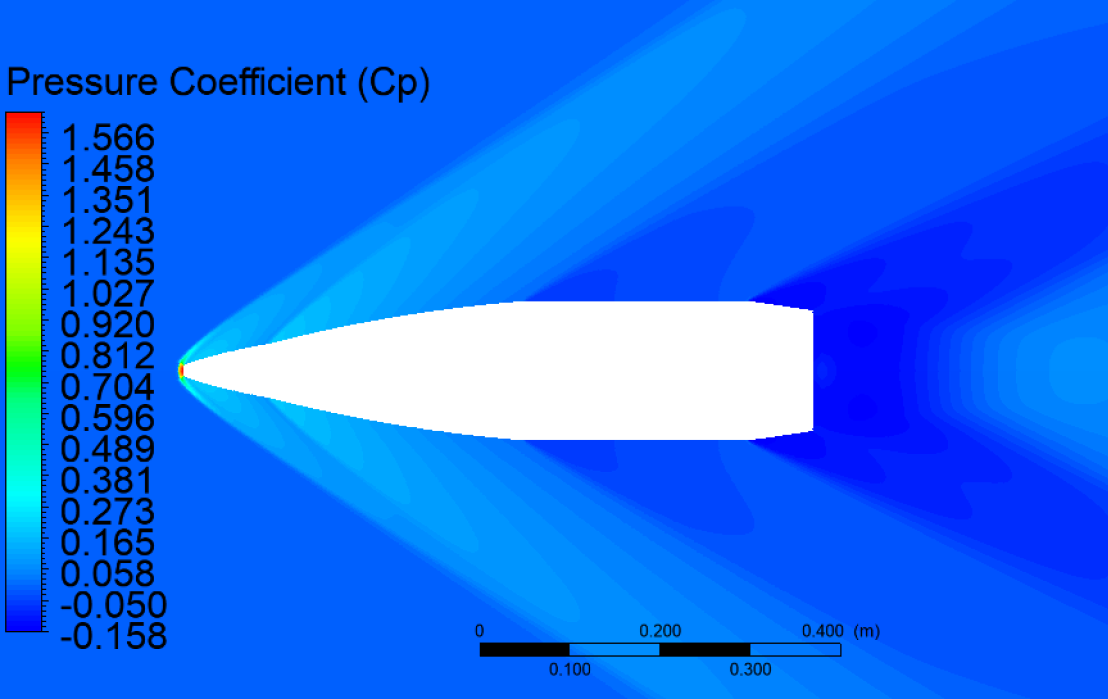
\includegraphics[height=5cm,width=\textwidth]{contorno-pressao-2306K-vazao-0015-1pol.png}
        \caption{Contornos de Pressão - \(\Dot{m}_{BB}\) = \qty{0,015}{\kilogram\per\second}}
        \label{fig:contorno-pressao-bb-1pol-vazao0015}
    \end{subfigure}
    \hfill
    \begin{subfigure}[b]{0.47\textwidth}
        \centering
        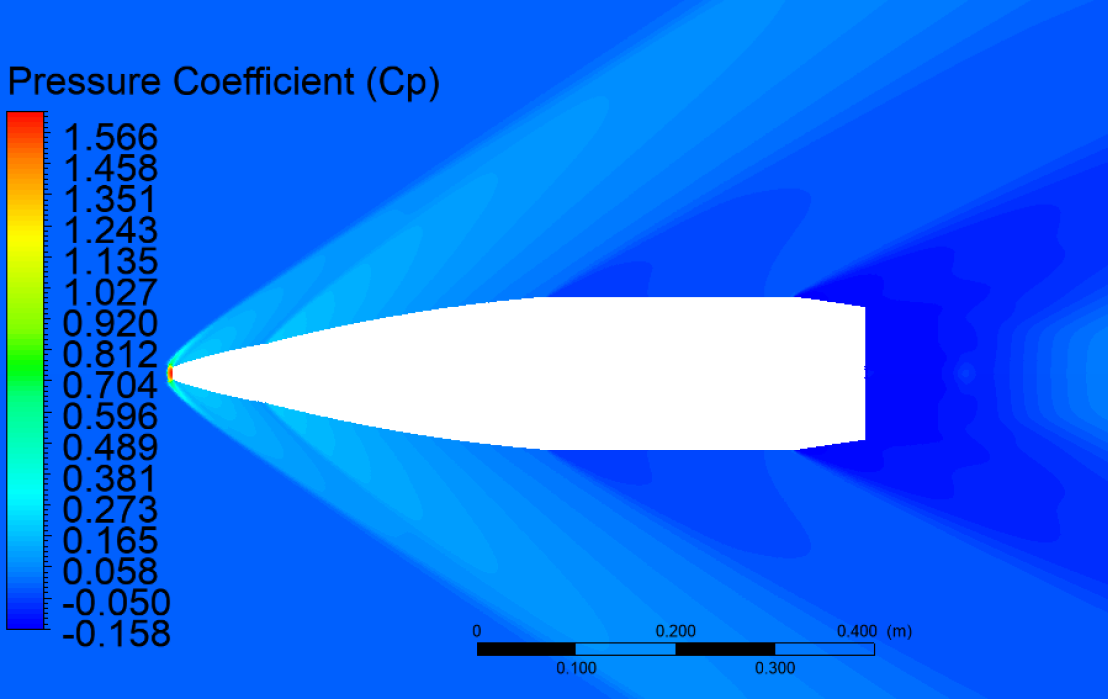
\includegraphics[height=5cm,width=\textwidth]{contorno-pressao-2306K-vazao-0030-1pol.png}
        \caption{Contornos de Pressão - \(\Dot{m}_{BB}\) = \qty{0,030}{\kilogram\per\second}}
        \label{fig:contorno-pressao-bb-1pol-vazao0030}
    \end{subfigure}
    \hfill
    \begin{subfigure}[b]{0.47\textwidth}
        \centering
        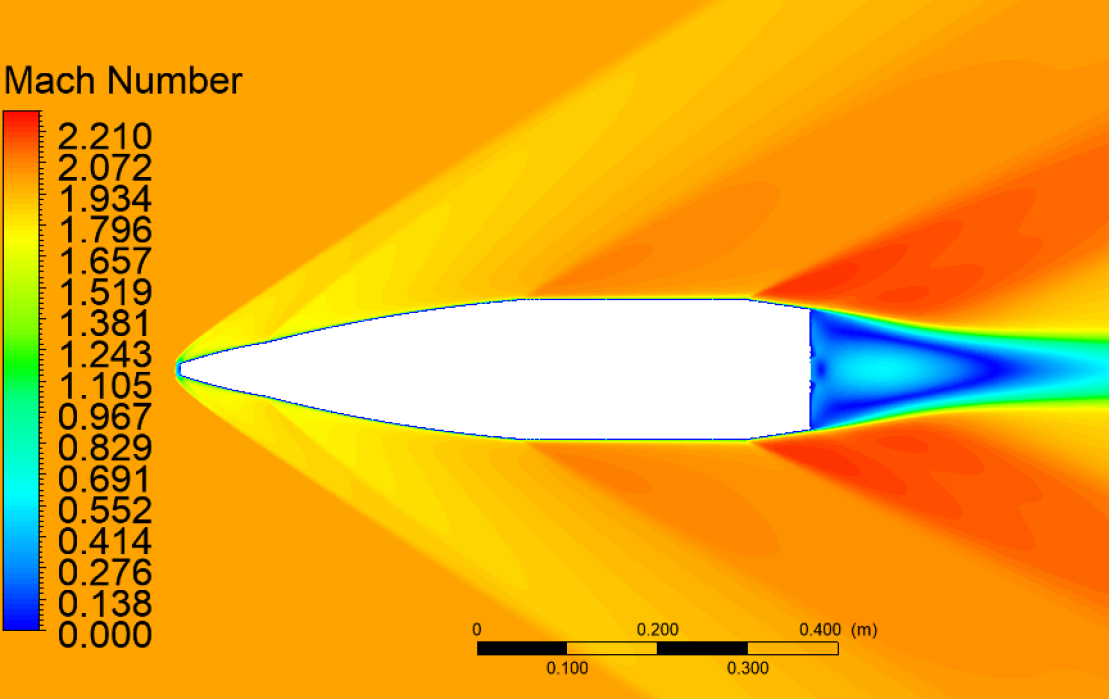
\includegraphics[height=5cm,width=\textwidth]{contorno-velocidade-2306K-vazao-0015-1pol.png}
        \caption{Cont. de Velocidade - \(\Dot{m}_{BB}\) = \qty{0,015}{\kilogram\per\second}}
        \label{fig:contorno-velocidade-bb-1pol-vazao0015}
    \end{subfigure}
    \hfill
	\begin{subfigure}[b]{0.47\textwidth}
        \centering
        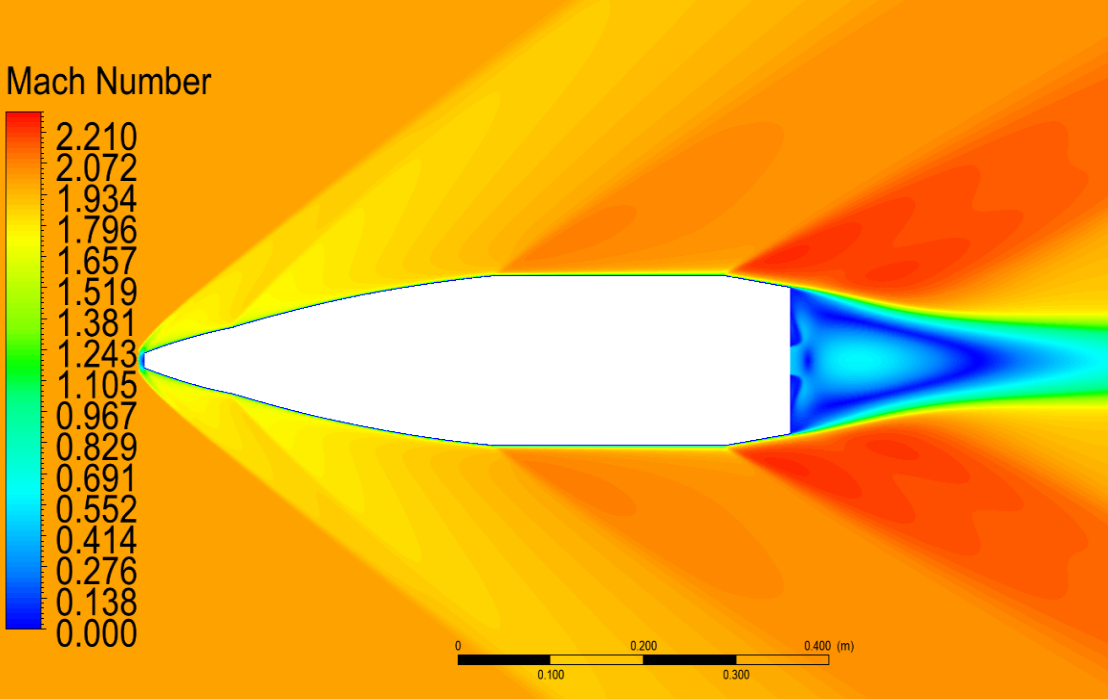
\includegraphics[height=5cm,width=\textwidth]{contorno-velocidade-2306K-vazao-0030-1pol.png}
        \caption{Cont. de Velocidade - \(\Dot{m}_{BB}\) = \qty{0,030}{\kilogram\per\second}}
        \label{fig:contorno-velocidade-bb-1pol-vazao0030}
    \end{subfigure}
    \hfill
    \begin{subfigure}[b]{0.47\textwidth}
        \centering
        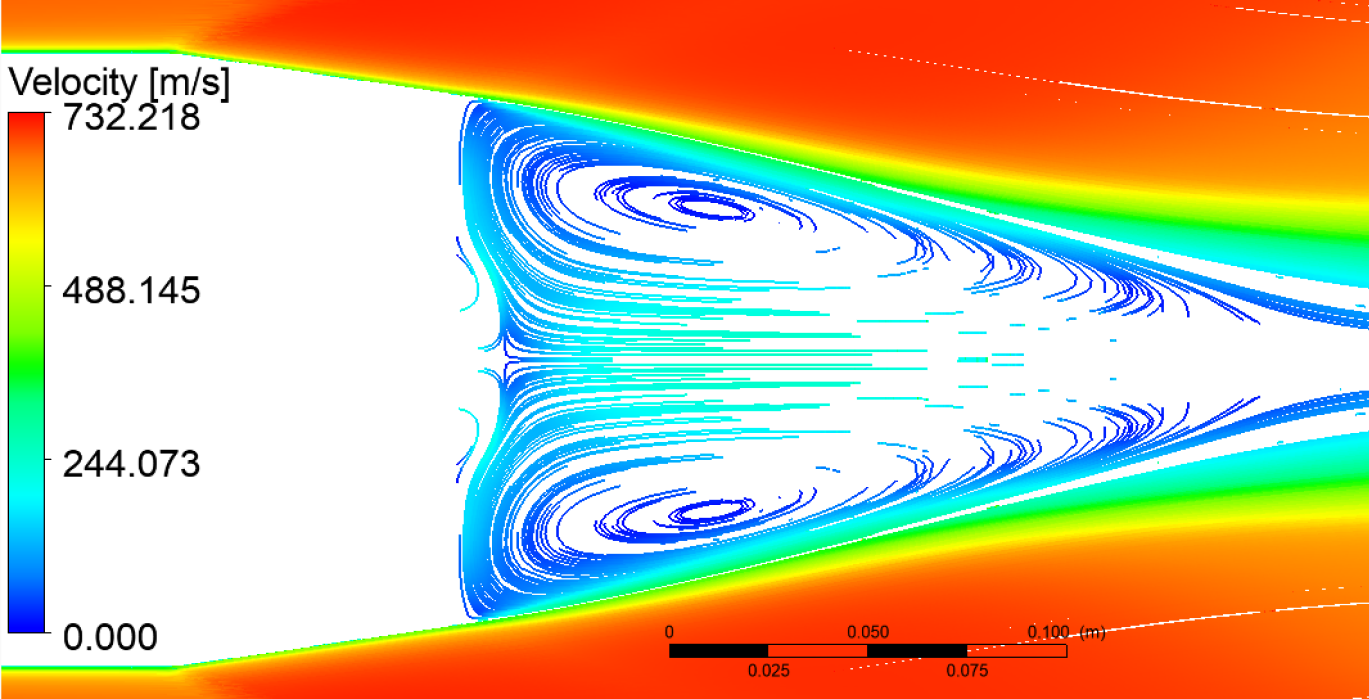
\includegraphics[height=5cm,width=\textwidth]{corrente-velocidade-2306K-vazao-0015-1pol.png}
        \caption{Linhas de corrente - \(\Dot{m}_{BB}\) = \qty{0,015}{\kilogram\per\second}}
        \label{fig:corrente-velocidade-bb-1pol-vazao0015}
    \end{subfigure}
    \hfill
    \begin{subfigure}[b]{0.47\textwidth}
        \centering
        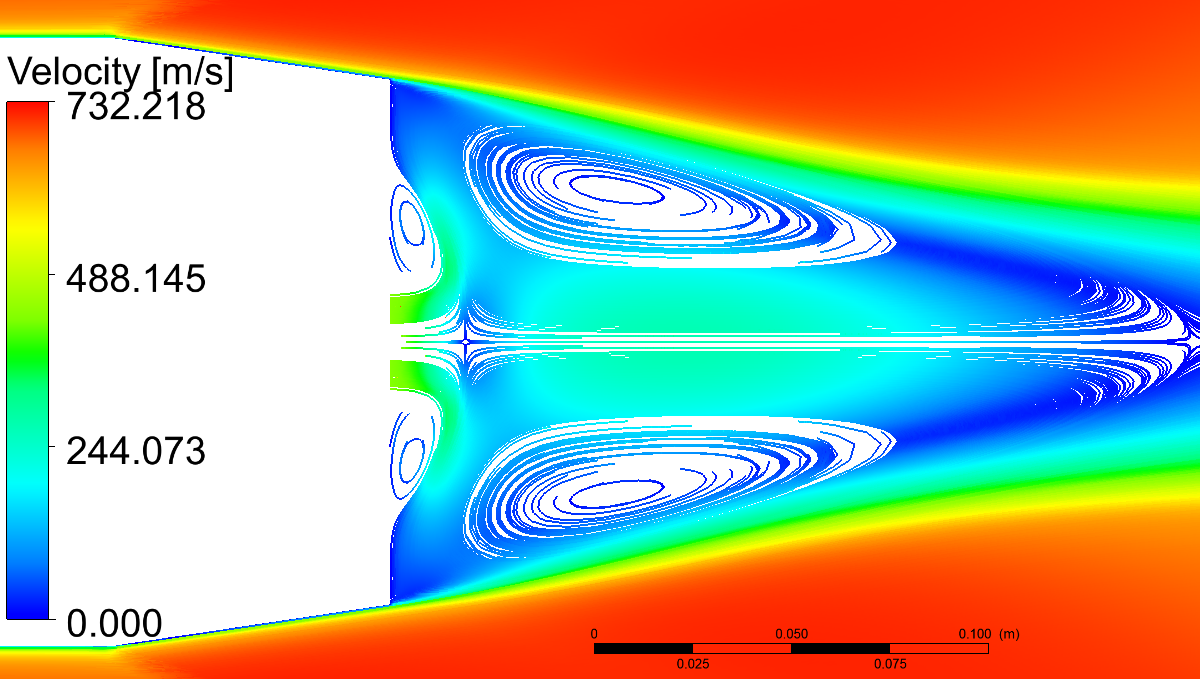
\includegraphics[height=5cm,width=\textwidth]{corrente-velocidade-2306K-vazao-0030-1pol.png}
        \caption{Linhas de corrente - \(\Dot{m}_{BB}\) = \qty{0,030}{\kilogram\per\second}}
        \label{fig:corrente-velocidade-bb-1pol-vazao0030}
    \end{subfigure}
	\caption{Projetil sob diferentes condições de vazão mássica sob regime M = \num{2,0} \(\left(\phi_{BB} = \qty{25,4}{\millimetre}; T_{BB} = \qty{2306,15}{\kelvin}\right)\)}
	\label{fig:influencia-diametro-vazao-1pol}
\end{figure}

O passo seguinte foi apresentar o escoamento no entorno do projetil assumindo que o diâmetro de saída do bocal, \(\phi_{BB}\), seja igual a 50,8 mm. Assim como na \autoref{fig:influencia-diametro-vazao-1pol}, a velocidade do meio livre foi definida como M = \num{2,0} para os contornos de pressão e de velocidade, além das linhas de corrente, sendo todos esses perfis vistos na \autoref{fig:influencia-diametro-vazao-2pol}.

Seja na \autoref{fig:contorno-velocidade-bb-2pol-vazao-0030} ou na \autoref{fig:contorno-velocidade-bb-2pol-vazao-0060}, a formação da recirculação é bastante proeminente, acima de tudo no caso em que a vazão mássica é igual a \(\qty{0,060}{\kilogram\per\second}\). Todavia, não se relata nenhuma variação significativa no campo de pressão, como demonstrado nas Figuras \ref{fig:contorno-pressao-bb-2pol-vazao-0030} e \ref{fig:contorno-pressao-bb-2pol-vazao-0060}. No entanto, é com as Figuras \ref{fig:corrente-velocidade-bb-2pol-vazao-0030} e \ref{fig:corrente-velocidade-bb-2pol-vazao-0060} que se ratifica a influência do diâmetro do bocal. As linhas de corrente observadas na \autoref{fig:corrente-velocidade-bb-2pol-vazao-0060} se aproximam das referências \cite{Sahu1985,Mahmoud2009,Lucena2020}. Por esta razão acredita-se que houve a maior redução do arrasto na escolha do maior diâmetro de saída do sistema BB (\qty{2}{\polegada}).

\begin{figure}[!ht]
	\centering
	\begin{subfigure}[b]{0.47\textwidth}
        \centering
        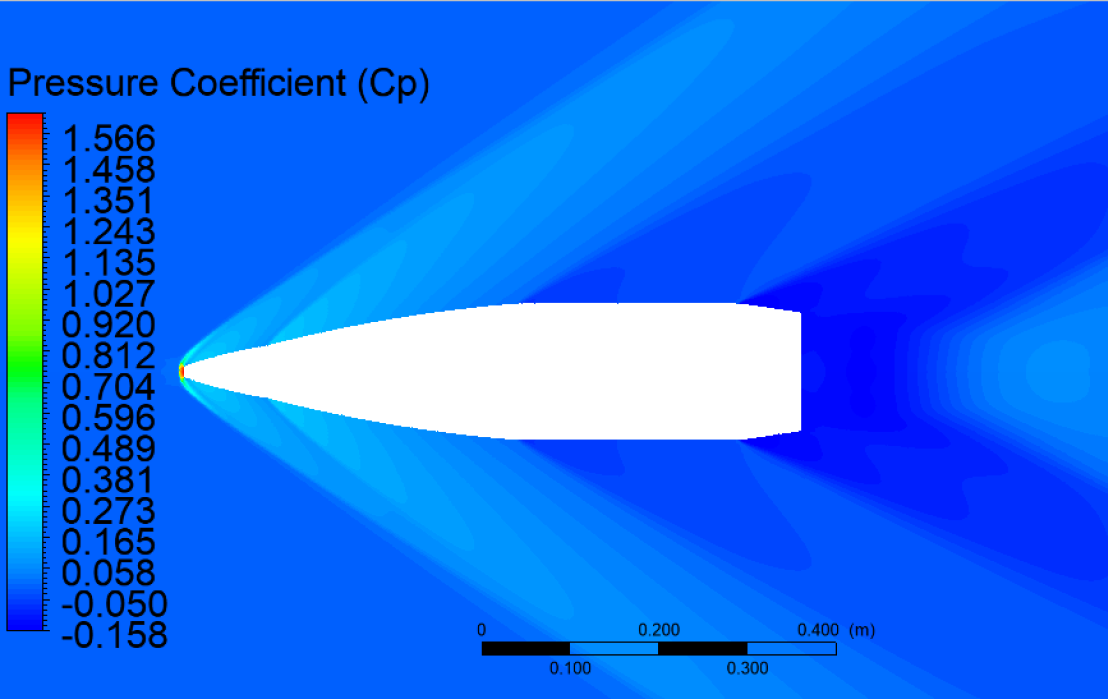
\includegraphics[height=5cm,width=\textwidth]{contorno-pressao-2306K-vazao-0030-2pol.png}
        \caption{Contornos de Pressão - \(\Dot{m}_{BB}\) = \qty{0,030}{\kilogram\per\second}}
        \label{fig:contorno-pressao-bb-2pol-vazao-0030}
    \end{subfigure}
    \hfill
    \begin{subfigure}[b]{0.47\textwidth}
        \centering
        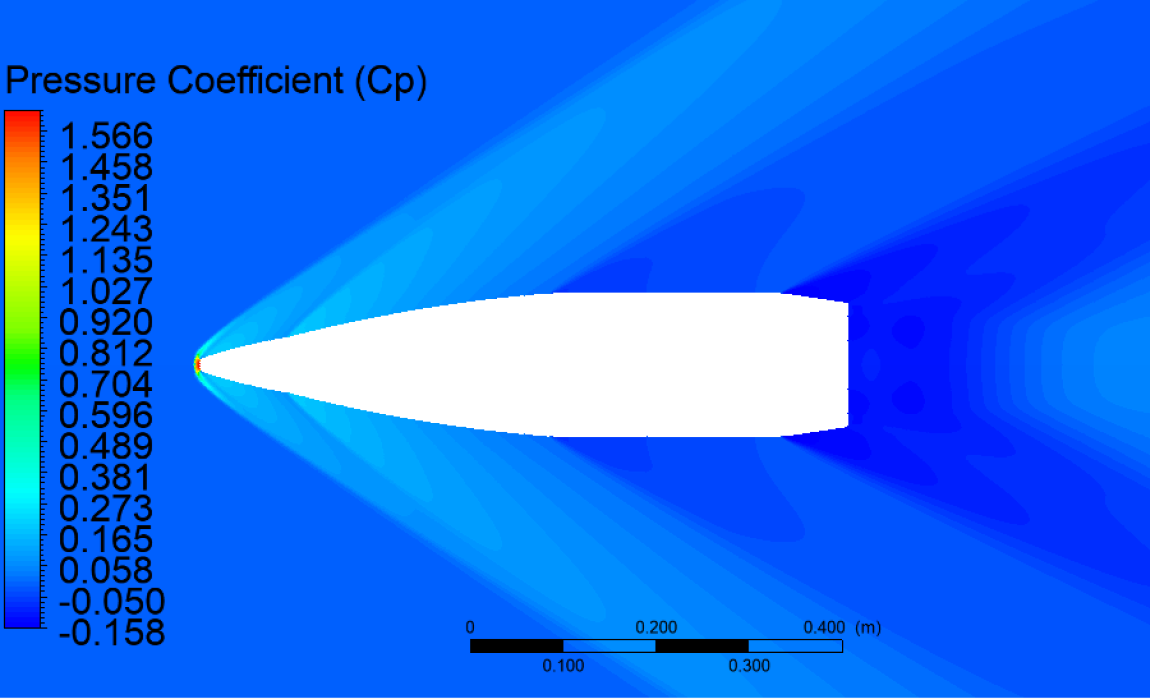
\includegraphics[height=5cm,width=\textwidth]{contorno-pressao-2306K-vazao-0060-2pol.png}
        \caption{Contornos de Pressão - \(\Dot{m}_{BB}\) = \qty{0,060}{\kilogram\per\second}}
        \label{fig:contorno-pressao-bb-2pol-vazao-0060}
    \end{subfigure}
    \hfill
    \begin{subfigure}[b]{0.47\textwidth}
        \centering
        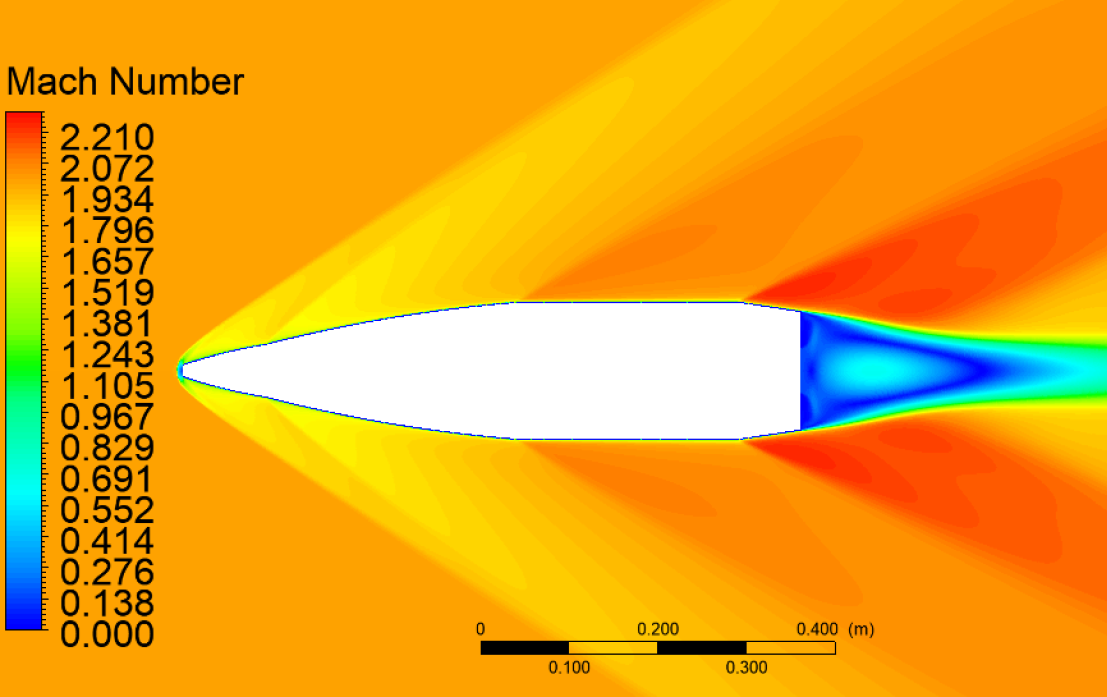
\includegraphics[height=5cm,width=\textwidth]{contorno-velocidade-2306K-vazao-0030-2pol.png}
        \caption{Cont. de Velocidade - \(\Dot{m}_{BB}\) = \qty{0,030}{\kilogram\per\second}}
        \label{fig:contorno-velocidade-bb-2pol-vazao-0030}
    \end{subfigure}
    \hfill
	\begin{subfigure}[b]{0.47\textwidth}
        \centering
        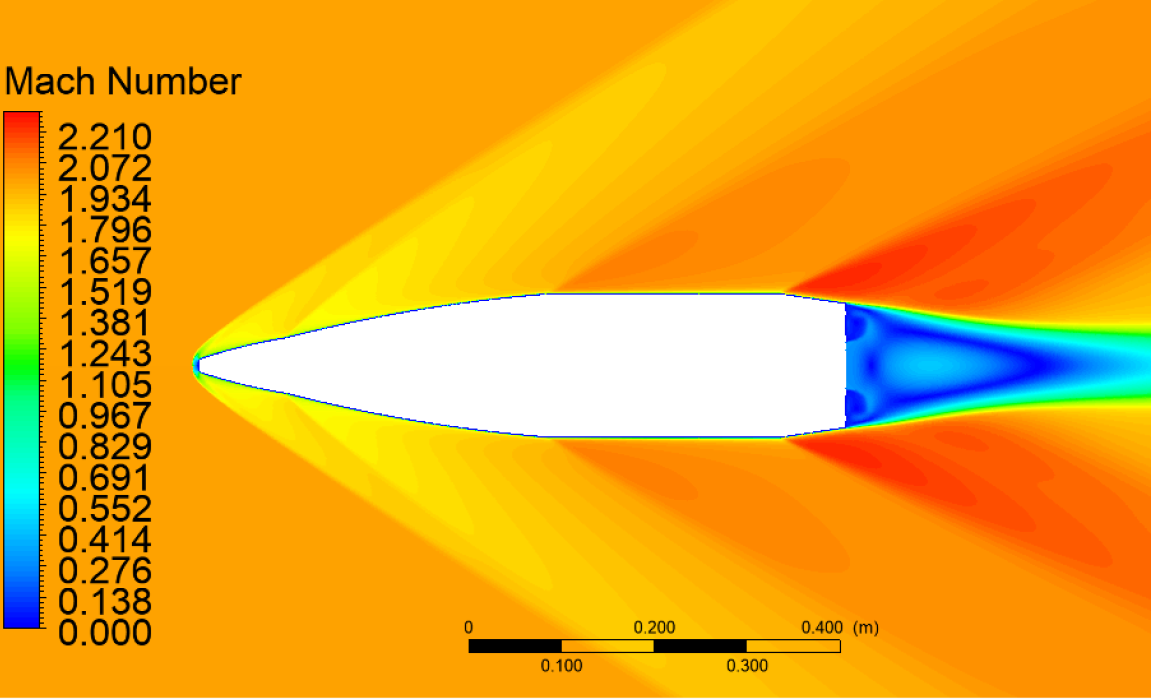
\includegraphics[height=5cm,width=\textwidth]{contorno-velocidade-2306K-vazao-0060-2pol.png}
        \caption{Cont. de Velocidade - \(\Dot{m}_{BB}\) = \qty{0,060}{\kilogram\per\second}}
        \label{fig:contorno-velocidade-bb-2pol-vazao-0060}
    \end{subfigure}
	\hfill
	\begin{subfigure}[b]{0.47\textwidth}
        \centering
        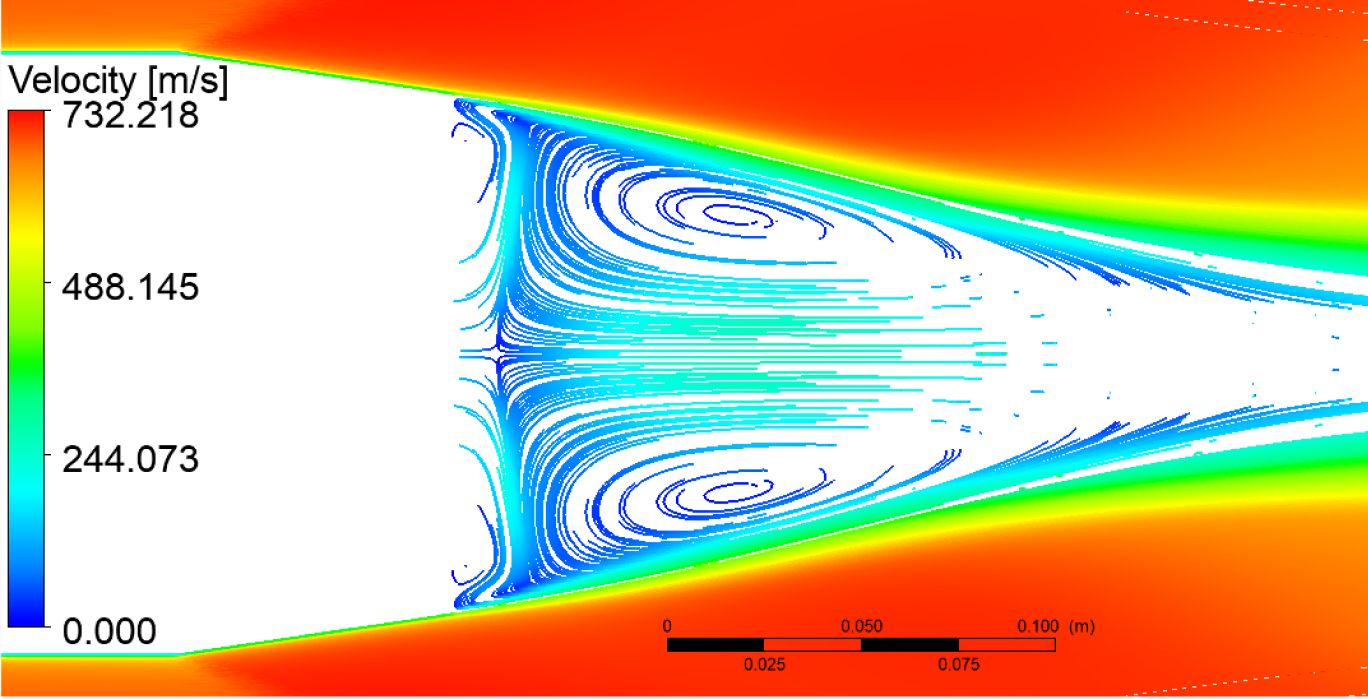
\includegraphics[height=5cm,width=\textwidth]{corrente-velocidade-2306K-vazao-0030-2pol.png}
        \caption{Linhas de Corrente - \(\Dot{m}_{BB}\) = \qty{0,030}{\kilogram\per\second}}
        \label{fig:corrente-velocidade-bb-2pol-vazao-0030}
    \end{subfigure}
    \hfill
    \begin{subfigure}[b]{0.47\textwidth}
        \centering
        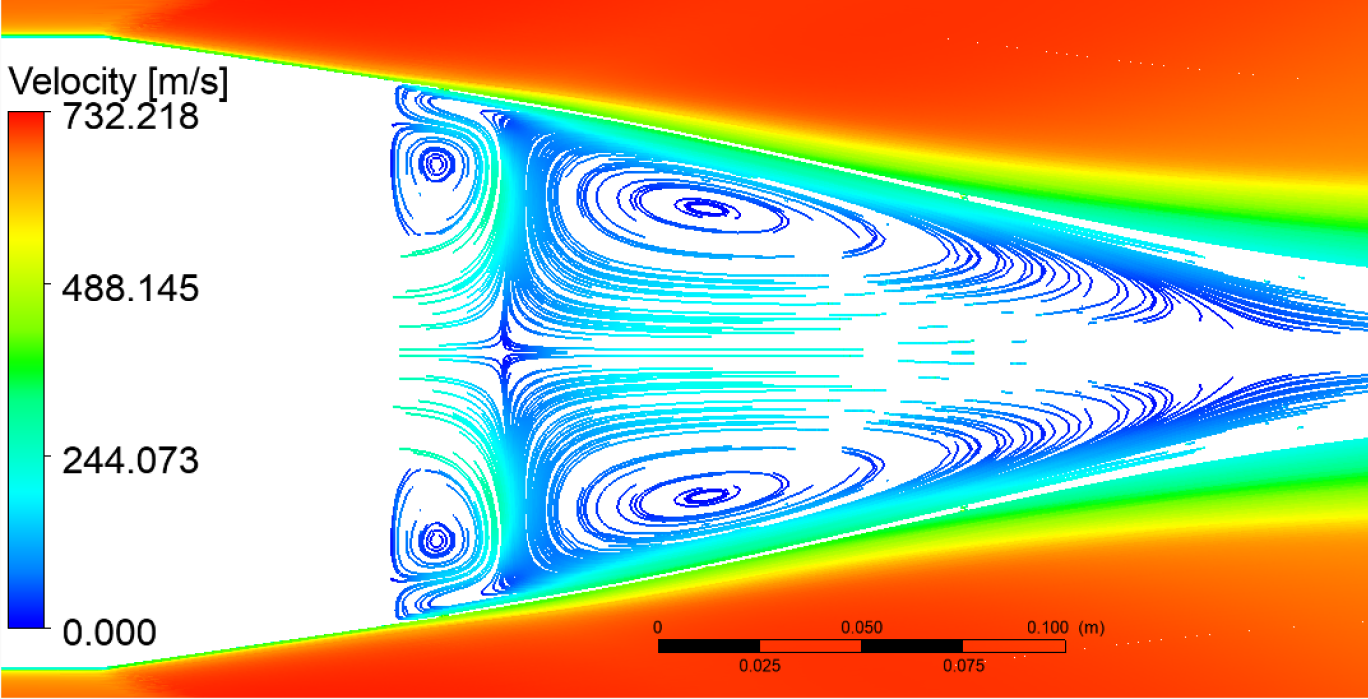
\includegraphics[height=5cm,width=\textwidth]{corrente-velocidade-2306K-vazao-0060-2pol.png}
        \caption{Linhas de Corrente - \(\Dot{m}_{BB}\) = \qty{0,060}{\kilogram\per\second}}
	\label{fig:corrente-velocidade-bb-2pol-vazao-0060}
    \end{subfigure}
	\caption{Projetil sob diferentes condições de vazão mássica sob regime M = \num{2,0} \(\left(\phi_{BB} = \qty{50,8}{\millimetre}; T_{BB} = \qty{2306,15}{\kelvin}\right)\)}
	\label{fig:influencia-diametro-vazao-2pol}
\end{figure}

\subsection{Influência da vazão mássica no sistema \textit{Base Bleed}} \label{subsec:resultados-com-basebleed-vazao}

A \autoref{fig:comparacao-basebleed-vazao} demonstra a influência da vazão nos resultados obtidos nas simulações computacionais com o efeito \textit{Base Bleed} na base do projetil, assumindo que a temperatura de saída dos gases foi fixada em \qty{1500}{\kelvin} e o diâmetro de saída do \textit{Base Bleed} escolhido foi de \qty{2}{\polegada} \(\left(\phi_{BB} = \qty{50,8}{\millimetre}\right)\). A escolha por esse diâmetro de saída se deve aos melhores resultados produzidos na \autoref{subsec:resultados-com-basebleed-diametros}.

Acerca do coeficiente de arrasto, nota-se na \autoref{fig:comparacao-basebleed-vazao} uma redução dos valores conforme aumenta a vazão mássica, \(\Dot{m}_{BB}\). As oscilações nos valores continuam aparecendo no regime subsônico, apesar de seguirem a mesma tendência, não importando qual vazão seja. O regime transônico reúne as maiores reduções do arrasto aerodinâmico, mas a redução do arrasto se faz menos efeito conforme aumenta a velocidade, passando pelo supersônico, especialmente quando M > \num{2,0}.

\begin{figure}[!ht]
	\centering
	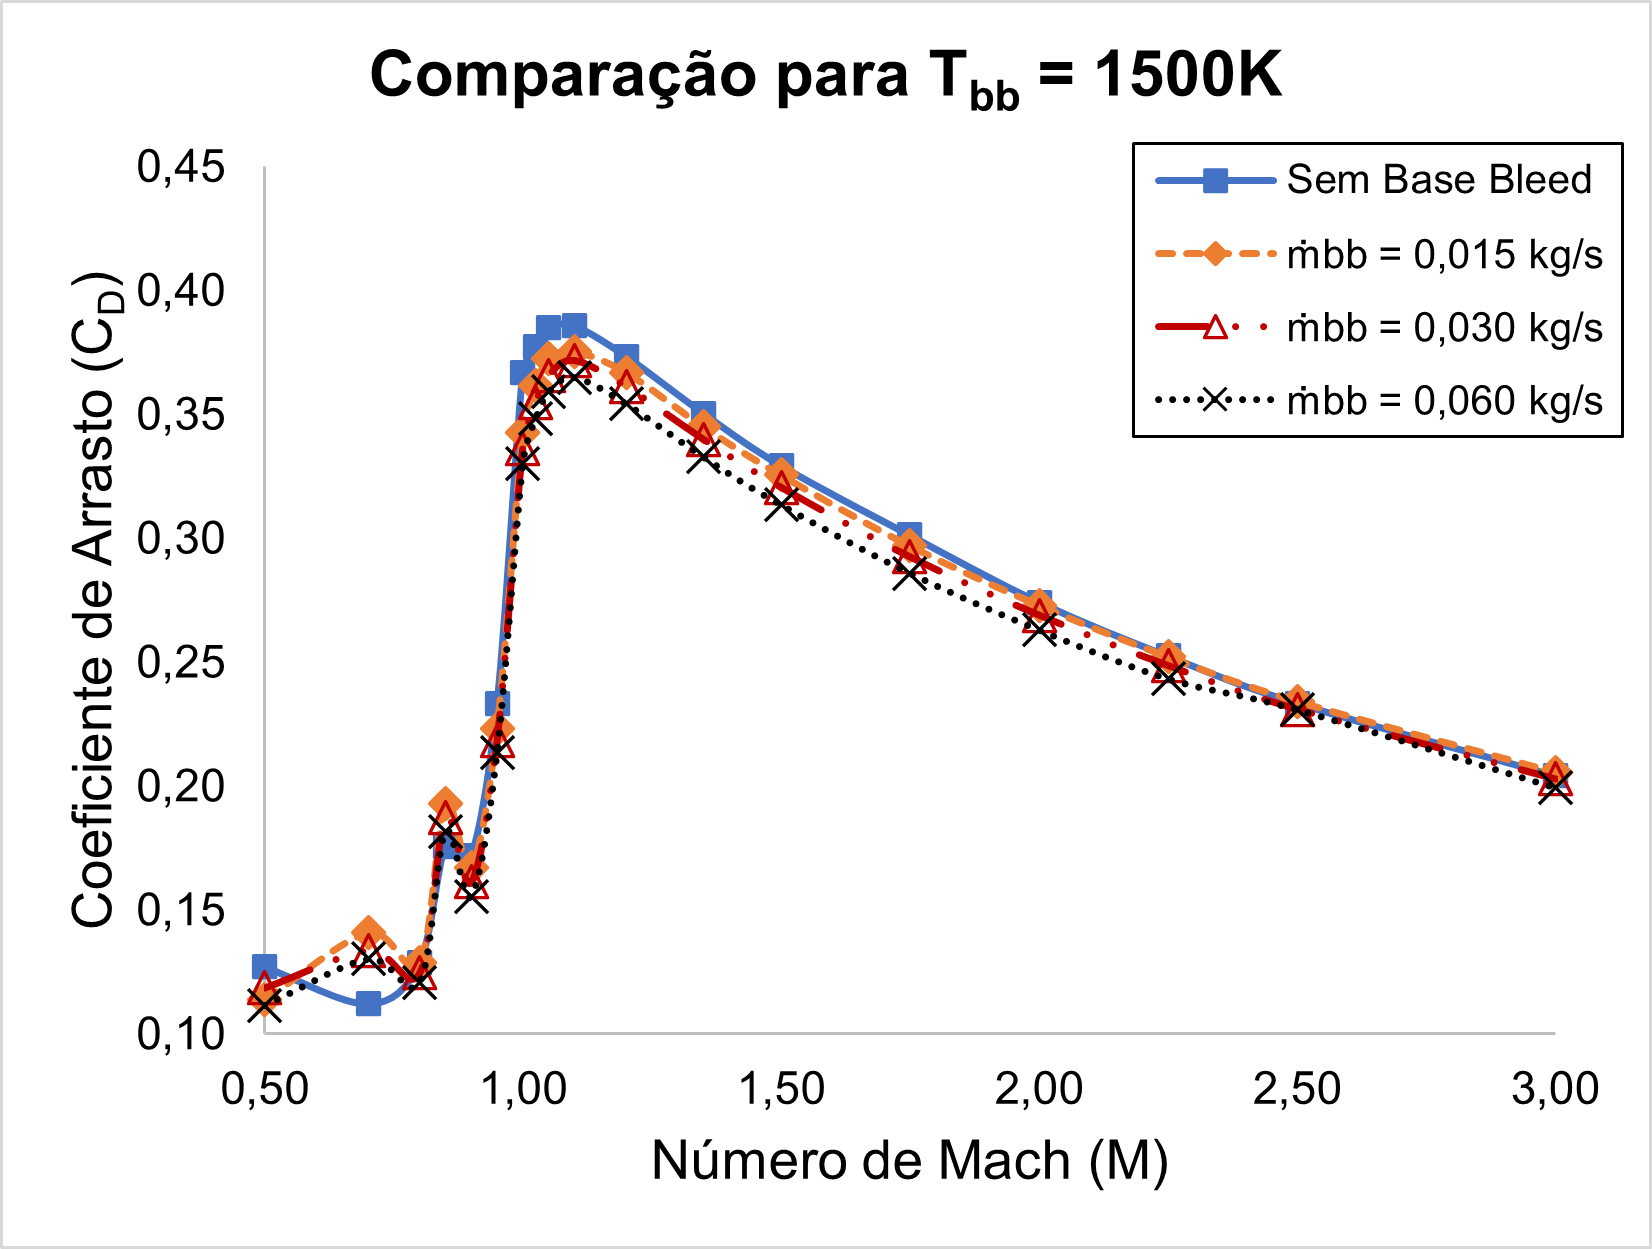
\includegraphics[width=0.5\textwidth]{cd-combasebleed-1500K-2pol.png}
	\caption{Influência da vazão mássica do \textit{Base Bleed} - \(T_{BB}\) = \qty{1500}{\kelvin}}
	\label{fig:comparacao-basebleed-vazao}
\end{figure}

\begin{figure}[!ht]
	\centering
	\begin{subfigure}[b]{0.47\textwidth}
        \centering
        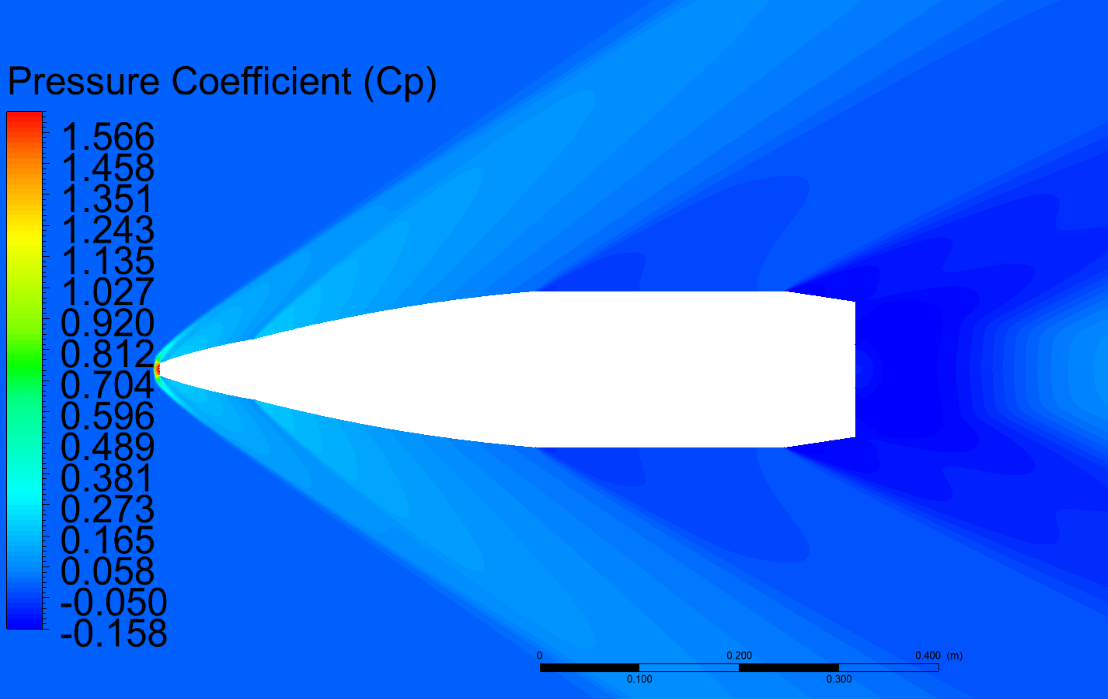
\includegraphics[width=\textwidth,height=5cm]{contorno-pressao-1500K-vazao-0030-2pol.png}
        \caption{Contornos de Pressão - \(\Dot{m}_{BB}\) = \qty{0,060}{\kilogram\per\second}}
        \label{fig:contorno-pressao-bb-1500K-vazao0030}
    \end{subfigure}
    \hfill
    \begin{subfigure}[b]{0.47\textwidth}
        \centering
        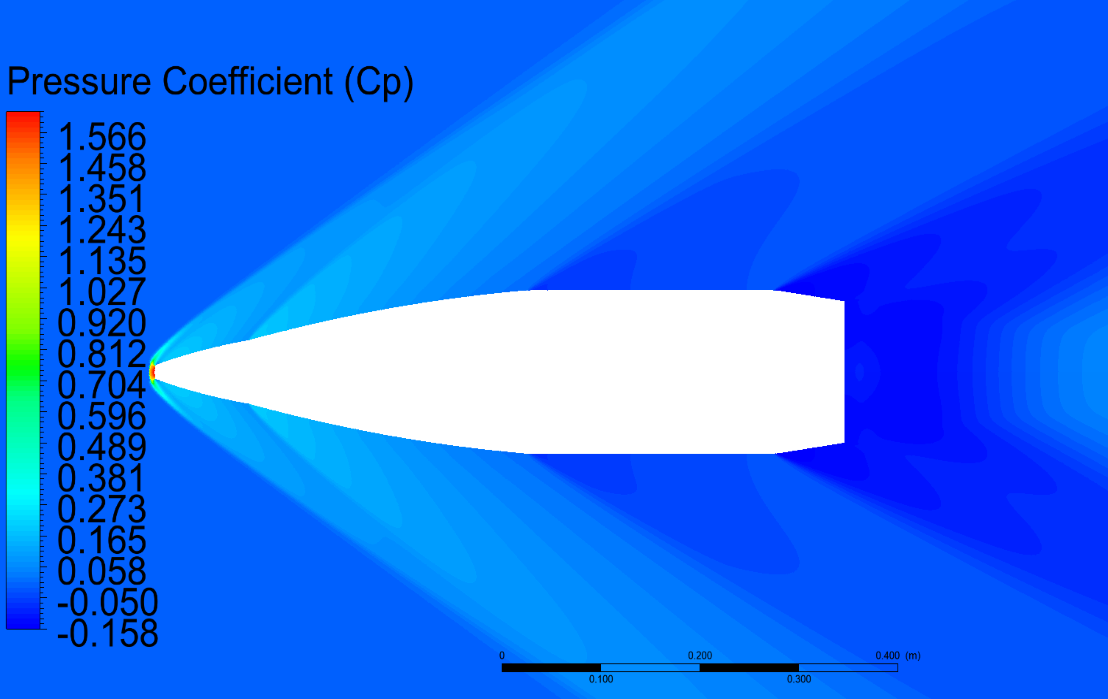
\includegraphics[width=\textwidth,height=5cm]{contorno-pressao-1500K-vazao-0060-2pol.png}
        \caption{Contornos de Pressão - \(\Dot{m}_{BB}\) = \qty{0,060}{\kilogram\per\second}}
        \label{fig:contorno-pressao-bb-1500K-vazao0060}
    \end{subfigure}
    \hfill
	\begin{subfigure}[b]{0.47\textwidth}
        \centering
        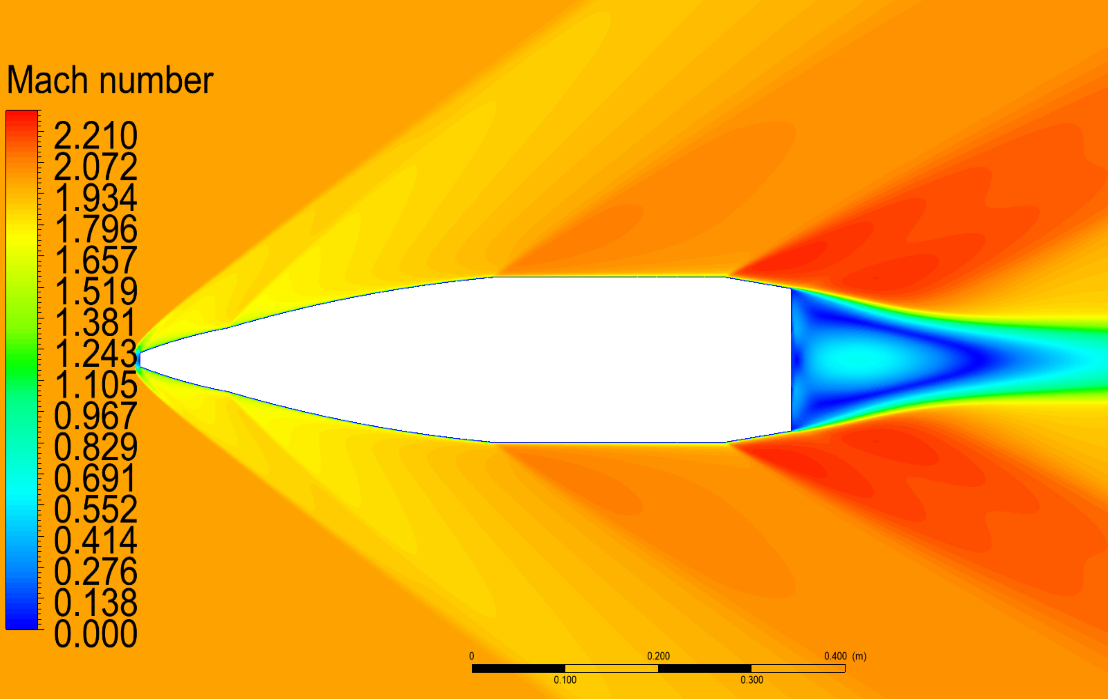
\includegraphics[width=\textwidth,height=5cm]{contorno-velocidade-1500K-vazao-0030-2pol.png}
        \caption{Cont. de Velocidade - \(\Dot{m}_{BB}\) = \qty{0,060}{\kilogram\per\second}}
        \label{fig:contorno-velocidade-bb-1500K-vazao0030}
    \end{subfigure}
    \hfill
	\begin{subfigure}[b]{0.47\textwidth}
        \centering
        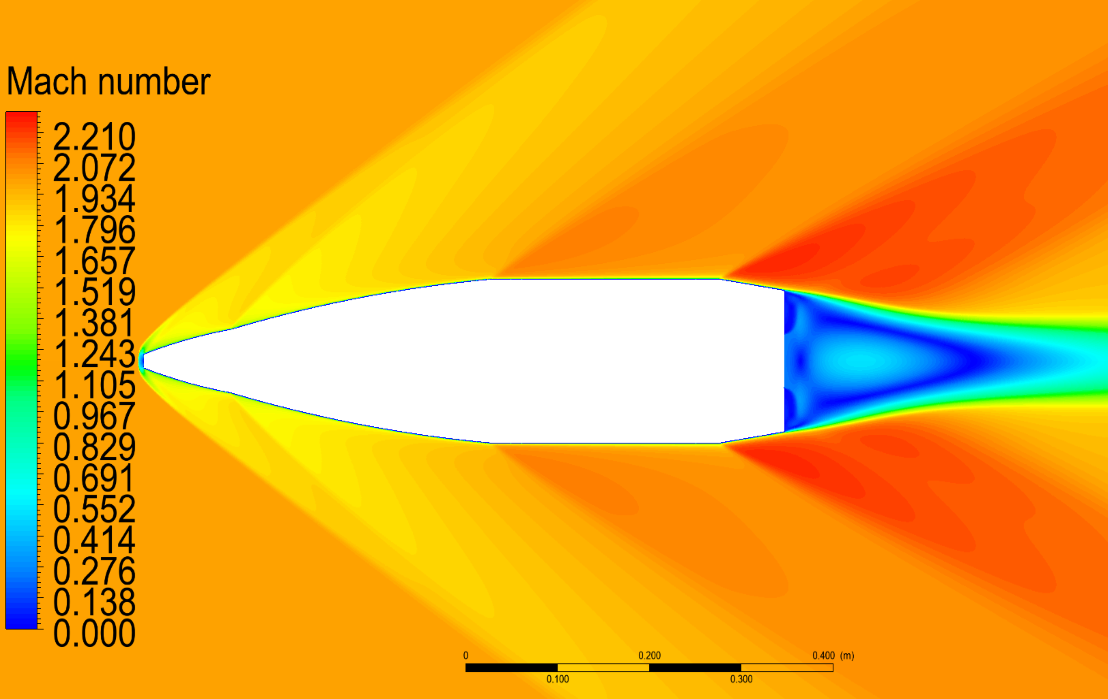
\includegraphics[width=\textwidth,height=5cm]{contorno-velocidade-1500K-vazao-0060-2pol.png}
        \caption{Cont. de Velocidade - \(\Dot{m}_{BB}\) = \qty{0,060}{\kilogram\per\second}}
        \label{fig:contorno-velocidade-bb-1500K-vazao0060}
    \end{subfigure}
    \begin{subfigure}[b]{0.47\textwidth}
        \centering
        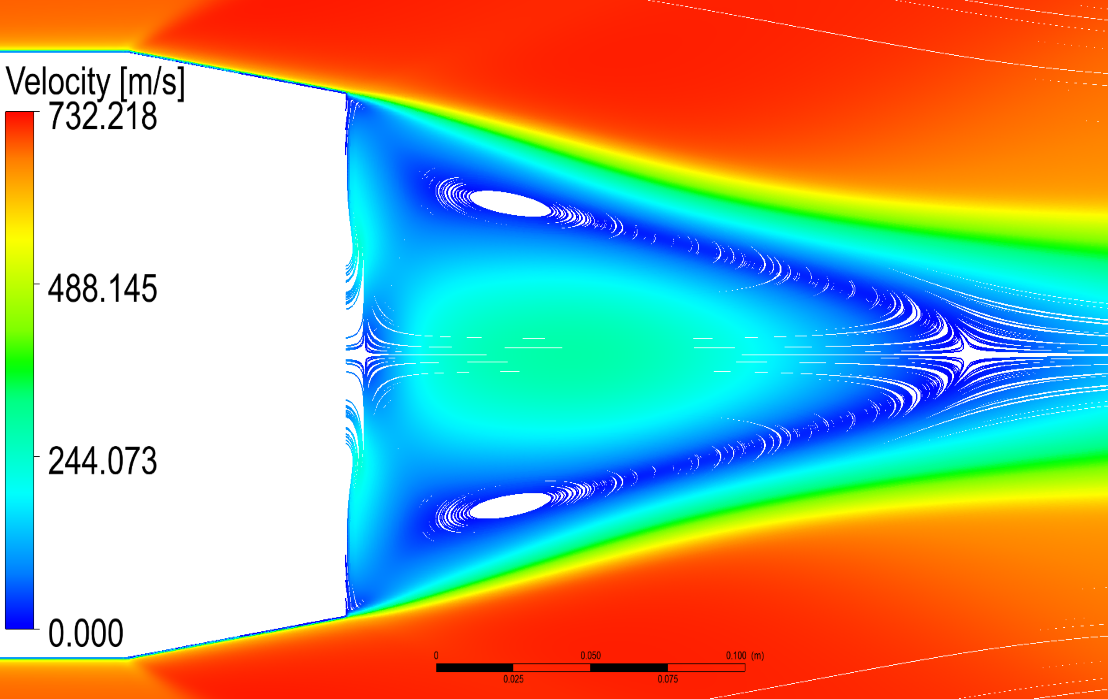
\includegraphics[width=\textwidth,height=5cm]{corrente-velocidade-1500K-vazao-0030-2pol.png}
        \caption{Linhas de Corrente - \(\Dot{m}_{BB}\) = \qty{0,060}{\kilogram\per\second}}
        \label{fig:corrente-velocidade-bb-1500K-vazao0030}
    \end{subfigure}
    \hfill
	\begin{subfigure}[b]{0.47\textwidth}
        \centering
        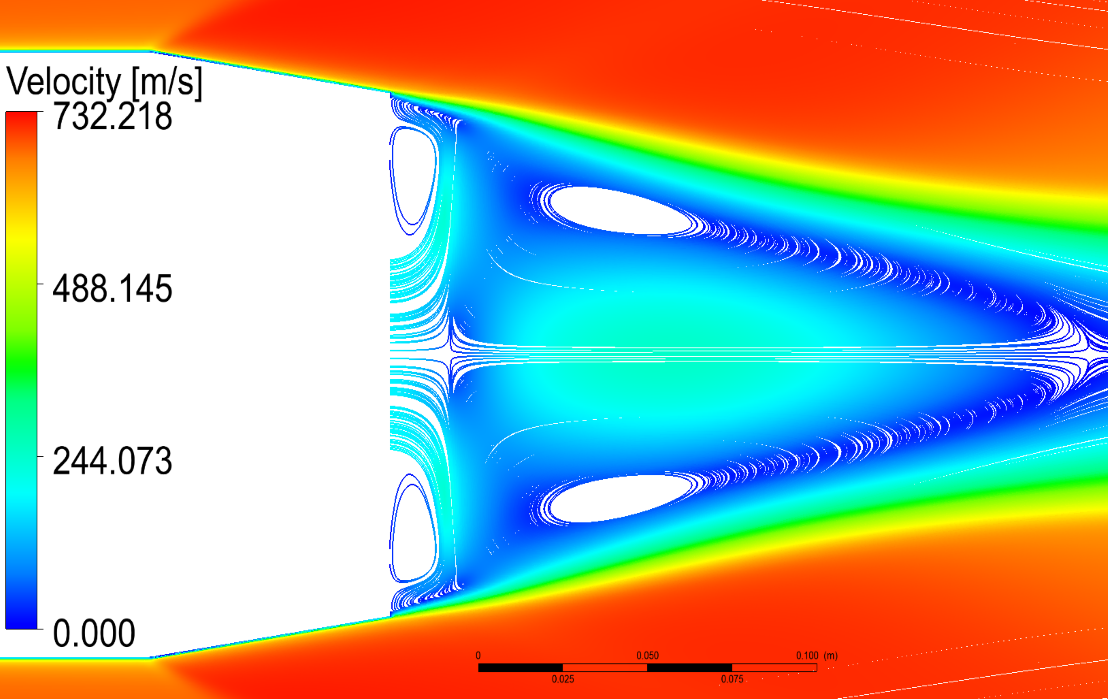
\includegraphics[width=\textwidth,height=5cm]{corrente-velocidade-1500K-vazao-0060-2pol.png}
        \caption{Linhas de Corrente - \(\Dot{m}_{BB}\) = \qty{0,060}{\kilogram\per\second}}
        \label{fig:corrente-velocidade-bb-1500K-vazao0060}
    \end{subfigure}
    \caption{Projetil sob diferentes condições de vazão mássica sob regime M = \num{2,0} \(\left(\phi_{BB} = \qty{50,8}{\millimetre}; T_{BB} = \qty{1500}{\kelvin}\right)\)}
	\label{fig:influencia-temperatura-bb}
\end{figure}

Conforme aumenta a vazão, há um aumento de velocidade, apesar de não haver acréscimo de pressão, o que é demonstrado pela \autoref{fig:contorno-pressao-bb-1500K-vazao0030} ou \autoref{fig:contorno-pressao-bb-1500K-vazao0060}. Os contornos de velocidade, presentes nas Figuras \ref{fig:contorno-velocidade-bb-1500K-vazao0030} e \ref{fig:contorno-velocidade-bb-1500K-vazao0060}, apresentam o deslocamento da região primária de recirculação, além do aumento da esteira turbulenta. 

Pelas Figuras \ref{fig:corrente-velocidade-bb-1500K-vazao0030} e \ref{fig:corrente-velocidade-bb-1500K-vazao0060} se observam as linhas de corrente para a velocidade. Em ambos os casos há a formação da recirculação anular, mas essa zona secundária de recirculação é mais proeminente conforme o aumento da vazão. A \autoref{fig:corrente-velocidade-bb-1500K-vazao0060} apresenta com maior clareza um valor mais próximo do que se espera ocorrer na região, dentro do que a literatura demonstrou em trabalhos anteriores \cite{Sahu1985,Andersson1976}. Assume-se que todos os contornos da \autoref{fig:influencia-temperatura-bb} estão sob regime M = \num{2,0}.

\subsection{Influência da temperatura}

A \autoref{fig:comparacao-basebleed-temperatura} demonstra a influência da temperatura nos resultados obtidos nas simulações computacionais com o efeito \textit{Base Bleed} na base do projetil, assumindo que a vazão mássica de saída dos gases foi fixada em \qty{0,060}{\kilogram\per\second} e o diâmetro de saída do \textit{Base Bleed} escolhido foi de \qty{2}{\polegada} \(\left(\phi_{BB} = \qty{50,8}{\millimetre}\right)\). A escolha por esse diâmetro de saída se deve aos melhores resultados produzidos na \autoref{subsec:resultados-com-basebleed-diametros}. A escolha pela vazão de \qty{0,060}{\kilogram\per\second} se baseou nos resultados das \autoref{subsec:resultados-com-basebleed-vazao}, em que a redução do coeficiente de arrasto foi mais significativo quando comparado ao projetil inerte.

\begin{figure}[!ht]
	\centering
	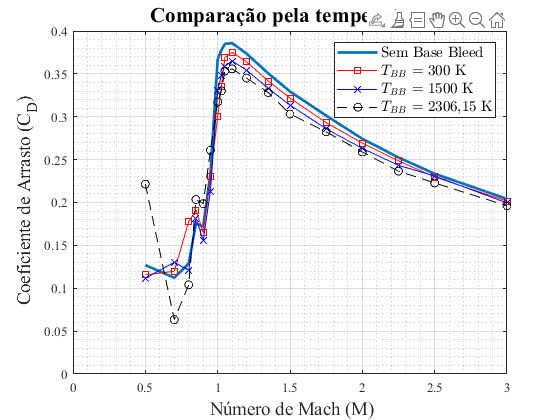
\includegraphics[width=0.5\textwidth]{cd-combasebleed-vazao006-2pol.png}
	\caption{Influência da temperatura do \textit{Base Bleed} sobre o coeficiente de arrasto com \(\Dot{m}_{BB}\) = \qty{0,060}{\kilogram\per\second}}
	\label{fig:comparacao-basebleed-temperatura}
\end{figure}

Acerca do coeficiente de arrasto, nota-se na \autoref{fig:comparacao-basebleed-temperatura} uma redução dos valores conforme aumenta a temperatura, \(Dot{m}_{BB}\). As oscilações nos valores continuam aparecendo no regime subsônico, embora tenham valores discrepantes no início da curva no caso em que a temperatura é mais elevada \(T_{BB} = \qty{2306,15}{\kelvin}\). Mesmo assim, seguem a mesma tendência, não importando qual vazão seja. O regime transônico reúne as maiores reduções do arrasto aerodinâmico, mas a redução do arrasto também é considerável no regime supersônico, principalmente o valor de Mach entre \numrange{1,5}{2,0}. Após esse intervalo, a redução é mais gradual.

\subsection{Influência da abordagem RANS}\label{subsec:resultados-com-basebleed-RANS}

Conforme foi citado anteriormente, o modelo Spalart-Allmaras \cite{Spalart1992} foi manejado para atestar a eficiência de outra técnica RANS para descrição da turbulência além do que foi proposto por \citeauthor{Menter1994TwoequationET}. A comparação foi realizada somente para os seguintes valores na condição de contorno \textit{base bleed inlet}: \(\Dot{m}_{BB}\) = \qty{50,8}{\millimetre}, \(T_{BB} = \qty{2306,15}{\kelvin}\) e \(\Dot{m}_{BB}\) = \qty{0,060}{\kilogram\per\second}.

Entretanto, é notório que o modelo Spalart-Allmaras (S-A) superestimou a curva de arrasto em todos os regimes de velocidade, relatado pela Figura \ref{fig:comparacao-bb-rans}.

\begin{figure}[!ht]
    \centering
    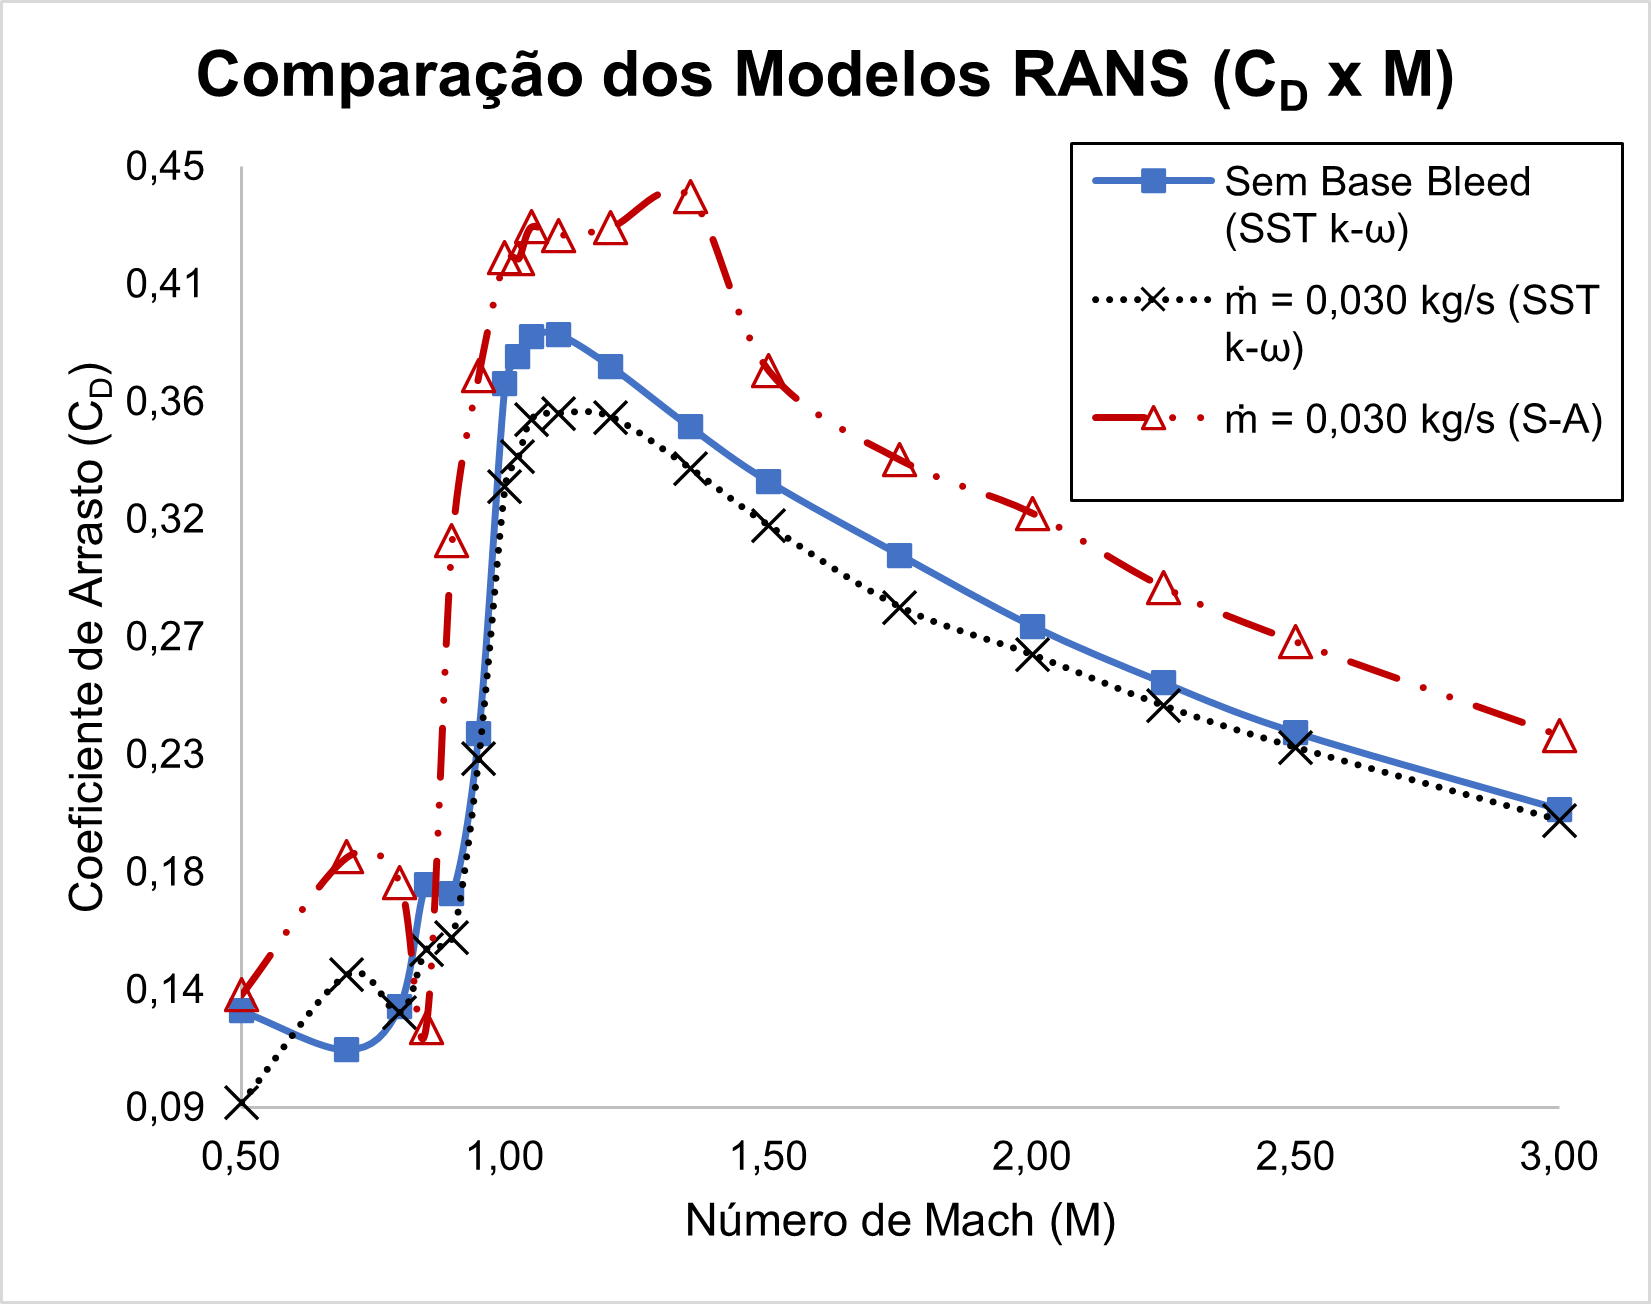
\includegraphics[width=0.5\textwidth]{cd-combasebleed-rans.png}
 	\caption{Curvas de arrasto de acordo com modelos de turbulência RANS}
    \label{fig:comparacao-bb-rans}
\end{figure}

De acordo com a apresentação da \autoref{fig:contornos-pressao-velocidade-RANS}, o modelo S-A não conseguiu encontrar a zona de recirculação gerada pelo sistema \textit{base bleed} como tampouco registra o momento provocado pela vazão mássica de gases do propelente.

\begin{figure}[!ht]
	\centering
	\begin{subfigure}[b]{0.47\textwidth}
        \centering
        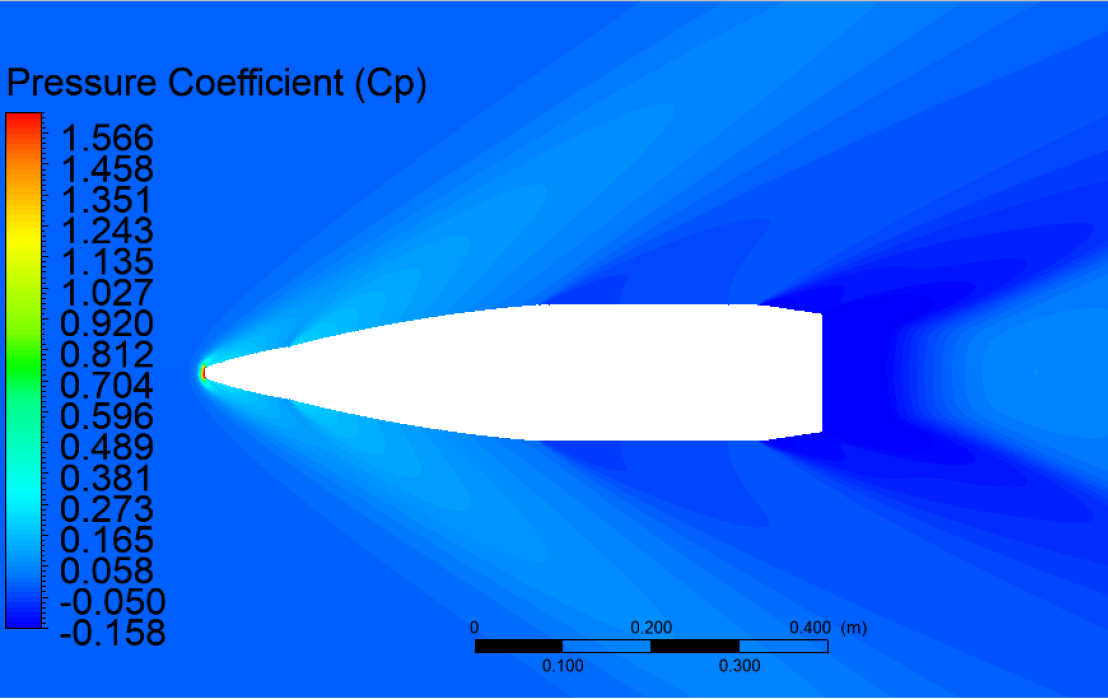
\includegraphics[height=5cm,width=\textwidth]{contorno-pressao-SPALART-2pol.png}
        \caption{Contornos de Pressão}
        \label{fig:contorno-pressao-bb-2pol-RANS}
    \end{subfigure}
    \hfill
    \begin{subfigure}[b]{0.47\textwidth}
        \centering
        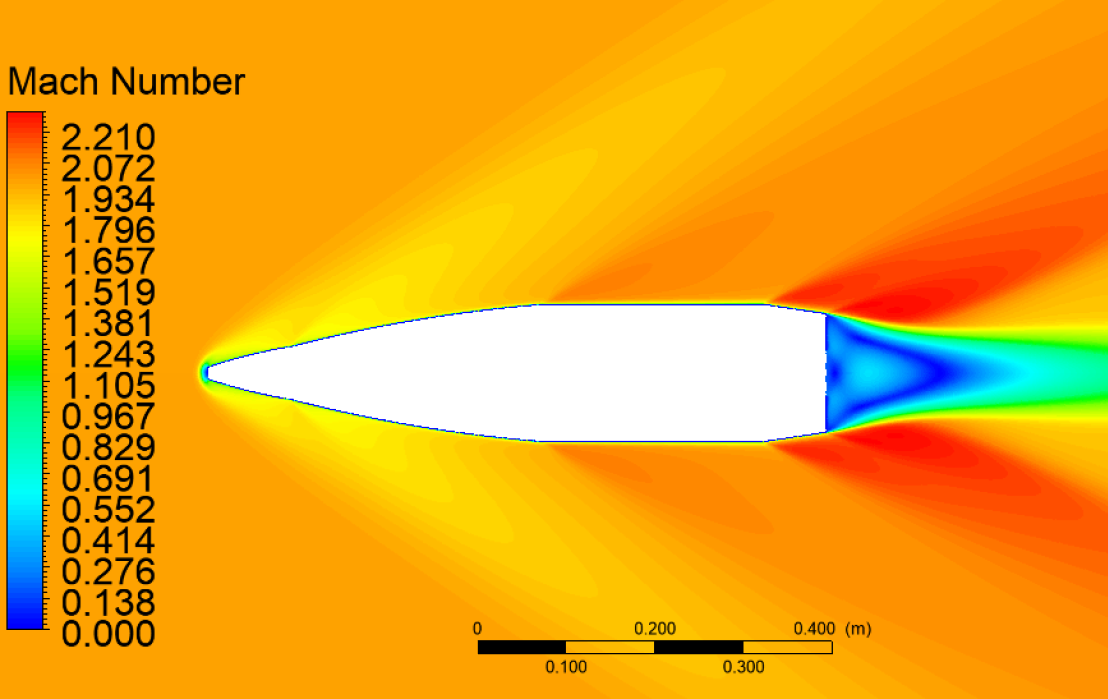
\includegraphics[height=5cm,width=\textwidth]{contorno-velocidade-SPALART-2pol.png}
        \caption{Contornos de Velocidade}
        \label{fig:contorno-velocidade-bb-2pol-RANS}
    \end{subfigure}
	\caption{Projetil sob modelo Spalart-Allmaras}
	\label{fig:contornos-pressao-velocidade-RANS}
\end{figure}

Para assegurar o que foi demonstrado na \autoref{fig:contorno-pressao-bb-2pol-RANS}, a \autoref{fig:corrente-velocidade-bb-RANS} foi elaborada para analisar as linhas de corrente com o modelo de 1 equação, donde se concluiu que o alto gradiente adverso de pressão existente no sistema BB resultou em desvios que fogem da explicação do fenômeno físico real, ainda que as técnicas RANS enxerguem os valores médios das propriedades do fluido.

\begin{figure}[!ht]
    \centering
    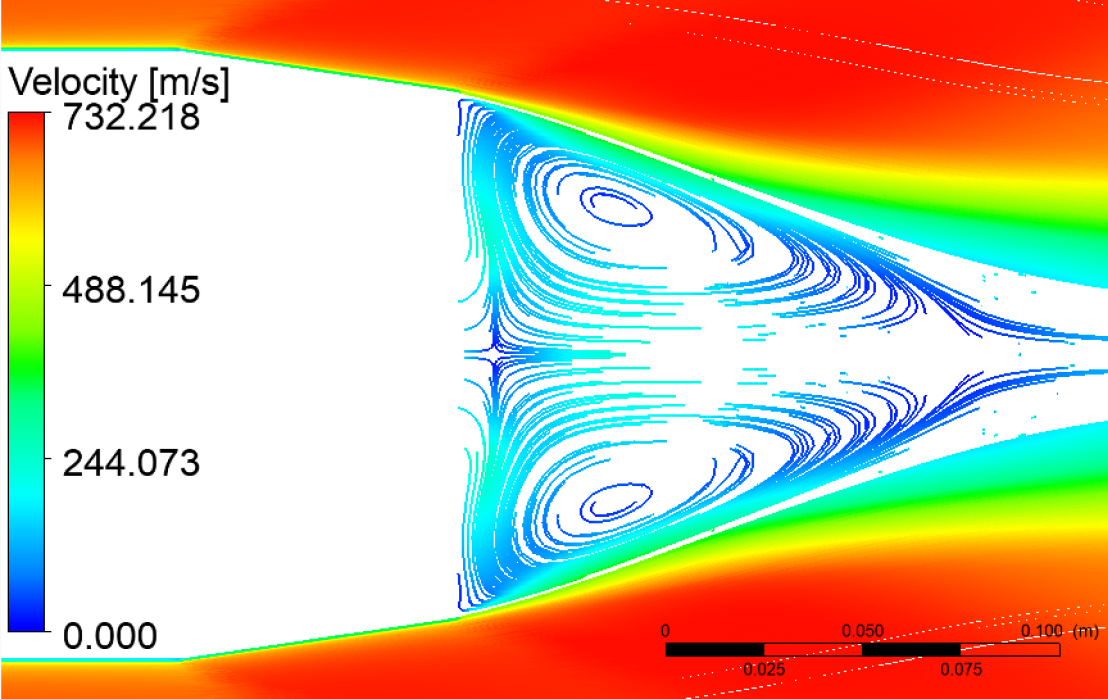
\includegraphics[height=5cm,width=0.5\textwidth]{corrente-velocidade-SPALART-2pol.png}
 	\caption{Linhas de corrente para o modelo Spalart-Allmaras}
    \label{fig:corrente-velocidade-bb-RANS}
\end{figure}

\section{Resultados da Trajetória}\label{sec:resultados-trajetoria}

A partir do momento em que há disponibilidade das condições citadas na \autoref{subsec:implementacao-trajetoria} e dos resultados das simulações de fluidodinâmica computacional, pode-se calcular a predição da trajetória MPMTM. Apesar do suporte do PRODAS® e das informações obtidas, algumas premissas foram consideradas:

\begin{itemize}
    \item Lançamento do Rio de Janeiro, logo a latitude é de \ang{23};
    \item Desprezando efeitos da umidade sobre a atmosfera;
    \item Sem velocidade do vento, assim como citado por \citeauthor{Rosendo2020};
    \item Vazão mássica do propelente é constante durante o acionamento do BB;
    \item Parâmetro ótimo de injeção \(\left(Inj_{0}\right)\) igual a \num{5e-3}, tal como descrito por \citeauthor{DAVENAS1993329};
    \item Assumir que os coeficientes aerodinâmicos são linearmente dependentes do ângulo \(\alpha_{e}\)
\end{itemize}

Pela última condição assumida, logo \(C_{L\alpha^{3}}\) e \(C_{m\alpha^{3}}\) não interferem significativamente as equações \ref{eq:liftMPM} e \ref{eq:guinada-de-reposicao}. Embora a ignição seja um tópico relevante no desempenho, a dificuldade em modelar adequadamente à realidade tornou o assunto um caso a ser tratado em estudos posteriores.
De acordo com o STANAG 4355 \cite{stanag4355}, é necessário obter os fatores \(f_{L}\) e \(i_{BB}\) tais que se adequem à cada simulação realizada. 

Para averiguar a qualidade do código desenvolvido em MATLAB®, os resultados obtidos de acordo com as condições de um projetil \qty{155}{\millimetre} a velocidade de disparo v = \qty{207,3}{\metre\per\second} foram analisadas tanto em função do PRODAS® quanto para uma tabela de tiro. Como pode ser visto na \autoref{tab:tabela-validacao-PRODAS-e-tabela-de-tiro-M107} \cite{Thallyo2022}, os erros foram superiores a \qty{1}{\percent} somente para trajetórias de grandes elevações, em que a literatura prevê inconsistências \cite{McCoy2012,Carlucci2018}.

\begin{table}[ht]
    \centering
    \caption[Resultados obtidos durante a validação (munição \qty{155}{\millimetre} M107)]{Resultados obtidos durante a validação (munição \qty{155}{\millimetre} M107)}
    \vspace{0.5cm}
    \resizebox{\textwidth}{!}{%
    \begin{tabular}{c|c|c|c|c|c|c|c}
    \hline
    \multicolumn{4}{c|}{PRODAS®} &
      \multicolumn{4}{c}{Tabela de tiro} \\ \hline
    \multicolumn{1}{c|}{\multirow{2}{*}{\begin{tabular}[c]{@{}c@{}}Elevação \\ (\unit{\milliradian})\end{tabular}}} &
      \multicolumn{2}{c|}{Alcance (\unit{\metre})} &
      \multirow{2}{*}{\begin{tabular}[c]{@{}c@{}}Erro \\ (\unit{\percent})\end{tabular}} &
      \multicolumn{1}{c|}{\multirow{2}{*}{\begin{tabular}[c]{@{}c@{}}Elevação \\ (\unit{\milliradian})\end{tabular}}} &
      \multicolumn{2}{c|}{Alcance (\unit{\metre})} &
      \multirow{2}{*}{\begin{tabular}[c]{@{}c@{}}Erro \\ (\unit{\percent})\end{tabular}} \\ \cline{2-3} \cline{6-7}
    \multicolumn{1}{c|}{} &
      \multicolumn{1}{c|}{Esperado} &
      \multicolumn{1}{c|}{Obtido} &
       &
      \multicolumn{1}{c|}{} &
      \multicolumn{1}{c|}{Esperado} &
      \multicolumn{1}{c|}{Obtido} &
       \\ \hline
    \num{58,9} &
      \num{500,0} &
      \num{501,2} &
      \num{0,24} &
      \num{58,9} &
      \num{500,0} &
      \num{501,2} &
      \num{0,24} \\
    \num{120,1} &
      \num{1000,0} &
      \num{1001,9} &
      \num{0,19} &
      \num{120,3} &
      \num{1000,0} &
      \num{1003,5} &
      \num{0,35} \\
    \num{184,7} &
      \num{1500,0} &
      \num{1501,7} &
      \num{0,11} &
      \num{185,3} &
      \num{1500,0} &
      \num{1506,2} &
      \num{0,41} \\
    \num{254,5} &
      \num{2000,0} &
      \num{2001,7} &
      \num{0,09} &
      \num{255,4} &
      \num{2000,0} &
      \num{2007,9} &
      \num{0,40} \\
    \num{332,1} &
      \num{2500,0} &
      \num{2501,1} &
      \num{0,04} &
      \num{333,5} &
      \num{2500,0} &
      \num{2509,5} &
      \num{0,38} \\
    \num{422,9} &
      \num{3000,0} &
      \num{2999,9} &
      \num{0,00} &
      \num{424,7} &
      \num{3000,0} &
      \num{3008,8} &
      \num{0,29} \\
    \num{541,9} &
      \num{3500,0} &
      \num{3498,9} &
      \num{0,03} &
      \num{543,8} &
      \num{3500,0} &
      \num{3505,3} &
      \num{0,15} \\
    \num{731,3} &
      \num{3900,0} &
      \num{3897,6} &
      \num{0,06} &
      \num{729,2} &
      \num{3900,0} &
      \num{3896,0} &
      \num{0,11} \\
    \num{838,4} &
      \num{3900,0} &
      \num{3898,3} &
      \num{0,05} &
      \num{846,2} &
      \num{3900,0} &
      \num{3891,9} &
      \num{0,21} \\
    \num{1027,5} &
      \num{3500,0} &
      \num{3504,3} &
      \num{0,11} &
      \num{1028,3} &
      \num{3500,0} &
      \num{3501,5} &
      \num{0,03} \\
    \num{1144,7} &
      \num{3000,0} &
      \num{3016,7} &
      \num{0,53} &
      \num{1141,1} &
      \num{3000,0} &
      \num{3034,3} &
      \num{1,12} \\
    \num{1231,4} &
      \num{2500,0} &
      \num{2539,9} &
      \num{1,55} &
      \num{1220,5} &
      \num{2500,0} &
      \num{2605,5} &
      \num{4,18} \\ \hline
    \end{tabular}%
    }
    \label{tab:tabela-validacao-PRODAS-e-tabela-de-tiro-M107}
    \fonte{\cite{Thallyo2022}}
\end{table}

A metodologia para provar a eficiência do \textit{Base Bleed} foi demonstrar os alcances obtidos em simulações computacionais. A \autoref{fig:trajetoria-1pol-711mil} esclarece os resultados das predições de voo. A \autoref{tab:tabela-711mil-bb-1pol} mostra que houve redução do alcance e do apogeu.

\begin{figure}[!ht]
	\centering
    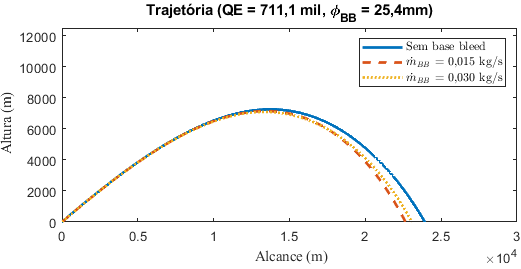
\includegraphics[width=0.7\textwidth]{foto1-qe711mil-1pol.png}
    \caption[QE = \qty{711}{\milliradian} \(\left(\phi_{BB} = \qty{25,4}{\millimetre}\right)\)]{QE = \qty{711}{\milliradian} \(\left(\phi_{BB} = \qty{25,4}{\millimetre}\right)\)}
    \label{fig:trajetoria-1pol-711mil}
\end{figure}

\begin{table}[ht]
\centering
\caption[Trajetória Balística com QE = \qty{711}{\milliradian} e v = \qty{878}{\metre\per\second} \(\left(\phi_{BB} = \qty{25,4}{\millimetre}\right)\)]{Trajetória Balística com QE = \qty{711}{\milliradian} e v = \qty{878}{\metre\per\second} \(\left(\phi_{BB} = \qty{25,4}{\millimetre}\right)\)}
\vspace{0.5cm}
\begin{tabular}{c|c|c|c|c}
Vazão Mássica & Alcance & Aumento & Apogeu & Aumento \\
\hline
\qty{0}{\kilogram\per\second} & \qty{23922,2}{\metre} & -- & \qty{7256,8}{\metre} & -- \\ 
\qty{0,015}{\kilogram\per\second} & \qty{22647,8}{\metre} & \qty{-5,3}{\percent} & \qty{7145,0}{\metre} & \qty{-1,5}{\percent} \\
\qty{0,030}{\kilogram\per\second} & \qty{23069,0}{\metre} & \qty{-3,6}{\percent} & \qty{7093,4}{\metre} & \qty{-2,3}{\percent}
\end{tabular}
\label{tab:tabela-711mil-bb-1pol}
\fonte{Autor.}
\end{table}

Acerca da \autoref{fig:trajetoria-1pol-800mil}, apesar de haver um aumento do alcance dos lançamentos sob efeito BB, os resultados também foram piores, quando comparados com o lançamento inerte. A \autoref{tab:tabela-800mil-bb-1pol} demonstra resultados percentuais muito próximos dos que foram apresentados na tabela anterior.

\begin{figure}[!ht]
	\centering
    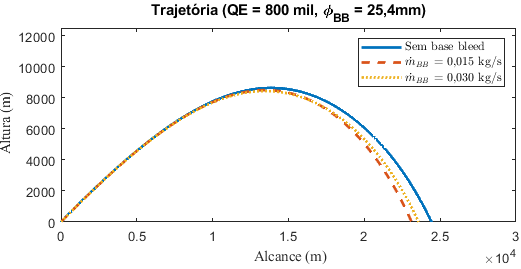
\includegraphics[width=0.7\textwidth]{foto2-qe800mil-1pol.png}
    \caption[QE = \qty{800}{\milliradian} \(\left(\phi_{BB} = \qty{25,4}{\millimetre}\right)\)]{QE = \qty{800}{\milliradian} \(\left(\phi_{BB} = \qty{25,4}{\millimetre}\right)\)}
    \label{fig:trajetoria-1pol-800mil}
\end{figure}

\begin{table}[ht]
\centering
\caption[Trajetória Balística com QE = \qty{800}{\milliradian} e v = \qty{878}{\metre\per\second} \(\left(\phi_{BB} = \qty{25,4}{\millimetre}\right)\)]{Trajetória Balística com QE = \qty{800}{\milliradian} e v = \qty{878}{\metre\per\second} \(\left(\phi_{BB} = \qty{25,4}{\millimetre}\right)\)}
\vspace{0.5cm}
\begin{tabular}{c|c|c|c|c}
Vazão Mássica & Alcance & Aumento & Apogeu & Aumento \\
\hline
\qty{0}{\kilogram\per\second} & \qty{24429,5}{\metre} & -- & \qty{8638,6}{\metre} & -- \\ 
\qty{0,015}{\kilogram\per\second} & \qty{23117,9}{\metre} & \qty{-5,4}{\percent} & \qty{8493,6}{\metre} & \qty{-1,7}{\percent} \\
\qty{0,030}{\kilogram\per\second} & \qty{23577,0}{\metre} & \qty{-3,5}{\percent} & \qty{8435,9}{\metre} & \qty{-2,3}{\percent}
\end{tabular}
\label{tab:tabela-800mil-bb-1pol}
\fonte{Autor.}
\end{table}

Ao verificar a \autoref{fig:trajetoria-2pol-711mil} percebe-se um aumento do alcance e do apogeu, atestado pela \autoref{tab:tabela-711mil-bb-2pol}. Há o aumento do alcance de quase \qty{6}{\percent} quando \(\Dot{m}_{BB} = \qty{0,060}{\kilogram\per\second}\).

\begin{figure}[!ht]
	\centering
    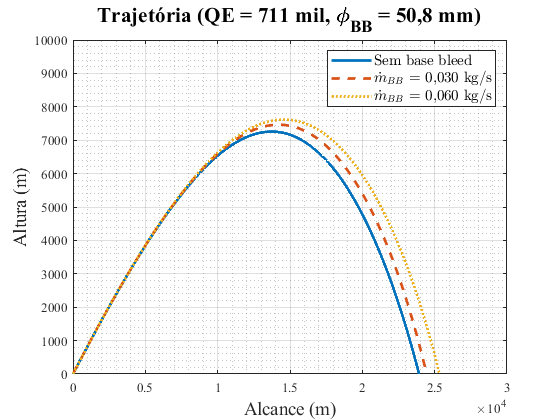
\includegraphics[width=0.7\textwidth]{foto3-qe711mil-2pol.png}
    \caption[QE = \qty{711}{\milliradian} \(\left(\phi_{BB} = \qty{50,8}{\millimetre}\right)\)]{QE = \qty{711}{\milliradian} \(\left(\phi_{BB} = \qty{50,8}{\millimetre}\right)\)}
    \label{fig:trajetoria-2pol-711mil}
\end{figure}

\begin{table}[!ht]
\centering
\caption[Trajetória Balística com QE = \qty{711}{\milliradian} e v = \qty{878}{\metre\per\second} \(\left(\phi_{BB} = \qty{50,8}{\millimetre}\right)\)]{Trajetória Balística com QE = \qty{711}{\milliradian} e v = \qty{878}{\metre\per\second} \(\left(\phi_{BB} = \qty{50,8}{\millimetre}\right)\)}
\vspace{0.5cm}
\begin{tabular}{c|c|c|c|c}
Vazão Mássica & Alcance & Aumento & Apogeu & Aumento \\
\hline
\qty{0}{\kilogram\per\second} & \qty{23922,2}{\metre} & -- & \qty{7256,8}{\metre} & -- \\
\qty{0,030}{\kilogram\per\second} & \qty{24439,8}{\metre} & \qty{2,2}{\percent} & \qty{7463,5}{\metre} & \qty{2,8}{\percent} \\
\qty{0,060}{\kilogram\per\second} & \qty{25334,3}{\metre} & \qty{5,9}{\percent} & \qty{7616,6}{\metre} & \qty{5,0}{\percent}
\end{tabular}
\label{tab:tabela-711mil-bb-2pol}
\fonte{Autor.}
\end{table}

Ao aumentar o ângulo de elevação para \qty{800}{\milliradian} houve um incremento percentual sobre o alcance e o apogeu também, como demonstrado na \autoref{fig:trajetoria-2pol-800mil}. Os resultados seguiram a mesma ordem de crescimento do deslocamento, quando se compara a \autoref{tab:tabela-711mil-bb-2pol} com a \autoref{tab:tabela-800mil-bb-2pol}. De qualquer forma, o diâmetro de saída do bocal tem forte influência na balística externa do projetil.

\begin{figure}[!ht]
	\centering
    \includegraphics[width=0.7\textwidth]{foto4-qe800mil-2pol.png}
    \caption[QE = \qty{800}{\milliradian} \(\left(\phi_{BB} = \qty{50,8}{\millimetre}\right)\)]{QE = \qty{800}{\milliradian} \(\left(\phi_{BB} = \qty{50,8}{\millimetre}\right)\)}
    \label{fig:trajetoria-2pol-800mil}
\end{figure}

\begin{table}[ht]
\centering
\caption[Trajetória Balística com QE = \qty{800}{\milliradian} e v = \qty{878}{\metre\per\second} \(\left(\phi_{BB} = \qty{50,8}{\millimetre}\right)\)]{Trajetória Balística com QE = \qty{800}{\milliradian} e v = \qty[per-mode = symbol]{878}{\metre\per\second} \(\left(\phi_{BB} = \qty{50,8}{\millimetre}\right)\)}
\vspace{0.5cm}
\begin{tabular}{c|c|c|c|c}
Vazão Mássica & Alcance & Aumento & Apogeu & Aumento \\
\hline
\qty{0}{\kilogram\per\second} & \qty{24429,5}{\metre} & -- & \qty{8638,6}{\metre} & -- \\ 
\qty{0,030}{\kilogram\per\second} & \qty{25030,7}{\metre} & \qty{2,5}{\percent} & \qty{8892,7}{\metre} & \qty{2,9}{\percent} \\
\qty{0,060}{\kilogram\per\second} & \qty{26008,5}{\metre} & \qty{6,5}{\percent} & \qty{9084,5}{\metre} & \qty{5,2}{\percent}
\end{tabular}
\label{tab:tabela-800mil-bb-2pol}
\fonte{Autor.}
\end{table}
\chapter{Comentários Finais}\label{cap:conclusoes}

O trabalho iniciou a partir da pesquisa bibliográfica sobre aerodinâmica de um projétil de artilharia. A partir deste ponto, duas regiões de domínio foram modeladas sob as mesmas condições de contorno. Definindo-se estas condições e modificando o regime de velocidade do escoamento, foram realizados testes com CFD a partir dos modelos RANS de turbulência Spalart-Allmaras \cite{Spalart1992} e SST $\kappa$-$\omega$ \cite{Menter1994TwoequationET,Menter2003,Menter2009}, considerando ou não o efeito \textit{Base Bleed}.

Como se trabalha com fenômenos de turbulência aplicados em escoamentos compressíveis, algumas simplificações foram implementadas nas simulações CFD: domínio bidimensional e axissimétrico, conforme as principais referências \cite{Mahmoud2009,Lucena2020}; regime estacionário, logo não se analisou a influência do tempo no escoamento; fluido como gás ideal para fechar o algoritmo \textit{density-based} com as equações de gases perfeitos para a pressão em função da densidade e temperatura e a viscosidade pela lei de Sutherland.

As primeiras soluções para os modelos SST $\kappa-\omega$ foram baseadas no projetil inerte (sem \textit{Base Bleed}) para análise de convergência, pautados em valores de referência \cite{Mahmoud2009} do coeficiente de arrasto aerodinâmico para um projetil de calibre 155mm. Duas malhas foram testadas sob o mesmo domínio computacional, a fim de analisar qualitativamente e quantitavimente os resultados de acordo com o número de elementos. Só então que foram verificadas as influências do diâmetro de injeção, \(\phi_{BB}\); da temperatura dos gases na saída do bocal, \(T_{BB}\), e da vazão do sistema \textit{Base Bleed}, \(\Dot{m}_{BB}\). Para o modelo Spalart-Allmaras (S-A), a verificação foi feita apenas com projetil ativo (com \textit{Base Bleed}) com diâmetro e vazão do sistema \textit{Base Bleed} fixados para verificar a diferença dos resultados entre as metodologias S-A e SST $\kappa-\omega$.

Utilizou-se o software Fluent \cite{fluent2021ansys} para aplicação dos modelos de turbulência e respectivas soluções. A abordagem de discretização do código é baseada no Método de Volumes Finitos \cite{McDonald1971,MacComarck&Paulay1972}. Todos os casos supracitados fizeram uso do esquema \textit{upwind} de segunda ordem para a discretização dos termos advectivos e difusivos. Para os gradientes das propriedades foi escolhido o método dos Mínimos Quadrados por ser um método mais barato computacionalmente \cite{fluent2021ansys}. Em razão do regime de voo do projetil, o algoritmo \textit{density-based} \cite{Weiss1995PreconditioningAT,Weiss1997IMPLICITSO,Weiss1999ImplicitSO} foi aplicado em razão da compressibilidade. Para resolução do sistemas algébricos gerados em cada simulação CFD o método \textit{multigrid} \cite{Hutchinson1986} foi selecionado. A conjunção dessas técnicas garantiu os resultados nos dois modelos RANS selecionados.

Os valores encontrados pelas simulações CFD possibilitaram a aplicação do modelo de trajetória ponto-massa modificado (MPMTM), padronização organizada pela OTAN \cite{stanag4355} e aplicada para projetis axissimétrica estabilizados pela rotação. Esse modelo tem o foco em reduzir custos computacionais quando comparado ao modelo de dinâmica de corpo rígido, inclusive para operações de combate, fazendo dele o mais indicado para elaboração de tabela de tiros de munições. O código desenvolvido em MATLAB\textregistered{} \cite{ThallyoENCIT2022,Thallyo2022} calculou as condições da munição 155mm disparadas em 2 ângulos de elevação diferentes; com e sem \textit{Base Bleed}; assim como a variação de parâmetros nos casos em que disparou o projetil ativo: o diâmetro de saída do bocal de injeção e a vazão mássica do propelente. 

\section{Conclusão}

Os resultados para as simulações de fluidodinâmica computacional mostraram uma tendência positiva no que se refere aos valores do coeficiente de arrasto, tendo em vista que a implementação da tecnologia \textit{Base Bleed} implica em mexer em parâmetros sensíveis, inclusive de design da munição. A abordagem deste estudo foi desenvolver estimativas iniciais, mesmo sem formulações químicas realísticas para simular a queima do propelente atuante na região a jusante do projetil. Contudo, os parâmetros avaliados como o diâmetro de saída do bocal de injeção, a temperatura e a vazão mostraram influência significativa nos resultados finais.

O modelo SST $\kappa-\omega$ conseguiu predizer os valores do $C_D$ para o projetil inerte com certa razoabilidade, assim como descrito nas referências \cite{Mahmoud2009,nicolas-perez_accuracy_2017}. Contudo, a interação entre a frente de chama do \textit{Base Bleed} e a esteira turbulenta presente na base do projetil dificulta as estimativas com maior acurácia usando modelos RANS \cite{nicolas-perez_accuracy_2017}. Em seu estudo, \citeauthor{Spalart1992} afirma que é difícil modelar um choque quando há um alto gradiente adverso de pressão, além de outros colaboradores da pesquisa deste artigo mencionarem que são produzidos resultados de baixa qualidade em escoamentos que há um degrau descendente (\textit{backward-facing step}) por causa das tensões produzidas. Este argumento também pode explicar a falta de precisão dos resultados na região após o \textit{boat-tail}.

Conforme visto nas referências, o regime transônico apresentou os valores mais elevados para o coeficiente de arrasto, enquanto o regime supersônico relatou uma queda mais gradual neste coeficiente com o aumento do número de Mach, com algumas singularidades ao mudar certas variáveis. O parâmetro mais relevante para mudar o arrasto de base foi o diâmetro de saída do bocal, apesar de tanto a vazão mássica e a temperatura mostrarem uma redução.

A implementação do software para o cálculo da trajetória com 4 graus de liberdade foi feita sem considerar os efeitos de ignição e com vazão constante do \textit{Base Bleed} durante toda a queima, o que não é um modelo realístico, tendo em vista que a taxa de queima de propelente tem grande influência da rotação e da pressão atmosférica. Como a geometria do projetil foi simplificada para se ter estimativas do $C_D$, a massa da câmara foi considerada apenas o conteúdo do propelente. Sabe-se que em projetis de artilharia a base contém cavidade, fora os componentes adicionados para fazer a propulsão sólida que adicionam massa e mudam a estrutura.

\section{Recomendações}

Espera-se em estudos futuros que novos fatores geométricos sejam considerados em projeto, como o design da câmara geradora de gás acoplada à munição; os efeitos de rotação do projetil; a contribuição do sistema de ignição para a tecnologia \textit{Base Bleed} e implementação de possíveis formulações para o propelente a ser inserido na câmara geradora de gás, já que assumir os gases em combustão como perfeitos é uma simplificação para garantir um ponto de partida do projeto. 

Em se tratando de simulações numéricas, recomenda-se implementar modelos de turbulência LES ou DNS para captar a mistura do jato do \textit{Base Bleed} com a esteira produzida no escoamento na base da munição, seguindo a linha das principais referências bibliográficas \cite{nicolas-perez_accuracy_2017,Lucena2020}. A simplificação da malha bidimensional e axissimétrica só foi possível pois não se estudou a influência do ângulo de ataque nos coeficientes aerodinâmicos. Portanto, um caminho natural para esta análise seria desenvolver uma malha tridimensional.

Com os avanços tecnológicos, espera-se que simulações com processamento em placa gráfica (GPU) possam ser utilizados para otimização dos resultados e permitindo análises mais refinadas, inclusive com malhas com um número maior de elementos e modelos de turbulência mais complexos do que os baseados em RANS.

Sobre o modelo de trajetória, um estudo de eficiência computacional para limpeza do código seria um passo concreto para otimização dos processos de predição de voo. O uso de uma linguagem de programação compilada além do MATLAB\textregistered{} também seria interessante para aumentar a velocidade de processamento, já que se trata de uma linguagem interpretada e por ser um produto comercial, tem restrições de uso para desenvolver um software que contemple os interesses de pesquisa e de transferência tecnológica para o Exército Brasileiro.

Finalmente, os estudos desenvolvidos neste projeto produziram conteúdos para publicação em congressos científicos, dentre os quais 1 publicação para a Revista Militar de Ciência e Tecnologia (RMCT) e 4 artigos para congressos de Engenharia realizados em 2022 (III CBCFD, XIX ENCIT, XI CONEM e XLIII CILAMCE). Acredita-se que esforços futuros em novas simulações numéricas permitam a esta linha de pesquisa um potencial de desenvolvimento tecnológico de interesse para o Exército Brasileiro. 

% ----------------------------------------------------------
% ELEMENTOS PÓS-TEXTUAIS1
% ----------------------------------------------------------
\postextual
% ----------------------------------------------------------

% ----------------------------------------------------------
% Referências bibliográficas
% ----------------------------------------------------------
\bibliography{refs}

% ----------------------------------------------------------
% Apêndices
% ----------------------------------------------------------

\begin{apendicesenv}
    \partapendices
    \chapter{Coeficientes Aerodinâmicos - Sem Base Bleed}\label{apend:apendice-sembb}

Neste apêndice, a \autoref{tab:apendice-coeficientes-sembasebleed} mostra os coeficientes aerodinâmicos calculados para o lançamento do projetil sem \textit{Base Bleed}.

\begin{table}[ht]
\centering
\caption[Coeficientes Aerodinâmicos (sem \textit{Base Bleed})]{Coeficientes Aerodinâmicos (sem \textit{Base Bleed})}
\vspace{0.5cm}
\begin{tabular}{c|c|c|c|c|c|c|c}
Mach & \(C_{D_0}\) & \(C_{D_{\alpha^2}}\) & \(C_{L_\alpha}\) & \(C_{mag-f}\) & \(C_{m_{\alpha}}\) & \(C_{spin}\) & \(C_{D_{BB}}\) \\\hline
0,01  & 0,1359  & 1,9800 & 1,6800 & -0,3550 & 3,2000 & -0,0270 & 0,0860 \\
0,4   & 0,1359  & 1,9800 & 1,6800 & -0,3550 & 3,2000 & -0,0270 & 0,0860 \\
0,6   & 0,1288  & 1,9900 & 1,6800 & -0,3550 & 3,3000 & -0,0270 & 0,0930 \\
0,7   & 0,06345 & 2,2200 & 1,6900 & -0,3600 & 3,3500 & -0,0260 & 0,0960 \\
0,75  & 0,1539  & 2,3100 & 1,6900 & -0,3600 & 3,4000 & -0,0250 & 0,0980 \\
0,8   & 0,10402 & 2,3900 & 1,7300 & -0,3700 & 3,5000 & -0,0250 & 0,1000 \\
0,85  & 0,20344 & 2,5300 & 1,7600 & -0,3800 & 3,6000 & -0,0240 & 0,1020 \\
0,875 & 0,2845  & 2,6400 & 1,8100 & -0,3850 & 3,7500 & -0,0240 & 0,1030 \\
0,9   & 0,19867 & 2,7400 & 1,8800 & -0,3950 & 3,9000 & -0,0240 & 0,1040 \\
0,925 & 0,2433  & 2,8600 & 1,9900 & -0,4450 & 4,2000 & -0,0240 & 0,1050 \\
0,95  & 0,26077 & 3,0000 & 2,0900 & -0,5050 & 4,2000 & -0,0230 & 0,1060 \\
0,975 & 0,2854  & 3,1800 & 2,1700 & -0,4500 & 4,0000 & -0,0230 & 0,1070 \\
1,0   & 0,3172  & 3,3900 & 2,2100 & -0,4150 & 3,7120 & -0,0248 & 0,0000 \\
1,025 & 0,3303  & 3,6100 & 2,2400 & -0,4650 & 3,5810 & -0,0248 & 0,0000 \\
1,05  & 0,3533  & 3,8400 & 2,2600 & -0,4450 & 3,4990 & -0,0246 & 0,0000 \\
1,1   & 0,3558  & 4,3500 & 2,2900 & -0,4150 & 3,4600 & -0,0242 & 0,0000 \\
1,2   & 0,3450  & 4,8210 & 2,3500 & -0,3750 & 3,4850 & -0,0238 & 0,0000 \\
1,35  & 0,3593  & 4,3100 & 2,4300 & -0,3400 & 3,4740 & -0,0230 & 0,0000 \\
1,5   & 0,3032  & 3,8100 & 2,5300 & -0,3250 & 3,2650 & -0,0222 & 0,0000 \\
1,75  & 0,2696  & 3,3400 & 2,6400 & -0,3150 & 3,0660 & -0,0212 & 0,0000 \\
2,0   & 0,2589  & 2,8100 & 2,7400 & -0,2950 & 3,0070 & -0,0206 & 0,0000 \\
2,25  & 0,2366  & 2,5100 & 2,8000 & -0,2900 & 2,9210 & -0,0198 & 0,0000 \\
2,5   & 0,2227  & 2,2300 & 2,8100 & -0,2900 & 2,8770 & -0,0192 & 0,0000 \\
3,0   & 0,1962  & 1,7800 & 2,7700 & -0,2900 & 2,8280 & -0,0180 & 0,0000
\end{tabular}
\label{tab:apendice-coeficientes-sembasebleed}
\end{table}
    \chapter{Coeficientes Aerodinâmicos - Temperatura de Saída 300K}\label{apend:apendice-combb300K}

Neste apêndice, a \autoref{tab:apendice-coeficientes-combasebleed-300K} mostra os coeficientes aerodinâmicos calculados são para o lançamento do projetil com \textit{Base Bleed} em que a temperatura de saída dos gases foi fixada em 300K.

\begin{table}[ht]
\centering
\caption[Coeficientes Aerodinâmicos (com Base Bleed - \(T_{BB}\) = 300K)]{Coeficientes Aerodinâmicos (com Base Bleed - \(T_{BB}\) = 300K)}
\vspace{0.5cm}
\begin{tabular}{c|c|c|c|c|c|c|c}
    Mach & \(C_{D_0}\) & \(C_{D_{\alpha^2}}\) & \(C_{L_\alpha}\) & \(C_{mag-f}\) & \(C_{m_{\alpha}}\) & \(C_{spin}\) & \(C_{D_{BB}}\) \\\hline
0,01  & 0,1705 & 1,9800 & 1,6800 & -0,3550 & 3,2000 & -0,0270 & 0,0860 \\
0,4   & 0,1705 & 1,9800 & 1,6800 & -0,3550 & 3,2000 & -0,0270 & 0,0860 \\
0,6   & 0,1342 & 1,9900 & 1,6800 & -0,3550 & 3,3000 & -0,0270 & 0,0930 \\
0,7   & 0,1265 & 2,2200 & 1,6900 & -0,3600 & 3,3500 & -0,0260 & 0,0960 \\
0,75  & 0,1499 & 2,3100 & 1,6900 & -0,3600 & 3,4000 & -0,0250 & 0,0980 \\
0,8   & 0,1210 & 2,3900 & 1,7300 & -0,3700 & 3,5000 & -0,0250 & 0,1000 \\
0,85  & 0,1319 & 2,5300 & 1,7600 & -0,3800 & 3,6000 & -0,0240 & 0,1020 \\
0,875 & 0,1286 & 2,6400 & 1,8100 & -0,3850 & 3,7500 & -0,0240 & 0,1030 \\
0,9   & 0,1578 & 2,7400 & 1,8800 & -0,3950 & 3,9000 & -0,0240 & 0,1040 \\
0,925 & 0,2129 & 2,8600 & 1,9900 & -0,4450 & 4,2000 & -0,0240 & 0,1050 \\
0,95  & 0,2100 & 3,0000 & 2,0900 & -0,5050 & 4,2000 & -0,0230 & 0,1060 \\
0,975 & 0,3152 & 3,1800 & 2,1700 & -0,4500 & 4,0000 & -0,0230 & 0,1070 \\
1,0   & 0,3641 & 3,3900 & 2,2100 & -0,4150 & 3,7120 & -0,0248 & 0,0000 \\
1,025 & 0,3724 & 3,6100 & 2,2400 & -0,4650 & 3,5810 & -0,0248 & 0,0000 \\
1,05  & 0,3795 & 3,8400 & 2,2600 & -0,4450 & 3,4990 & -0,0246 & 0,0000 \\
1,1   & 0,3805 & 4,3500 & 2,2900 & -0,4150 & 3,4600 & -0,0242 & 0,0000 \\
1,2   & 0,3675 & 4,8210 & 2,3500 & -0,3750 & 3,4850 & -0,0238 & 0,0000 \\
1,35  & 0,3454 & 4,3100 & 2,4300 & -0,3400 & 3,4740 & -0,0230 & 0,0000 \\
1,5   & 0,3254 & 3,8100 & 2,5300 & -0,3250 & 3,2650 & -0,0222 & 0,0000 \\
1,75  & 0,2950 & 3,3400 & 2,6400 & -0,3150 & 3,0660 & -0,0212 & 0,0000 \\
2,0   & 0,2711 & 2,8100 & 2,7400 & -0,2950 & 3,0070 & -0,0206 & 0,0000 \\
2,25  & 0,2499 & 2,5100 & 2,8000 & -0,2900 & 2,9210 & -0,0198 & 0,0000 \\
2,5   & 0,2314 & 2,2300 & 2,8100 & -0,2900 & 2,8770 & -0,0192 & 0,0000 \\
3,0   & 0,2023 & 1,7800 & 2,7700 & -0,2900 & 2,8280 & -0,0180 & 0,0000
\end{tabular}
\label{tab:apendice-coeficientes-combasebleed-300K}
\end{table}
    \chapter{Coeficientes Aerodinâmicos - Temperatura de saída 1500K}

Neste apêndice, a \autoref{tab:apendice-coeficientes-combasebleed-1500K} mostra os coeficientes aerodinâmicos calculados para o lançamento do projetil com \textit{Base Bleed} em que a temperatura de saída dos gases foi fixada em 1500K.

\begin{table}[ht]
\centering
\caption[Coeficientes Aerodinâmicos (com Base Bleed - \(T_{BB}\) = 1500K)]{Coeficientes Aerodinâmicos (com Base Bleed - \(T_{BB}\) = 1500K)}
\vspace{0.5cm}
\begin{tabular}{c|c|c|c|c|c|c|c}
    Mach & \(C_{D_0}\) & \(C_{D_{\alpha^2}}\) & \(C_{L_\alpha}\) & \(C_{mag-f}\) & \(C_{m_{\alpha}}\) & \(C_{spin}\) & \(C_{D_{BB}}\) \\\hline
0,01  & 0,1705  & 1,9800 & 1,6800 & -0,3550 & 3,2000 & -0,0270 & 0,0860 \\
0,4   & 0,1705  & 1,9800 & 1,6800 & -0,3550 & 3,2000 & -0,0270 & 0,0860 \\
0,6   & 0,1342  & 1,9900 & 1,6800 & -0,3550 & 3,3000 & -0,0270 & 0,0930 \\
0,7   & 0,12857 & 2,2200 & 1,6900 & -0,3600 & 3,3500 & -0,0260 & 0,0960 \\
0,75  & 0,1499  & 2,3100 & 1,6900 & -0,3600 & 3,4000 & -0,0250 & 0,0980 \\
0,8   & 0,12349 & 2,3900 & 1,7300 & -0,3700 & 3,5000 & -0,0250 & 0,1000 \\
0,85  & 0,13390 & 2,5300 & 1,7600 & -0,3800 & 3,6000 & -0,0240 & 0,1020 \\
0,875 & 0,1452  & 2,6400 & 1,8100 & -0,3850 & 3,7500 & -0,0240 & 0,1030 \\
0,9   & 0,15865 & 2,7400 & 1,8800 & -0,3950 & 3,9000 & -0,0240 & 0,1040 \\
0,925 & 0,2129  & 2,8600 & 1,9900 & -0,4450 & 4,2000 & -0,0240 & 0,1050 \\
0,95  & 0,21207 & 3,0000 & 2,0900 & -0,5050 & 4,2000 & -0,0230 & 0,1060 \\
0,975 & 0,3152  & 3,1800 & 2,1700 & -0,4500 & 4,0000 & -0,0230 & 0,1070 \\
1,0   & 0,3660  & 3,3900 & 2,2100 & -0,4150 & 3,7120 & -0,0248 & 0,0000 \\
1,025 & 0,3744  & 3,6100 & 2,2400 & -0,4650 & 3,5810 & -0,0248 & 0,0000 \\
1,05  & 0,3812  & 3,8400 & 2,2600 & -0,4450 & 3,4990 & -0,0246 & 0,0000 \\
1,1   & 0,3814  & 4,3500 & 2,2900 & -0,4150 & 3,4600 & -0,0242 & 0,0000 \\
1,2   & 0,3673  & 4,8210 & 2,3500 & -0,3750 & 3,4850 & -0,0238 & 0,0000 \\
1,35  & 0,3438  & 4,3100 & 2,4300 & -0,3400 & 3,4740 & -0,0230 & 0,0000 \\
1,5   & 0,3233  & 3,8100 & 2,5300 & -0,3250 & 3,2650 & -0,0222 & 0,0000 \\
1,75  & 0,2943  & 3,3400 & 2,6400 & -0,3150 & 3,0660 & -0,0212 & 0,0000 \\
2,0   & 0,2698  & 2,8100 & 2,7400 & -0,2950 & 3,0070 & -0,0206 & 0,0000 \\
2,25  & 0,2493  & 2,5100 & 2,8000 & -0,2900 & 2,9210 & -0,0198 & 0,0000 \\
2,5   & 0,2286  & 2,2300 & 2,8100 & -0,2900 & 2,8770 & -0,0192 & 0,0000 \\
3,0   & 0,1963  & 1,7800 & 2,7700 & -0,2900 & 2,8280 & -0,0180 & 0,0000
\end{tabular}
\label{tab:apendice-coeficientes-combasebleed-1500K}
\end{table}
    \chapter{Coeficientes Aerodinâmicos - Diâmetro 1 polegada e Vazão 15 g/s}

Neste apêndice, a \autoref{tab:apendice-coeficientes-bb-1pol-0015} mostra os coeficientes aerodinâmicos calculados são para o lançamento do projetil com \textit{Base Bleed} em que a temperatura de saída dos gases foi fixada em 2306,15K, o diâmetro da saída do bocal foi de 25,4 mm (1 polegada) e vazão mássica de 0,015 kg/s.

\begin{table}[ht]
\centering
\caption[Coeficientes Aerodinâmicos (com Base Bleed - \(\phi_{BB}\) = 25,4mm, \(\Dot{m}_{BB}\) = 0,015 kg/s e \(T_{BB}\) = 2306,15K)]{Coeficientes Aerodinâmicos  (com Base Bleed - \(\phi_{BB}\) = 25,4mm, \(\Dot{m}_{BB}\) = 0,015 kg/s e \(T_{BB}\) = 2306,15K)}
\vspace{0.5cm}
\begin{tabular}{c|c|c|c|c|c|c|c}
    Mach & \(C_{D_0}\) & \(C_{D_{\alpha^2}}\) & \(C_{L_\alpha}\) & \(C_{mag-f}\) & \(C_{m_{\alpha}}\) & \(C_{spin}\) & \(C_{D_{BB}}\) \\\hline
0,01  & 0,1561  & 1,9800 & 1,6800 & -0,3550 & 3,2000 & -0,0270 & 0,0860 \\
0,4   & 0,1561  & 1,9800 & 1,6800 & -0,3550 & 3,2000 & -0,0270 & 0,0860 \\
0,6   & 0,1654  & 1,9900 & 1,6800 & -0,3550 & 3,3000 & -0,0270 & 0,0930 \\
0,7   & 0,04748 & 2,2200 & 1,6900 & -0,3600 & 3,3500 & -0,0260 & 0,0960 \\
0,75  & 0,1982  & 2,3100 & 1,6900 & -0,3600 & 3,4000 & -0,0250 & 0,0980 \\
0,8   & 0,15409 & 2,3900 & 1,7300 & -0,3700 & 3,5000 & -0,0250 & 0,1000 \\
0,85  & 0,24103 & 2,5300 & 1,7600 & -0,3800 & 3,6000 & -0,0240 & 0,1020 \\
0,875 & 0,3356  & 2,6400 & 1,8100 & -0,3850 & 3,7500 & -0,0240 & 0,1030 \\
0,9   & 0,17424 & 2,7400 & 1,8800 & -0,3950 & 3,9000 & -0,0240 & 0,1040 \\
0,925 & 0,2601  & 2,8600 & 1,9900 & -0,4450 & 4,2000 & -0,0240 & 0,1050 \\
0,95  & 0,27058 & 3,0000 & 2,0900 & -0,5050 & 4,2000 & -0,0230 & 0,1060 \\
0,975 & 0,3020  & 3,1800 & 2,1700 & -0,4500 & 4,0000 & -0,0230 & 0,1070 \\
1,0   & 0,3593  & 3,3900 & 2,2100 & -0,4150 & 3,7120 & -0,0248 & 0,0000 \\
1,025 & 0,3701  & 3,6100 & 2,2400 & -0,4650 & 3,5810 & -0,0248 & 0,0000 \\
1,05  & 0,3822  & 3,8400 & 2,2600 & -0,4450 & 3,4990 & -0,0246 & 0,0000 \\
1,1   & 0,4013  & 4,3500 & 2,2900 & -0,4150 & 3,4600 & -0,0242 & 0,0000 \\
1,2   & 0,3878  & 4,8210 & 2,3500 & -0,3750 & 3,4850 & -0,0238 & 0,0000 \\
1,35  & 0,3857  & 4,3100 & 2,4300 & -0,3400 & 3,4740 & -0,0230 & 0,0000 \\
1,5   & 0,3445  & 3,8100 & 2,5300 & -0,3250 & 3,2650 & -0,0222 & 0,0000 \\
1,75  & 0,3019  & 3,3400 & 2,6400 & -0,3150 & 3,0660 & -0,0212 & 0,0000 \\
2,0   & 0,2829  & 2,8100 & 2,7400 & -0,2950 & 3,0070 & -0,0206 & 0,0000 \\
2,25  & 0,2644  & 2,5100 & 2,8000 & -0,2900 & 2,9210 & -0,0198 & 0,0000 \\
2,5   & 0,2417  & 2,2300 & 2,8100 & -0,2900 & 2,8770 & -0,0192 & 0,0000 \\
3,0   & 0,2163  & 1,7800 & 2,7700 & -0,2900 & 2,8280 & -0,0180 & 0,0000
\end{tabular}
\label{tab:apendice-coeficientes-bb-1pol-0015}
\end{table}
    \chapter{Coeficientes Aerodinâmicos - Diâmetro 1 Polegada e Vazão 30 g/s}

Neste apêndice, a \autoref{tab:apendice-coeficientes-bb-1pol-0030} mostra os coeficientes aerodinâmicos calculados são para o lançamento do projetil com \textit{Base Bleed} em que a temperatura de saída dos gases foi fixada em 2306,15K, o diâmetro da saída do bocal foi de 25,4mm (1 polegada) e vazão mássica de 0,030 kg/s.

\begin{table}[ht]
\centering
\caption[Coeficientes Aerodinâmicos (com Base Bleed - \(\phi_{BB}\) = 25,4mm, \(\Dot{m}_{BB}\) = 0,030 kg/s e \(T_{BB}\) = 2306,15K)]{Coeficientes Aerodinâmicos  (com Base Bleed - \(\phi_{BB}\) = 25,4mm, \(\Dot{m}_{BB}\) = 0,030 kg/s e \(T_{BB}\) = 2306,15K)}
\vspace{0.5cm}
\begin{tabular}{c|c|c|c|c|c|c|c}
    Mach & \(C_{D_0}\) & \(C_{D_{\alpha^2}}\) & \(C_{L_\alpha}\) & \(C_{mag-f}\) & \(C_{m_{\alpha}}\) & \(C_{spin}\) & \(C_{D_{BB}}\) \\\hline
0,01  & 0,1750  & 1,9800 & 1,6800 & -0,3550 & 3,2000 & -0,0270 & 0,0860 \\
0,4   & 0,1750  & 1,9800 & 1,6800 & -0,3550 & 3,2000 & -0,0270 & 0,0860 \\
0,6   & 0,1691  & 1,9900 & 1,6800 & -0,3550 & 3,3000 & -0,0270 & 0,0930 \\
0,7   & 0,21505 & 2,2200 & 1,6900 & -0,3600 & 3,3500 & -0,0260 & 0,0960 \\
0,75  & 0,1701  & 2,3100 & 1,6900 & -0,3600 & 3,4000 & -0,0250 & 0,0980 \\
0,8   & 0,13850 & 2,3900 & 1,7300 & -0,3700 & 3,5000 & -0,0250 & 0,1000 \\
0,85  & 0,21317 & 2,5300 & 1,7600 & -0,3800 & 3,6000 & -0,0240 & 0,1020 \\
0,875 & 0,1734  & 2,6400 & 1,8100 & -0,3850 & 3,7500 & -0,0240 & 0,1030 \\
0,9   & 0,18623 & 2,7400 & 1,8800 & -0,3950 & 3,9000 & -0,0240 & 0,1040 \\
0,925 & 0,2382  & 2,8600 & 1,9900 & -0,4450 & 4,2000 & -0,0240 & 0,1050 \\
0,95  & 0,24622 & 3,0000 & 2,0900 & -0,5050 & 4,2000 & -0,0230 & 0,1060 \\
0,975 & 0,3371  & 3,1800 & 2,1700 & -0,4500 & 4,0000 & -0,0230 & 0,1070 \\
1,0   & 0,3675  & 3,3900 & 2,2100 & -0,4150 & 3,7120 & -0,0248 & 0,0000 \\
1,025 & 0,3985  & 3,6100 & 2,2400 & -0,4650 & 3,5810 & -0,0248 & 0,0000 \\
1,05  & 0,4032  & 3,8400 & 2,2600 & -0,4450 & 3,4990 & -0,0246 & 0,0000 \\
1,1   & 0,4038  & 4,3500 & 2,2900 & -0,4150 & 3,4600 & -0,0242 & 0,0000 \\
1,2   & 0,3897  & 4,8210 & 2,3500 & -0,3750 & 3,4850 & -0,0238 & 0,0000 \\
1,35  & 0,3658  & 4,3100 & 2,4300 & -0,3400 & 3,4740 & -0,0230 & 0,0000 \\
1,5   & 0,3441  & 3,8100 & 2,5300 & -0,3250 & 3,2650 & -0,0222 & 0,0000 \\
1,75  & 0,3131  & 3,3400 & 2,6400 & -0,3150 & 3,0660 & -0,0212 & 0,0000 \\
2,0   & 0,2871  & 2,8100 & 2,7400 & -0,2950 & 3,0070 & -0,0206 & 0,0000 \\
2,25  & 0,2652  & 2,5100 & 2,8000 & -0,2900 & 2,9210 & -0,0198 & 0,0000 \\
2,5   & 0,2464  & 2,2300 & 2,8100 & -0,2900 & 2,8770 & -0,0192 & 0,0000 \\
3,0   & 0,2160  & 1,7800 & 2,7700 & -0,2900 & 2,8280 & -0,0180 & 0,0000
\end{tabular}
\label{tab:apendice-coeficientes-bb-1pol-0030}
\end{table}
    \chapter{Coeficientes Aerodinâmicos - Diâmetro 2 polegadas e Vazão 30 g/s}

Neste apêndice, a \autoref{tab:apendice-coeficientes-bb-2pol-0030} mostra os coeficientes aerodinâmicos calculados são para o lançamento do projetil com \textit{Base Bleed} em que a temperatura de saída dos gases foi fixada em 2306,15K, o diâmetro da saída do bocal foi de 50,8mm (2 polegadas) e vazão mássica de 0,030 kg/s.

\begin{table}[ht]
\centering
\caption[Coeficientes Aerodinâmicos (com Base Bleed - $\phi_{bb}$ = 50,8mm, $\Dot{m}_{bb}$ = 0,030 kg/s e $T_{bb}$ = 2306,15K)]{Coeficientes Aerodinâmicos  (com Base Bleed - $\phi_{bb}$ = 50,8mm, $\Dot{m}_{bb}$ = 0,030 kg/s e $T_{bb}$ = 2306,15K)}
\vspace{0.5cm}
\begin{tabular}{c|c|c|c|c|c|c|c}
    Mach & \(C_{X_0}\) & \(C_{X_{\alpha^2}}\) & \(C_{Z_\alpha}\) & \(C_{mag-f}\) & \(C_{m_{\alpha}}\) & \(C_{spin}\) & \(C_{X_b}\) \\\hline
0,01  & 0,1294  & 1,9800 & 1,6800 & -0,3550 & 3,2000 & -0,0270 & 0,0860 \\
0,4   & 0,1294  & 1,9800 & 1,6800 & -0,3550 & 3,2000 & -0,0270 & 0,0860 \\
0,6   & 0,0720  & 1,9900 & 1,6800 & -0,3550 & 3,3000 & -0,0270 & 0,0930 \\
0,7   & 0,14091 & 2,2200 & 1,6900 & -0,3600 & 3,3500 & -0,0260 & 0,0960 \\
0,75  & 0,1620  & 2,3100 & 1,6900 & -0,3600 & 3,4000 & -0,0250 & 0,0980 \\
0,8   & 0,12645 & 2,3900 & 1,7300 & -0,3700 & 3,5000 & -0,0250 & 0,1000 \\
0,85  & 0,15056 & 2,5300 & 1,7600 & -0,3800 & 3,6000 & -0,0240 & 0,1020 \\
0,875 & 0,1100  & 2,6400 & 1,8100 & -0,3850 & 3,7500 & -0,0240 & 0,1030 \\
0,9   & 0,15525 & 2,7400 & 1,8800 & -0,3950 & 3,9000 & -0,0240 & 0,1040 \\
0,925 & 0,2069  & 2,8600 & 1,9900 & -0,4450 & 4,2000 & -0,0240 & 0,1050 \\
0,95  & 0,22370 & 3,0000 & 2,0900 & -0,5050 & 4,2000 & -0,0230 & 0,1060 \\
0,975 & 0,3108  & 3,1800 & 2,1700 & -0,4500 & 4,0000 & -0,0230 & 0,1070 \\
1,0   & 0,3278  & 3,3900 & 2,2100 & -0,4150 & 3,7120 & -0,0248 & 0,0000 \\
1,025 & 0,3390  & 3,6100 & 2,2400 & -0,4650 & 3,5810 & -0,0248 & 0,0000 \\
1,05  & 0,3535  & 3,8400 & 2,2600 & -0,4450 & 3,4990 & -0,0246 & 0,0000 \\
1,1   & 0,3556  & 4,3500 & 2,2900 & -0,4150 & 3,4600 & -0,0242 & 0,0000 \\
1,2   & 0,3543  & 4,8210 & 2,3500 & -0,3750 & 3,4850 & -0,0238 & 0,0000 \\
1,35  & 0,3348  & 4,3100 & 2,4300 & -0,3400 & 3,4740 & -0,0230 & 0,0000 \\
1,5   & 0,3127  & 3,8100 & 2,5300 & -0,3250 & 3,2650 & -0,0222 & 0,0000 \\
1,75  & 0,2815  & 3,3400 & 2,6400 & -0,3150 & 3,0660 & -0,0212 & 0,0000 \\
2,0   & 0,2633  & 2,8100 & 2,7400 & -0,2950 & 3,0070 & -0,0206 & 0,0000 \\
2,25  & 0,2438  & 2,5100 & 2,8000 & -0,2900 & 2,9210 & -0,0198 & 0,0000 \\
2,5   & 0,2278  & 2,2300 & 2,8100 & -0,2900 & 2,8770 & -0,0192 & 0,0000 \\
3,0   & 0,2000  & 1,7800 & 2,7700 & -0,2900 & 2,8280 & -0,0180 & 0,0000
\end{tabular}
\label{tab:apendice-coeficientes-bb-2pol-0030}
\end{table}
    \chapter{Coeficientes Aerodinâmicos - Diâmetro 2 polegadas e Vazão 60 g/s}\label{apend:apendice-combb-2pol-006}

Neste apêndice, a \autoref{tab:apendice-coeficientes-bb-2pol-0060} mostra os coeficientes aerodinâmicos calculados são para o lançamento do projetil com \textit{Base Bleed} em que a temperatura de saída dos gases foi fixada em 2306,15K, o diâmetro da saída do bocal foi de 50,8mm (2 polegadas) e vazão mássica de 0,060 kg/s.

\begin{table}[ht]
\centering
\caption[Coeficientes Aerodinâmicos (com Base Bleed - $\phi_{bb}$ = 50,8mm, $\Dot{m}_{bb}$ = 0,060 kg/s e $T_{bb}$ = 2306,15K)]{Coeficientes Aerodinâmicos  (com Base Bleed - $\phi_{bb}$ = 50,8mm, $\Dot{m}_{bb}$ = 0,060 kg/s e $T_{bb}$ = 2306,15K)}
\vspace{0.5cm}
\begin{tabular}{c|c|c|c|c|c|c|c}
Mach & $C_{X_0}$ & $C_{X_{\alpha^2}}$ & $C_{Z_\alpha}$ & $C_{mag-f}$ & $C_{m_{\alpha}}$ & $C_{spin}$ & $C_{X_b}$ \\\hline
0,01  & 0,1359  & 1,9800 & 1,6800 & -0,3550 & 3,2000 & -0,0270 & 0,0860 \\
0,4   & 0,1359  & 1,9800 & 1,6800 & -0,3550 & 3,2000 & -0,0270 & 0,0860 \\
0,6   & 0,1288  & 1,9900 & 1,6800 & -0,3550 & 3,3000 & -0,0270 & 0,0930 \\
0,7   & 0,06345 & 2,2200 & 1,6900 & -0,3600 & 3,3500 & -0,0260 & 0,0960 \\
0,75  & 0,1539  & 2,3100 & 1,6900 & -0,3600 & 3,4000 & -0,0250 & 0,0980 \\
0,8   & 0,10402 & 2,3900 & 1,7300 & -0,3700 & 3,5000 & -0,0250 & 0,1000 \\
0,85  & 0,20344 & 2,5300 & 1,7600 & -0,3800 & 3,6000 & -0,0240 & 0,1020 \\
0,875 & 0,2845  & 2,6400 & 1,8100 & -0,3850 & 3,7500 & -0,0240 & 0,1030 \\
0,9   & 0,19867 & 2,7400 & 1,8800 & -0,3950 & 3,9000 & -0,0240 & 0,1040 \\
0,925 & 0,2433  & 2,8600 & 1,9900 & -0,4450 & 4,2000 & -0,0240 & 0,1050 \\
0,95  & 0,26077 & 3,0000 & 2,0900 & -0,5050 & 4,2000 & -0,0230 & 0,1060 \\
0,975 & 0,2854  & 3,1800 & 2,1700 & -0,4500 & 4,0000 & -0,0230 & 0,1070 \\
1,0   & 0,3172  & 3,3900 & 2,2100 & -0,4150 & 3,7120 & -0,0248 & 0,0000 \\
1,025 & 0,3303  & 3,6100 & 2,2400 & -0,4650 & 3,5810 & -0,0248 & 0,0000 \\
1,05  & 0,3533  & 3,8400 & 2,2600 & -0,4450 & 3,4990 & -0,0246 & 0,0000 \\
1,1   & 0,3558  & 4,3500 & 2,2900 & -0,4150 & 3,4600 & -0,0242 & 0,0000 \\
1,2   & 0,3450  & 4,8210 & 2,3500 & -0,3750 & 3,4850 & -0,0238 & 0,0000 \\
1,35  & 0,3593  & 4,3100 & 2,4300 & -0,3400 & 3,4740 & -0,0230 & 0,0000 \\
1,5   & 0,3032  & 3,8100 & 2,5300 & -0,3250 & 3,2650 & -0,0222 & 0,0000 \\
1,75  & 0,2696  & 3,3400 & 2,6400 & -0,3150 & 3,0660 & -0,0212 & 0,0000 \\
2,0   & 0,2589  & 2,8100 & 2,7400 & -0,2950 & 3,0070 & -0,0206 & 0,0000 \\
2,25  & 0,2366  & 2,5100 & 2,8000 & -0,2900 & 2,9210 & -0,0198 & 0,0000 \\
2,5   & 0,2227  & 2,2300 & 2,8100 & -0,2900 & 2,8770 & -0,0192 & 0,0000 \\
3,0   & 0,1962  & 1,7800 & 2,7700 & -0,2900 & 2,8280 & -0,0180 & 0,0000
\end{tabular}
\label{tab:apendice-coeficientes-bb-2pol-0060}
\end{table}
\end{apendicesenv}
% ---

%---------------------------------------------------------------------
% INDICE REMISSIVO
%---------------------------------------------------------------------
\phantompart
\printindex
%---------------------------------------------------------------------

\end{document}